%% ============================================================================
%% MMRDR Diabetic-Retinopathy Internship Report
%% Built on the supplied IEEE template (ieeecolor.cls + generic.sty).
%% Figures live in ./figures/.  Compile: pdflatex report.tex  (x2 for refs)
%% ============================================================================
\documentclass[journal,twoside,web]{ieeecolor}
\usepackage{generic}
\usepackage{cite}
\usepackage{amsmath,amssymb,amsfonts}
\usepackage{algorithmic}
\usepackage{graphicx}
\usepackage{textcomp}
\usepackage{hyperref}
\hypersetup{hidelinks=true}
\graphicspath{{figures/}}

\markboth{MMRDR Diabetic Retinopathy --- Internship Report}
{Baghla: Multi-Task Deep-Learning Baselines for Diabetic Retinopathy on the MMRDR Dataset}

\begin{document}

% ---------------------------------------------------------------------------
\title{Multi-Task Deep-Learning Baselines for Diabetic Retinopathy Grading and Lesion Detection on the Multimodal MMRDR Dataset}

\author{Krrish Baghla
\thanks{This work was carried out by Krrish Baghla as a research intern in the
Department of Computer Science and Engineering, Indian Institute of Technology
(BHU), Varanasi, India (e-mail: krrishbaghla108@gmail.com).}
\thanks{The internship was supervised by Dr.~Sanjay Kumar Singh, Professor,
Department of Computer Science and Engineering, Indian Institute of Technology
(BHU), Varanasi, India (e-mail: sks.cse@iitbhu.ac.in).}}

\maketitle

\begin{abstract}
Diabetic retinopathy (DR) is a leading cause of preventable blindness, and its
automated screening from retinal images is a well-motivated clinical
application of deep learning. This report documents a set of multi-task
deep-learning baselines developed on the Multimodal Retinal Diabetic-Retinopathy
(MMRDR) dataset, which spans color fundus photography (CFP), ultra-widefield
(UWF), and optical coherence tomography modalities. Each baseline jointly
performs five-class DR severity grading and seven-way multi-label lesion
detection from a single shared representation. We present eleven experiments. The
first three establish modality baselines: a multi-scale dual-branch convolutional
network on CFP, a fine-tuned RETFound retinal foundation model on CFP, and a
feature-pyramid network with spatial attention on UWF, attaining grade accuracies
of 82.91\%, 80.94\%, and 74.48\% respectively. The RETFound experiment reproduces
the published MMRDR baseline on the dataset's official test split, matching three
of its four reported metrics within 95\% confidence intervals; an earlier attempt
had reported only 66.50\%, which an audit traced to a silent weight-loading failure
in which just 4 of 294 tensors transferred. The remaining
seven form a focused study on the ultra-widefield modality aimed at the rare,
sight-threatening lesions of proliferative DR (neovascularization, vitreous
haemorrhage, retinal detachment), attacked from six angles: a clinically-weighted
lesion loss that lifts retinal-detachment recall to 0.79; an asymmetric
false-negative-penalised focal loss reaching a quadratic Cohen's $\kappa$ of 0.92
and lesion AUC of 0.95; a supervised contrastive auxiliary; learned homoscedastic
uncertainty weighting, which reaches the study's best rare-lesion detection (lesion
F1 up to 0.778, AUROC up to 0.961); a recall-driven curriculum resampler that
drives retinal-detachment recall to 1.0 on a stratified split; a controlled,
capacity-matched head ablation showing on a held-out test split that a dedicated
rare-lesion head does not help; and a conditional-diffusion generator for synthetic
minority augmentation whose downstream test returns a clean negative verdict (adding
$64$px synthetic images does not beat a real-only baseline on rare-class recall, with
a high synthetic-vs-real FID explaining why). A concluding experiment tests
cross-dataset generalization: the two CFP models and a UWF control are evaluated
zero-shot and few-shot on two unseen external datasets (APTOS~2019 and IDRiD), where
the RETFound foundation model transfers best, grading unseen fundus images zero-shot
at a quadratic $\kappa$ of $0.86$. Models are trained with
transfer learning, focal-family objectives for class imbalance, mixed-precision
optimisation, and early stopping, and are interpreted using gradient-weighted class
activation mapping (Grad-CAM), which confirms that predictions are driven by
clinically plausible retinal regions. The report details the objective,
methodology, architecture, training procedure, and results of each experiment, and
reports honest limitations including a saturated uncertainty clamp, single-seed
passes, and non-comparable splits.
\end{abstract}

\begin{IEEEkeywords}
Class imbalance, contrastive learning, convolutional neural networks, curriculum
learning, deep learning, diabetic retinopathy, diffusion models, explainable
artificial intelligence, fundus imaging, generative augmentation, medical image
analysis, multi-task learning, transfer learning, ultra-widefield imaging,
uncertainty weighting.
\end{IEEEkeywords}

% ===========================================================================
\section{Introduction}
\label{sec:introduction}
\IEEEPARstart{D}{iabetic} retinopathy (DR) is a microvascular complication of
diabetes and one of the leading causes of preventable vision loss worldwide.
Clinical management depends on grading disease severity---typically on a
five-point ordinal scale from no DR (grade~0) to proliferative DR
(grade~4)---and on identifying the retinal lesions that characterise each stage.
Because expert screening does not scale to the diabetic population, automated
analysis of retinal images with deep neural networks has become an active area
of research.

This internship uses the Multimodal Retinal Diabetic-Retinopathy (MMRDR)
dataset~\cite{mmrdr}, which provides labelled images across three complementary
modalities: color fundus photography (CFP), ultra-widefield (UWF) imaging, and
optical coherence tomography. Every image is annotated with a DR severity grade
and a seven-element multi-label lesion vector in the fixed order
$[\text{MA},\text{HE},\text{IH},\text{VB/IRMA},\text{NV},\text{VH},\text{RD}]$.
The two tasks are clinically coupled: the presence of specific lesions
determines the grade, which motivates a \emph{multi-task} formulation in which a
single network predicts both the grade and the lesion vector from a shared
representation.

Ten self-contained experiments are examined in this report, all sharing the same
multi-task objective. The first three establish modality baselines. Experiment~I
develops a custom multi-scale dual-branch convolutional network on CFP.
Experiment~II fine-tunes the RETFound retinal foundation model~\cite{retfound} on
the same CFP data and reproduces the published MMRDR baseline on the dataset's
official train/test partition. Experiment~III adapts a feature-pyramid architecture
with spatial attention to the higher-resolution UWF modality.

The remaining five experiments pursue a single research question on the UWF
modality: how to make a multi-task model sensitive to the rare, sight-threatening
lesions that define proliferative DR---neovascularization (NV), vitreous
haemorrhage (VH), and retinal detachment (RD)---which occupy indices $4$--$6$ of
the lesion vector and are severely under-represented. They attack it from four
complementary angles. Experiment~IV re-weights the lesion loss by combined
statistical rarity and clinical risk. Experiment~V replaces the objective with an
asymmetric loss that penalises false negatives on those lesions far more than false
positives~\cite{asl}. Experiment~VI adds a supervised contrastive
auxiliary~\cite{supcon} that shapes the feature space around rare-lesion images.
Experiment~VII replaces the fixed task weights with learned homoscedastic-uncertainty
weights~\cite{uncertainty}. Experiment~VIII leaves the network untouched and adapts
the training \emph{sampler} with a recall-driven curriculum built on an
effective-number rarity prior~\cite{effnum}. Finally, two experiments probe the
architecture and the data supply: Experiment~IX is a controlled, capacity-matched
ablation of the lesion head on a held-out test split, and Experiment~X trains a
conditional-diffusion~\cite{ddpm} generator that \emph{synthesises} rare-lesion
images rather than oversampling them and tests them downstream (a clean negative
verdict: they do not beat a real-only baseline). The ten trained experiments rely on transfer learning from
ImageNet- or RETFound-pretrained weights, use focal-family objectives~\cite{focalloss}
to counter class imbalance, and are interpreted with Grad-CAM~\cite{gradcam} to
verify that predictions attend to clinically relevant regions. This document reports
the objective, methodology, architecture, training procedure, and measured results
of each experiment in turn.

% ===========================================================================
\section{Materials and Dataset}
\label{sec:materials}
All experiments draw on the MMRDR dataset~\cite{mmrdr}. Each modality is stored
in its own subdirectory with an image folder and a metadata CSV whose columns
are \texttt{type}, \texttt{image}, \texttt{grade}, \texttt{lesion}, and
\texttt{lr}. The \texttt{grade} column encodes the five-class DR severity label,
and the \texttt{lesion} column encodes the seven-element multi-label lesion
vector as a bracketed string. Experiments~I and~II use the CFP subset
(\texttt{FP.csv}); Experiments~III--X use the UWF subset (\texttt{UWF.csv}).

Two splitting protocols appear in this report and should not be conflated. Most
experiments follow the repository convention of an 80/20 split with
\texttt{random\_state}~$=42$, in which the held-out 20\% partition serves as the
per-epoch validation set and is also the set on which results are reported.
Experiments~II and~IX instead reserve a genuine held-out test partition that is
evaluated only once: Experiment~IX uses a stratified 70/15/15 three-way split, and
Experiment~II uses the dataset's \emph{official} partition, which is encoded in the
image file names (\texttt{tr} for the $8{,}893$ training images, \texttt{ts} for the
$2{,}225$ test images) and is the partition on which the published MMRDR baselines
were measured. Accuracies obtained under these two protocols are not directly
comparable. Modality-specific image counts, preprocessing, and splits are reported
within each experiment.

% ===========================================================================
\section{Experiment I: Multi-Scale Dual-Branch CNN on CFP}
\label{sec:exp1}

\subsection{Objective}
The objective of Experiment~I is to train a single convolutional network that
simultaneously performs (i)~five-class DR severity grading and (ii)~seven-way
multi-label lesion detection on color fundus photographs, from a shared feature
representation.

\subsection{Motivation}
Color fundus photography is the most widely available DR screening modality, so a
strong CFP baseline is the natural starting point. DR-defining lesions
(e.g.\ microaneurysms) are small relative to the field of view, yet grading also
requires global context such as the distribution of haemorrhages and the optic
disc. A single-scale classifier tends to trade one against the other. This
motivates a \emph{multi-scale} design that preserves fine, early-layer detail
alongside deep semantic context, and a multi-task head that lets the grade and
lesion objectives regularise a common backbone.

\subsection{Methodology}
The approach is a multi-task convolutional network, \texttt{MultiScaleDRNet},
built on a ResNet-50 backbone~\cite{resnet} initialised from ImageNet weights.
Fine-grained features from an early residual stage and semantic features from the
final stage are channel-aligned and fused before branching into a grade head and
a lesion head. Class imbalance in the ordinal grade is addressed with a focal
loss~\cite{focalloss}, and model behaviour is examined with Grad-CAM~\cite{gradcam}.

\subsection{Experimental Setup}
Experiments were implemented in PyTorch and run on a single CUDA GPU with
automatic mixed precision (AMP) enabled. Gradient accumulation was used to reach
a larger effective batch size, and \texttt{cudnn.benchmark} was enabled. Model
selection used validation grade accuracy with early stopping.

\subsection{Dataset}
The CFP subset (\texttt{MMRDR-CFP/FP.csv}) comprises $11{,}118$ images. An 80/20
split with \texttt{random\_state}~$=42$ yields approximately $8{,}894$ training
and $2{,}224$ validation images. The split is random (not stratified by grade),
and the validation partition also serves as the reported evaluation set. Grade
imbalance is handled by the focal-loss objective rather than by resampling or
class weighting.

\subsection{Preprocessing}
Each fundus image is passed through a circular field-of-view mask
(\texttt{tightness}~$=0.96$): the image is cropped to its non-black bounding box
and all pixels outside an inscribed circle are zeroed, removing camera border
artifacts. Images are resized to $512\times512$ to preserve small lesions and
normalised with ImageNet statistics ($\mu=[0.485,0.456,0.406]$,
$\sigma=[0.229,0.224,0.225]$). Training augmentation comprises random horizontal
and vertical flips, random rotation ($\pm15^{\circ}$), and mild colour jitter
(brightness and contrast $0.1$); the validation transform applies only the mask,
resize, and normalisation.

\subsection{Architecture}
\texttt{MultiScaleDRNet} uses the ResNet-50 stem and residual stages
\texttt{layer1}--\texttt{layer4}. Two branches capture complementary scales.
The \emph{early} branch takes the \texttt{layer1} feature map (256 channels),
applies a $1\times1$ convolution to $512$ channels with batch normalisation, and
adaptively pools it to a $16\times16$ grid, retaining fine lesion-scale detail.
The \emph{deep} branch takes the \texttt{layer4} feature map ($2048$ channels)
and projects it to $512$ channels with batch normalisation, capturing global
semantics. The two $512$-channel maps are fused by element-wise addition
followed by a ReLU nonlinearity, globally average-pooled to a $512$-dimensional
vector, and passed to two linear heads: \texttt{head\_a\_lesion}
($512\!\rightarrow\!7$, multi-label) and \texttt{head\_b\_grade}
($512\!\rightarrow\!5$). The forward pass returns the grade and lesion logits
jointly.

\subsection{Training Procedure}
Training was scheduled for up to $50$ epochs with early stopping (patience $8$)
monitoring validation grade accuracy; the best checkpoint was saved to
\texttt{best\_multiscale\_resnet.pth} whenever grade accuracy improved. The run
stopped early at epoch $22$, with the best model obtained at \textbf{epoch~14}.
Training used AMP with a gradient scaler and gradient-norm clipping at $1.0$.

\subsection{Hyperparameters}
The training configuration is summarised in Table~\ref{tab:exp1_hyper}.

\begin{table}[!t]
\caption{Experiment~I --- Training Configuration}
\label{tab:exp1_hyper}
\centering
\setlength{\tabcolsep}{5pt}
\begin{tabular}{|l|l|}
\hline
\textbf{Setting} & \textbf{Value} \\
\hline
Backbone & ResNet-50 (ImageNet-pretrained) \\
Input resolution & $512\times512$ \\
Optimiser & AdamW \\
Learning rate & $3\times10^{-4}$ (constant) \\
Weight decay & $1\times10^{-4}$ \\
Batch size & $12$ (grad.\ accum.\ $2$ $\rightarrow$ eff.\ $24$) \\
Gradient clipping & max-norm $1.0$ \\
Mixed precision & Enabled (AMP) \\
Grade loss & Focal loss ($\gamma=2$) \\
Lesion loss & BCE-with-logits ($\times1.5$) \\
Epochs (planned / run) & $50$ / $22$ (early stop, patience $8$) \\
Best epoch & $14$ \\
\hline
\end{tabular}
\end{table}

The combined objective is
$\mathcal{L}=\mathcal{L}_{\text{grade}}^{\text{focal}}+1.5\,
\mathcal{L}_{\text{lesion}}^{\text{BCE}}$, weighting the lesion term slightly
higher than the grade term.

\subsection{Evaluation Metrics}
Two metrics are recorded each epoch: top-1 grade accuracy over the five-class
severity label, and element-wise multi-label lesion accuracy at a $0.5$ decision
threshold over the seven lesion outputs.

\subsection{Results}
The best validation grade accuracy is \textbf{0.8291} (82.91\%), reached at
epoch~14, while lesion accuracy remains high and stable throughout, peaking at
$0.9515$ at epoch~20 ($0.9494$ at the best-grade epoch). Table~\ref{tab:exp1_res}
summarises the headline figures, and Fig.~\ref{fig:exp1_curves} shows the
training loss and validation-accuracy trajectories. Fig.~\ref{fig:exp1_pred}
shows qualitative predictions on validation images, and Fig.~\ref{fig:exp1_cam}
shows Grad-CAM attributions for the grade and lesion heads.

\begin{table}[!t]
\caption{Experiment~I --- Best Validation Results}
\label{tab:exp1_res}
\centering
\setlength{\tabcolsep}{5pt}
\begin{tabular}{|l|c|c|}
\hline
\textbf{Metric} & \textbf{Best value} & \textbf{Epoch} \\
\hline
Grade accuracy & $0.8291$ & $14$ \\
Lesion accuracy (element-wise) & $0.9515$ & $20$ \\
Lesion accuracy at best-grade epoch & $0.9494$ & $14$ \\
\hline
\end{tabular}
\end{table}

\begin{figure}[!t]
\centerline{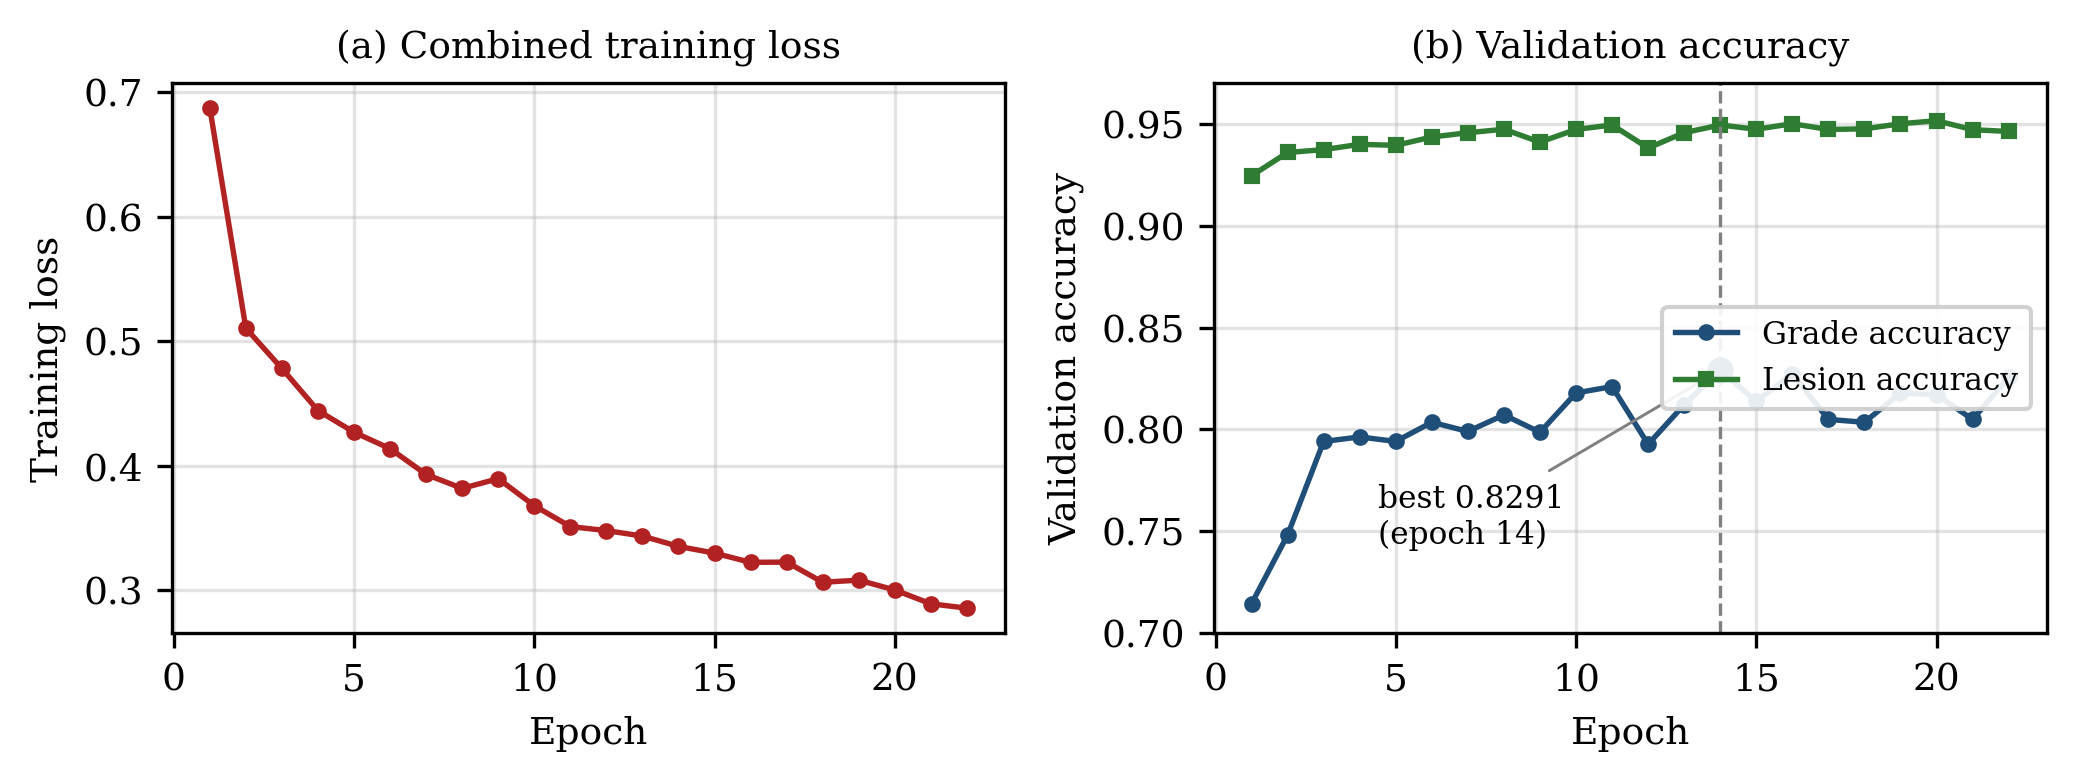
\includegraphics[width=\columnwidth]{exp1-training-curves.png}}
\caption{Experiment~I training dynamics. (a)~The combined grade-plus-lesion
training loss decreases monotonically from $0.687$ to $0.286$ over $22$ epochs.
(b)~Validation grade accuracy rises quickly and plateaus near $0.80$--$0.83$,
with the best value ($0.8291$) at epoch~14 (dashed line); element-wise lesion
accuracy stays high throughout.}
\label{fig:exp1_curves}
\end{figure}

\begin{figure*}[!t]
\centerline{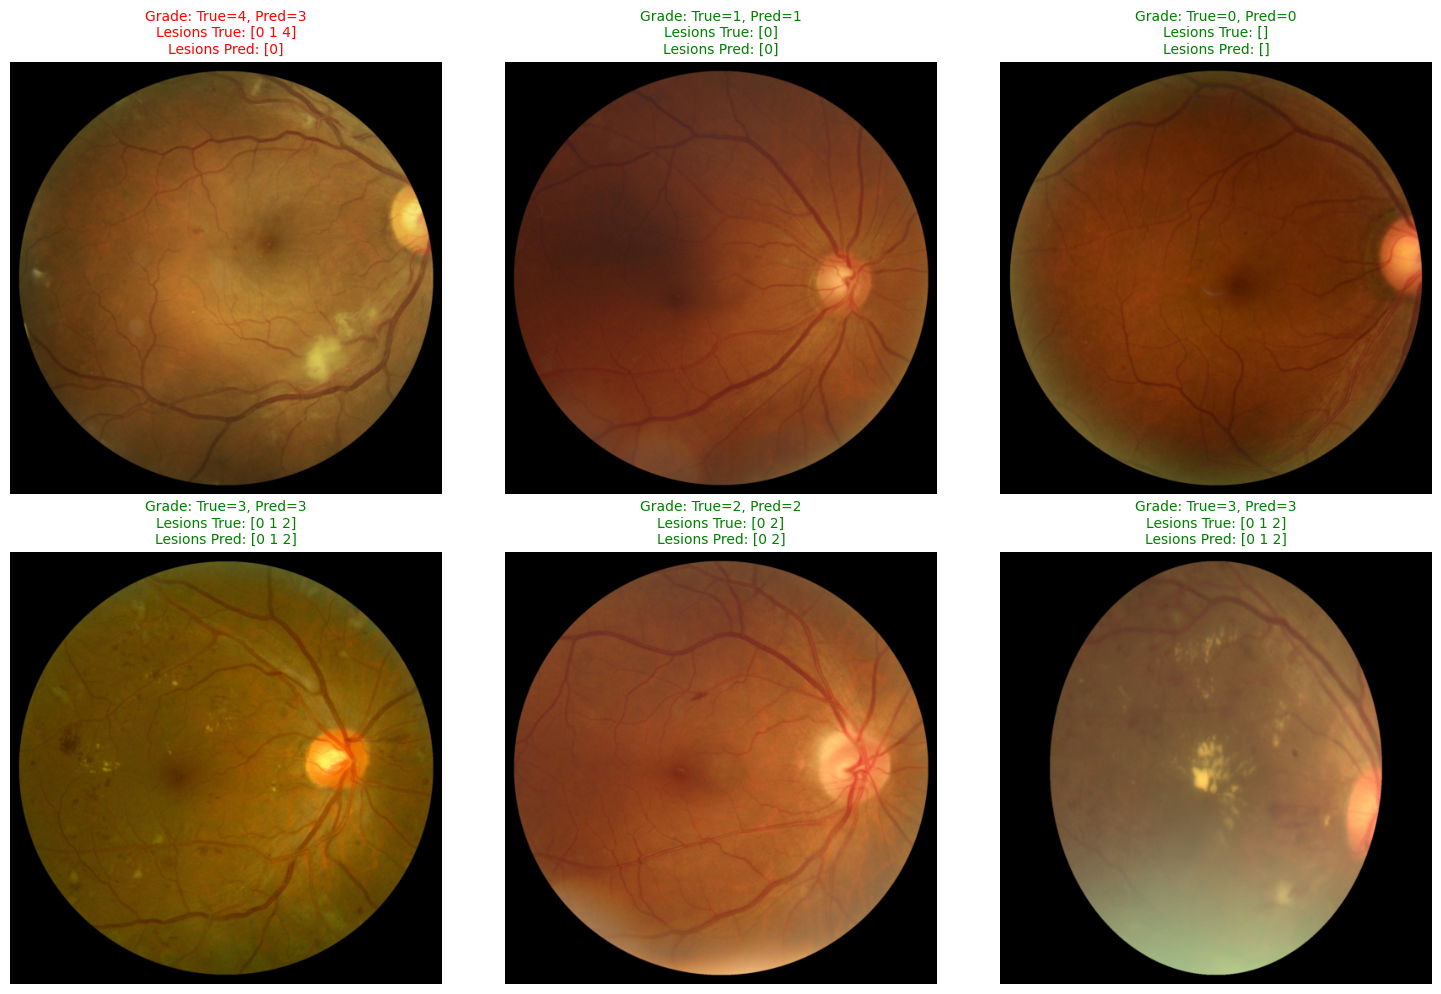
\includegraphics[width=0.9\textwidth]{exp1-predictions.png}}
\caption{Qualitative predictions of \texttt{MultiScaleDRNet} on CFP validation
images. Each panel reports the true and predicted DR grade and the true and
predicted lesion indices (green when the grade prediction is correct, red when
incorrect). The model recovers the grade and dominant lesions on most cases and
tends to confuse adjacent severity grades on the hardest examples.}
\label{fig:exp1_pred}
\end{figure*}

\begin{figure*}[!t]
\centerline{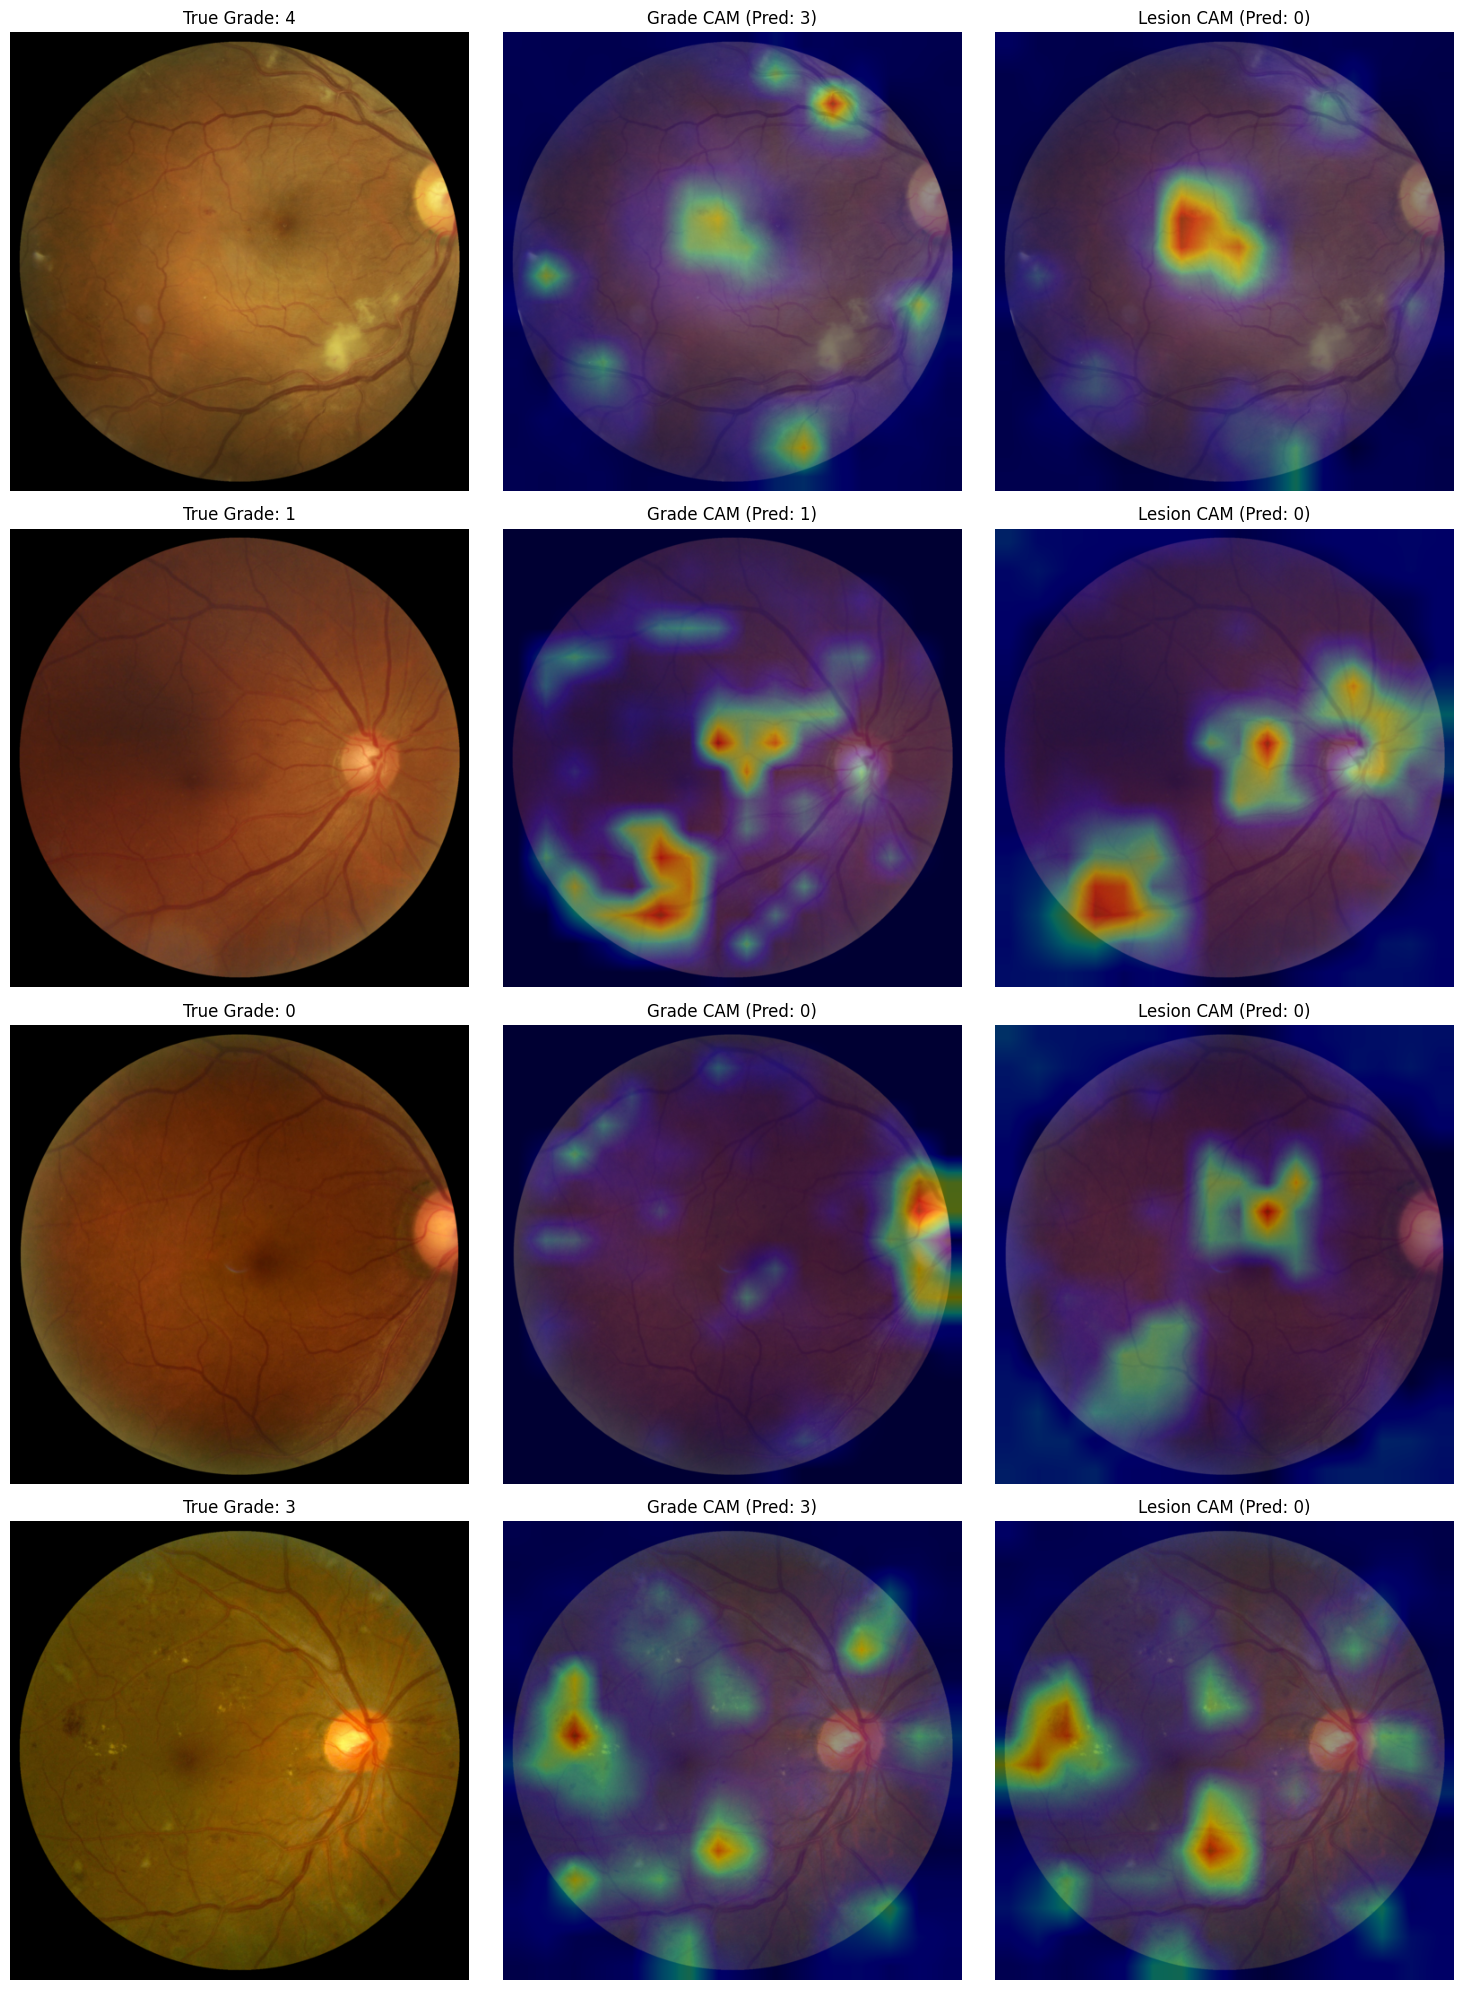
\includegraphics[width=0.92\textwidth]{exp1-gradcam.png}}
\caption{Grad-CAM~\cite{gradcam} attributions for \texttt{MultiScaleDRNet}.
For each fundus image (left) the grade-head activation map (centre) and
lesion-head activation map (right) highlight the regions driving the prediction.
Attention concentrates on the optic disc, vascular arcades, and bright/dark
lesion foci---clinically plausible evidence rather than background---supporting
the model's decisions.}
\label{fig:exp1_cam}
\end{figure*}

\subsection{Analysis}
The loss curve in Fig.~\ref{fig:exp1_curves}(a) falls smoothly and without
instability, indicating a well-behaved optimisation under AMP and gradient
clipping. Validation grade accuracy improves rapidly during the first ten epochs
and then oscillates within a narrow band around $0.80$--$0.83$, so early stopping
at the epoch-14 optimum is well justified. Lesion accuracy is consistently high
($\ge0.94$ after a few epochs); because it is measured element-wise over a sparse
multi-label target, it should be read as a stability indicator rather than a
measure of lesion-detection difficulty. The Grad-CAM maps in
Fig.~\ref{fig:exp1_cam} show that the grade and lesion heads localise onto the
optic disc, vasculature, and lesion foci, confirming that the multi-scale fusion
attends to clinically meaningful structures.

\subsection{Discussion}
The dual-branch design meets its intent: fusing early, high-resolution features
with deep semantic features yields a grade accuracy ($0.8291$) consistent with
the reproduced CFP baseline target and does so while jointly predicting lesions
from the same representation. The focal loss keeps the ordinal grade objective
stable despite class imbalance, and the qualitative and Grad-CAM figures indicate
that the network's competence is grounded in retinal anatomy rather than
spurious cues. As a multi-task CFP baseline it is the strongest of the three
experiments reported here.

\subsection{Limitations}
Several factors bound the strength of the reported figure. The train/test split
is random rather than stratified by grade, so rare high-severity grades may be
unevenly represented, and the validation partition doubles as the evaluation set.
No global random seed is fixed (only the split seed), so exact run-to-run
reproducibility is limited. The steadily falling training loss against a
plateauing validation accuracy indicates mild overfitting after the mid-training
optimum. Finally, the experiment covers the CFP modality only.

\subsection{Conclusion}
Experiment~I establishes a multi-task, multi-scale CFP baseline that reaches
$82.91\%$ validation grade accuracy while jointly detecting lesions and producing
interpretable Grad-CAM evidence. It serves as the convolutional reference point for
the report, noting that its figure is a validation accuracy on a random split and
so is not directly comparable to the held-out test accuracy of Experiment~II.

% ===========================================================================
\section{Experiment II: Reproducing the RETFound Foundation-Model Baseline on CFP}
\label{sec:exp2}

\subsection{Objective}
Experiment~II reproduces the RETFound~\cite{retfound} colour-fundus baseline published
with the MMRDR dataset~\cite{mmrdr}. The dataset paper reports, for RETFound fine-tuned
on MMRDR-CFP, a grade accuracy of $0.822$, grade F1 of $0.714$, lesion accuracy of
$0.951$, and lesion F1 of $0.682$. The objective here is to match those four numbers
under the paper's own protocol---full fine-tuning at $512\times512$ on the dataset's
official train/test partition---and, in doing so, to correct an earlier attempt that
reported only $66.50\%$ grade accuracy.

\subsection{Motivation}
A foundation model pretrained on 1.6 million retinal images should transfer strongly to
DR grading. An initial attempt in this project appeared to contradict that, reaching only
$66.50\%$. Rather than accept the result, the loading path was audited. The audit found
that the reported number was not a RETFound result at all, which makes this experiment as
much a lesson in verification as in transfer learning: a silent failure in a
weight-loading routine is indistinguishable from a genuine negative result unless it is
explicitly tested for.

\subsection{Diagnosis of the Earlier Attempt}
Three defects were identified, the first of which invalidates the earlier number entirely.

\emph{(i) The pretrained weights never loaded.} RETFound distributes an MAE ViT-Large
checkpoint whose parameters follow the \texttt{timm} naming convention
(\texttt{blocks.$i$.*}, \texttt{cls\_token}, \texttt{pos\_embed}). The earlier notebook
remapped those names onto \texttt{torchvision}'s \texttt{vit\_l\_16} by string
substitution, which is not a valid correspondence: \texttt{torchvision} requires
\texttt{encoder.layers.encoder\_layer\_$i$.*} together with different submodule names
(\texttt{ln\_1}, \texttt{self\_attention.in\_proj\_weight}, \texttt{mlp.0}), and expects
\texttt{class\_token} and \texttt{encoder.pos\_embedding}. Because the load was performed
with \texttt{strict=False}, the $290$ non-matching tensors were discarded without warning
and an unconditional success message was printed. Only $4$ of $294$ tensors---the
patch-embedding convolution and the final LayerNorm---were actually transferred. The
network was therefore a \emph{randomly initialised} ViT-Large trained on $8{,}894$
images, a regime in which large vision transformers are known to perform poorly.

\emph{(ii) The layer-freezing code had no effect.} The routine derived a block index with
\texttt{int(name.split(".")[3])}; for a parameter such as
\texttt{encoder.layers.encoder\_layer\_0.ln\_1.weight} that position is the string
\texttt{"ln\_1"}, so the conversion raised \texttt{ValueError} and the loop skipped every
parameter. No layer was ever frozen, despite the stated strategy of training only the
final six blocks.

\emph{(iii) Protocol weaknesses.} There was no learning-rate schedule or warmup, no fixed
random seed, the split was random rather than the dataset's official one, the validation
set doubled as the test set, and only accuracy was recorded.

\subsection{Methodology}
The corrected experiment removes the remapping step entirely by constructing the backbone
with \texttt{timm}, whose parameter names match the RETFound checkpoint natively. The
position embedding is the only tensor whose shape differs between the $224$ and $512$
input grids, and it is explicitly interpolated. Every stage of the load is then asserted
rather than assumed, and the trained model is evaluated once on the untouched official
test split.

\subsection{Experimental Setup}
Implemented in PyTorch on two Tesla T4 GPUs (\texttt{DataParallel}). Turing GPUs
(\texttt{sm\_75}) provide no native \texttt{bfloat16} arithmetic, so mixed precision uses
\texttt{float16} with gradient scaling; gradient checkpointing is enabled because a
ViT-Large at $512\times512$ processes $1{,}025$ tokens per image. A global seed is fixed
and the split is recorded as a hash so the partition is verifiable across runs.

\subsection{Dataset}
The MMRDR-CFP subset contains $11{,}118$ images whose file names encode the dataset's
\emph{official} partition: $8{,}893$ training images prefixed \texttt{tr} and $2{,}225$
test images prefixed \texttt{ts}. This experiment uses that partition, so its numbers are
directly comparable to the published baseline. A stratified $15\%$ of the training
portion---balanced jointly on DR grade and on the presence of a rare lesion---is held out
for validation, giving $7{,}559$ training, $1{,}334$ validation, and $2{,}225$ test
images (split signature \texttt{8ba3ee31bb06}). The three partitions were asserted
disjoint. Grade~0 accounts for $59.11\%$ of the training data, and the seven-element
lesion matrix is $13.97\%$ positive, so a trivial all-negative lesion predictor already
scores $0.8632$ element-wise---a floor that any lesion accuracy must be read against.

\subsection{Preprocessing}
Images are resized to $512\times512$ with bicubic interpolation and normalised with
ImageNet statistics. Training augmentation comprises random resized cropping
(scale $0.5$--$1.0$), random horizontal and vertical flips, and colour jitter;
validation and test apply only the resize and normalisation. No field-of-view mask is
applied in the headline configuration, since the published protocol specifies a plain
resize.

\subsection{Architecture}
The backbone is \texttt{timm}'s \texttt{vit\_large\_patch16\_224} instantiated at
\texttt{img\_size}~$=512$ with \texttt{global\_pool}~$=$~\texttt{avg} and
\texttt{drop\_path\_rate}~$=0.2$. Average pooling over patch tokens followed by an
\texttt{fc\_norm} layer reproduces RETFound's own \texttt{models\_vit.py} formulation. The
checkpoint's encoder LayerNorm is reused to initialise \texttt{fc\_norm} rather than
discarding it, a minor and deliberate deviation from the reference implementation. Two
linear heads read the pooled $1024$-d feature: a five-way grade head and a seven-way
lesion head. The forward pass returns only these small logit tensors, which keeps the
\texttt{DataParallel} output gather negligible.

\subsection{Verification of the Weight Load}
Three independent checks replace the earlier silent failure, each of which raises rather
than reports.

\emph{Key matching.} All $288$ transformer-block tensors matched
($288/288$, $100\%$), with no missing and no unexpected keys, and the position embedding
was interpolated from $(1,197,1024)$ to $(1,1025,1024)$. The routine aborts below a $95\%$
block-match threshold. The checkpoint is identified in the results record by a SHA-256
prefix (\texttt{61c20fc6d13c30d4}) so the exact file is provable.

\emph{Weight statistics.} All $294$ tensors differ from a freshly initialised model, and
the standard deviation of the attention projection varies with depth
($0.0216$ at block~0 rising to $0.0328$ at block~8), whereas a randomly initialised
transformer is flat at $\approx0.020$ everywhere. This test uses no parameter names and
so cannot be satisfied by a naming coincidence.

\emph{Functional probe.} With the backbone frozen and only a linear head trained, grade
accuracy reaches $0.6475$ against a majority-class baseline of $0.5907$. A randomly
initialised ViT-Large cannot exceed the majority baseline; the earlier configuration
would have failed this test.

\subsection{Training Procedure}
All $304{,}161{,}804$ parameters are trainable and none are frozen, matching the
published full fine-tuning setting; this is asserted at run time. Rather than freezing
layers outright, layer-wise learning-rate decay ($0.65$) scales the learning rate by
depth, from $2.63\times10^{-9}$ at the patch embedding to $1.25\times10^{-4}$ at the
heads---a graded alternative to a binary freeze that preserves generic early features
while adapting the upper blocks. Training ran the full $30$ epochs in approximately
$9.5$ hours; early stopping (patience $8$) was never triggered.

\subsection{Hyperparameters}
Table~\ref{tab:exp2_hyper} lists the configuration.

\begin{table}[!t]
\caption{Experiment~II --- Training Configuration}
\label{tab:exp2_hyper}
\centering
\setlength{\tabcolsep}{5pt}
\begin{tabular}{|l|l|}
\hline
\textbf{Setting} & \textbf{Value} \\
\hline
Backbone & \texttt{timm} ViT-L/16, \texttt{global\_pool=avg} \\
Input resolution & $512\times512$ (pos.\ embed.\ $197\!\rightarrow\!1025$) \\
Parameters & $304{,}161{,}804$ (all trainable, $0$ frozen) \\
Optimiser & AdamW, $\beta=(0.9,0.999)$ \\
Learning rate & $1.25\times10^{-4}$ ($\mathrm{blr}\,10^{-3}\!\times\!32/256$) \\
Layer-wise LR decay & $0.65$ \\
Schedule & $3$ warmup epochs, then cosine to $10^{-6}$ \\
Weight decay & $0.05$ (none on 1-D params / tokens) \\
Batch size & $8$/GPU $\times2$ GPUs $\times$ accum.\ $2$ (eff.\ $32$) \\
Mixed precision & \texttt{float16} + \texttt{GradScaler} (\texttt{sm\_75}) \\
Gradient checkpointing & Enabled (peak $13.5$\,GB) \\
Drop path / label smoothing & $0.2$ / $0.1$ \\
Gradient clipping & max-norm $1.0$ \\
Epochs & $30$ (completed; patience $8$ unused) \\
\hline
\end{tabular}
\end{table}

\subsection{Evaluation Metrics}
The four published quantities are reported: grade accuracy and macro-F1, and lesion
element-wise (Hamming) accuracy and macro-F1. Lesion accuracy is element-wise rather than
exact-match because an all-negative predictor scores $0.8632$ under the former, placing
the published $0.951$ about nine points above the floor, whereas exact-match agreement
would be far lower. Quadratic-weighted Cohen's~$\kappa$, macro-AUROC, macro-PR-AUC,
per-lesion statistics, and $1{,}000$-sample bootstrap confidence intervals are reported
alongside.

\subsection{Results}
Table~\ref{tab:exp2_res} compares the held-out test results with the published baseline.
Three of the four metrics contain the published value inside their $95\%$ confidence
interval and are therefore statistical matches: grade accuracy $0.8094$ (CI
$[0.792,0.825]$ versus $0.822$), grade macro-F1 $0.6920$ (CI $[0.665,0.718]$ versus
$0.714$), and lesion accuracy $0.9476$ (CI $[0.943,0.951]$ versus $0.951$). Lesion
macro-F1 at the fixed $0.5$ threshold is $0.6051$, below the published $0.682$; with
per-lesion thresholds fitted on validation it rises to $0.6743$.

Supporting metrics are strong: quadratic $\kappa$ $=0.8838$, macro-AUROC $=0.9706$,
macro-PR-AUC $=0.7412$, and MCC $=0.6735$. Relative to the earlier defective run, grade
accuracy improves from $0.6650$ to $0.8094$, an increase of $14.4$ points attributable to
the corrected weight load rather than to longer training.
Fig.~\ref{fig:exp2_curves} shows the training trajectories and
Fig.~\ref{fig:exp2_breakdown} the test-set breakdown.

\begin{table}[!t]
\caption{Experiment~II --- Reproduction of the Published RETFound CFP Baseline}
\label{tab:exp2_res}
\centering
\setlength{\tabcolsep}{3pt}
\begin{tabular}{|l|c|c|c|c|}
\hline
\textbf{Metric} & \textbf{Paper} & \textbf{Ours @0.5} & \textbf{95\% CI} & \textbf{Tuned} \\
\hline
Grade acc.\ (AccG) & $0.822$ & $0.8094$ & $[0.792,0.825]$ & $0.8094$ \\
Grade F1 (F1G) & $0.714$ & $0.6920$ & $[0.665,0.718]$ & $0.6920$ \\
Lesion acc.\ (AccL) & $0.951$ & $0.9476$ & $[0.943,0.951]$ & $0.9415$ \\
Lesion F1 (F1L) & $0.682$ & $0.6051$ & $[0.570,0.636]$ & $\mathbf{0.6743}$ \\
\hline
\multicolumn{5}{|l|}{\footnotesize The first three intervals contain the published
value. Tuned = per-lesion} \\
\multicolumn{5}{|l|}{\footnotesize thresholds fitted on validation only; the test split
never informs them.} \\
\hline
\end{tabular}
\end{table}

\begin{table}[!t]
\caption{Experiment~II --- Per-Lesion Test Performance (Threshold $0.5$)}
\label{tab:exp2_lesion}
\centering
\setlength{\tabcolsep}{4pt}
\begin{tabular}{|l|c|c|c|c|c|}
\hline
\textbf{Lesion} & \textbf{Prec.} & \textbf{Recall} & \textbf{F1} & \textbf{AUROC} & \textbf{$n$} \\
\hline
MA & $0.893$ & $0.879$ & $0.886$ & $0.974$ & $876$ \\
HE & $0.775$ & $0.822$ & $0.798$ & $0.960$ & $506$ \\
IH & $0.749$ & $0.740$ & $0.744$ & $0.943$ & $511$ \\
VB/IRMA & $0.000$ & $0.000$ & $0.000$ & $0.949$ & $43$ \\
NV & $0.827$ & $0.669$ & $0.740$ & $0.982$ & $121$ \\
VH & $0.721$ & $0.830$ & $0.772$ & $0.993$ & $53$ \\
RD & $0.667$ & $0.190$ & $0.296$ & $0.994$ & $21$ \\
\hline
\multicolumn{6}{|l|}{\footnotesize Note the contrast between F1 and AUROC for VB/IRMA and
RD: the model} \\
\multicolumn{6}{|l|}{\footnotesize ranks these lesions almost perfectly but does not cross
a $0.5$ threshold.} \\
\hline
\end{tabular}
\end{table}

\begin{figure}[!t]
\centerline{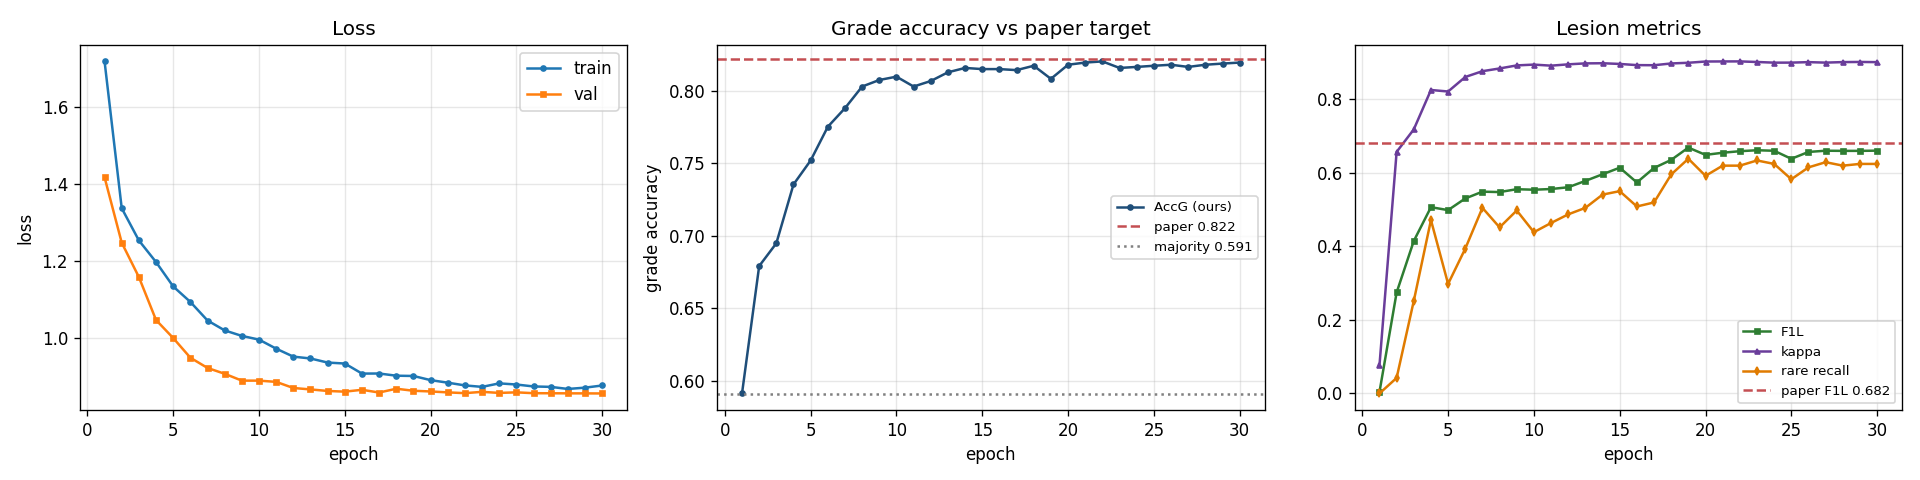
\includegraphics[width=\columnwidth]{exp2-curves.png}}
\caption{Experiment~II training dynamics over $30$ epochs. Left: training and validation
loss decrease monotonically ($1.718\!\rightarrow\!0.876$ and
$1.417\!\rightarrow\!0.856$) with no divergence, indicating the model was still improving
at the end of the schedule. Centre: validation grade accuracy rises from the majority
baseline ($0.591$, dotted) to $0.820$, converging on the published target ($0.822$,
dashed). Right: lesion macro-F1, quadratic $\kappa$, and mean rare-class recall.}
\label{fig:exp2_curves}
\end{figure}

\begin{figure}[!t]
\centerline{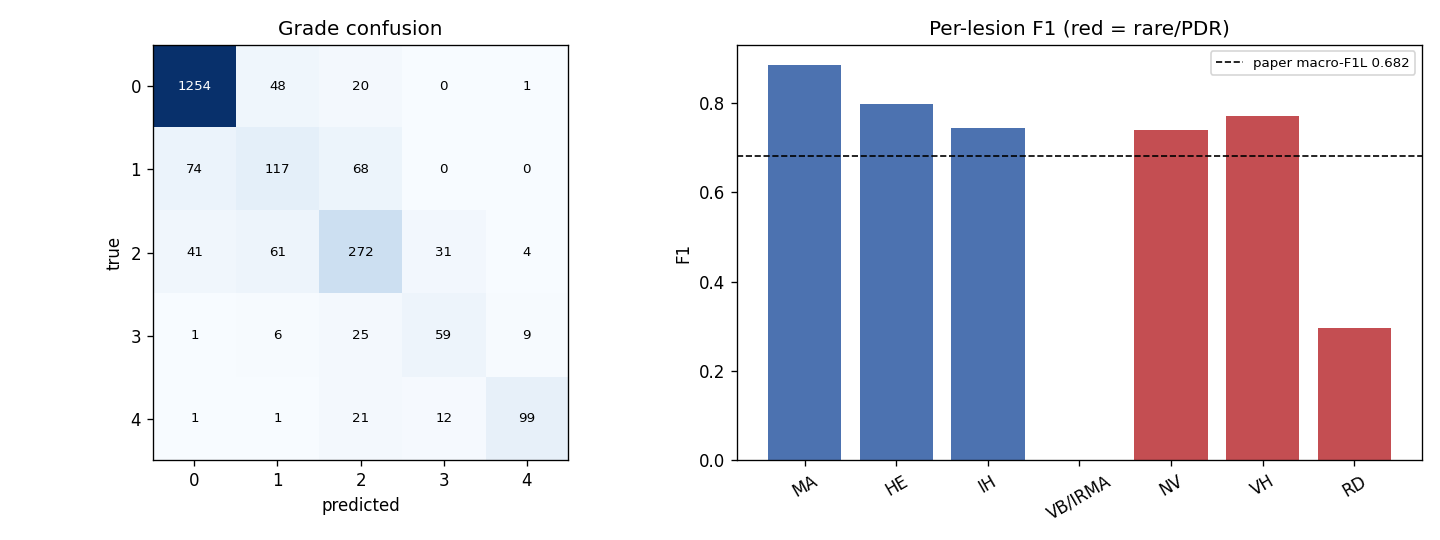
\includegraphics[width=\columnwidth]{exp2-breakdown.png}}
\caption{Experiment~II test-set breakdown. Left: the grade confusion matrix is strongly
near-diagonal, consistent with quadratic $\kappa=0.884$; the dominant residual error is
grade~1 being absorbed by its neighbours (recall $0.452$). Right: per-lesion F1 against
the published macro-F1 ($0.682$, dashed), with the rare PDR lesions in red. VB/IRMA
scores exactly zero at a $0.5$ threshold despite an AUROC of $0.949$, which alone costs
roughly $0.10$ of the seven-class macro average.}
\label{fig:exp2_breakdown}
\end{figure}

\subsection{Analysis}
The gap in lesion macro-F1 is a threshold-calibration effect, not a representational
failure. Two lesions dominate it: VB/IRMA scores $0.000$ and RD scores $0.296$ at a fixed
$0.5$ threshold, yet their AUROC values are $0.949$ and $0.994$ respectively---the model
ranks these cases almost perfectly but assigns them probabilities that never exceed
$0.5$, which is the expected behaviour of an unweighted BCE objective on classes with $43$
and $21$ test positives. Because a single zero enters a seven-class macro average
directly, VB/IRMA alone accounts for about $0.10$ of the shortfall. Fitting per-lesion
thresholds on the validation split recovers macro-F1 to $0.6743$, within one standard
error of the published value, without retraining. On the grading task the residual error
is concentrated in grade~1 (recall $0.452$), which is the clinically ambiguous mild-DR
category and the usual source of disagreement even between human graders.

\subsection{Discussion}
The reproduction supports the published claim that a retina-specific foundation model
performs strongly on MMRDR-CFP, and it locates the earlier contradictory result in a
software defect rather than in the method. Three factors were necessary: loading the
weights through a framework whose naming matches the checkpoint, training at the
published $512\times512$ resolution, and fine-tuning the full network with layer-wise
learning-rate decay instead of a hard freeze. The headline row deliberately retains
unweighted losses and a fixed $0.5$ threshold, because both published targets are
accuracy metrics and reweighting would raise macro-F1 while lowering accuracy, making the
comparison unreadable; the tuned-threshold row is reported separately as the better
clinical operating point.

\subsection{Limitations}
The result is single-seed, so no variance estimate accompanies it. Validation loss was
still decreasing at epoch~$30$, indicating the schedule ended before convergence and a
longer budget would likely add a small amount. Lesion macro-F1 at the fixed threshold
remains below the published value, and the ambiguity of which F1 averaging the source
paper used is unresolved, so all variants are recorded in the results file. Because this
experiment uses the official partition with a genuine held-out test set while
Experiments~I and~III use random splits in which validation doubles as test, its accuracy
is \emph{not} directly comparable to theirs despite the superficially similar magnitude.

\subsection{Conclusion}
Correcting a silent weight-loading failure and adopting the published protocol raises
RETFound's CFP grade accuracy from $66.50\%$ to $80.94\%$ and reproduces three of the four
published baseline metrics within their $95\%$ confidence intervals, with the fourth
recovered to $0.674$ once per-lesion thresholds are calibrated. The experiment also
demonstrates that a foundation-model transfer result is uninterpretable unless the weight
transfer itself is explicitly verified.

% ===========================================================================
\section{Experiment III: Feature-Pyramid Network with Spatial Attention on UWF}
\label{sec:exp3}

\subsection{Objective}
Experiment~III adapts the multi-task grading-and-lesion formulation to the
ultra-widefield (UWF) modality using a feature-pyramid network~\cite{fpn} with a
spatial-attention module~\cite{cbam}, predicting the DR grade and the seven-way
lesion vector from UWF images.

\subsection{Motivation}
UWF imaging captures up to $200^{\circ}$ of the retina and reveals peripheral
pathology that standard fundus photography misses, which is especially relevant
to the sight-threatening lesions of proliferative DR. Peripheral lesions are
small relative to the wide field, motivating an explicit multi-scale feature
pyramid and a spatial-attention gate to focus on informative regions. UWF images
also carry eyelid and eyelash artifacts at the field boundary, which require a
modality-specific mask.

\subsection{Methodology}
The approach couples a ResNet-50 backbone with a top-down feature pyramid that
aligns features across scales, followed by a spatial-attention module on the
highest-resolution fused map and two task heads. Both heads are trained with
focal losses to counter class imbalance.

\subsection{Experimental Setup}
The experiment was implemented in PyTorch and trained on a single CUDA GPU with
AMP and gradient accumulation. Model selection used validation grade accuracy with
early stopping.

\subsection{Dataset}
The UWF subset (\texttt{MMRDR-UWF/UWF.csv}) contains $10{,}404$ images. An 80/20
split with \texttt{random\_state}~$=42$ (random, not stratified) yields
$8{,}323$ training and $2{,}081$ validation images, the latter used
as the evaluation set. Grade and lesion imbalance are handled by the focal-loss
objectives.

\subsection{Preprocessing}
UWF images are masked with an elliptical field-of-view crop, \texttt{apply\_uwf\_mask}
(\texttt{tightness}~$=0.98$): the largest external contour is fitted with an
ellipse and pixels outside it are zeroed, removing eyelid and eyelash artifacts.
Images are resized to $1024\times1024$ to preserve small peripheral lesions and
normalised with ImageNet statistics. Training augmentation comprises random
horizontal and vertical flips, random rotation ($\pm15^{\circ}$), and mild colour
jitter; the validation transform applies only the mask, resize, and normalisation.

\subsection{Architecture}
The network \texttt{UWF\_MultiScaleDRNet} uses a ResNet-50 backbone split into its
stem and residual stages \texttt{layer1}--\texttt{layer4}. Four $1\times1$ lateral
convolutions project all stages to a common $512$-channel width, and a top-down
pathway with bilinear upsampling fuses them into a high-resolution map (the
feature-pyramid design~\cite{fpn}). A spatial-attention module~\cite{cbam}
(channel avg/max pooling followed by a $7\times7$ convolution and a sigmoid gate)
reweights this map to emphasise informative regions. After global average pooling,
two linear heads produce the lesion ($512\!\rightarrow\!7$) and grade
($512\!\rightarrow\!5$) predictions.

\subsection{Training Procedure}
Training was scheduled for up to $50$ epochs with early stopping (patience $8$) on
validation grade accuracy. It stopped at epoch $28$, with the best model at
\textbf{epoch~20}. AMP with gradient scaling and gradient-norm clipping at $1.0$
were used; a small physical batch was compensated by gradient accumulation.

\subsection{Hyperparameters}
Table~\ref{tab:exp3_hyper} lists the configuration.

\begin{table}[!t]
\caption{Experiment~III --- Training Configuration}
\label{tab:exp3_hyper}
\centering
\setlength{\tabcolsep}{5pt}
\begin{tabular}{|l|l|}
\hline
\textbf{Setting} & \textbf{Value} \\
\hline
Backbone & ResNet-50 + FPN + spatial attention \\
Input resolution & $1024\times1024$ \\
Field-of-view mask & Elliptical (\texttt{tightness}~$=0.98$) \\
Optimiser & AdamW \\
Learning rate & $3\times10^{-4}$ (constant) \\
Weight decay & $1\times10^{-4}$ \\
Batch size & $4$ (grad.\ accum.\ $6$ $\rightarrow$ eff.\ $24$) \\
Gradient clipping & max-norm $1.0$ \\
Mixed precision & Enabled (AMP) \\
Grade loss & Focal ($\alpha{=}1,\gamma{=}2$) \\
Lesion loss & Focal ($\alpha{=}0.25,\gamma{=}2$) ($\times1.5$) \\
Epochs (planned / run) & $50$ / $28$ (early stop, patience $8$) \\
Best epoch & $20$ \\
\hline
\end{tabular}
\end{table}

\subsection{Evaluation Metrics}
Top-1 grade accuracy and element-wise multi-label lesion accuracy (threshold
$0.5$) are recorded each epoch.

\subsection{Results}
The best validation grade accuracy is \textbf{0.7448} (74.48\%) at epoch~20, and
element-wise lesion accuracy peaks at $0.9066$ at epoch~25.
Table~\ref{tab:exp3_res} summarises the headline figures.
Fig.~\ref{fig:exp3_curves} shows the training trajectories,
Fig.~\ref{fig:exp3_samples} shows masked UWF training samples with their grade and
lesion labels, and Fig.~\ref{fig:exp3_cam} shows Grad-CAM attributions from the
spatial-attention layer.

\begin{table}[!t]
\caption{Experiment~III --- Best Validation Results}
\label{tab:exp3_res}
\centering
\setlength{\tabcolsep}{5pt}
\begin{tabular}{|l|c|c|}
\hline
\textbf{Metric} & \textbf{Best value} & \textbf{Epoch} \\
\hline
Grade accuracy & $0.7448$ & $20$ \\
Lesion accuracy (element-wise) & $0.9066$ & $25$ \\
\hline
\end{tabular}
\end{table}

\begin{figure}[!t]
\centerline{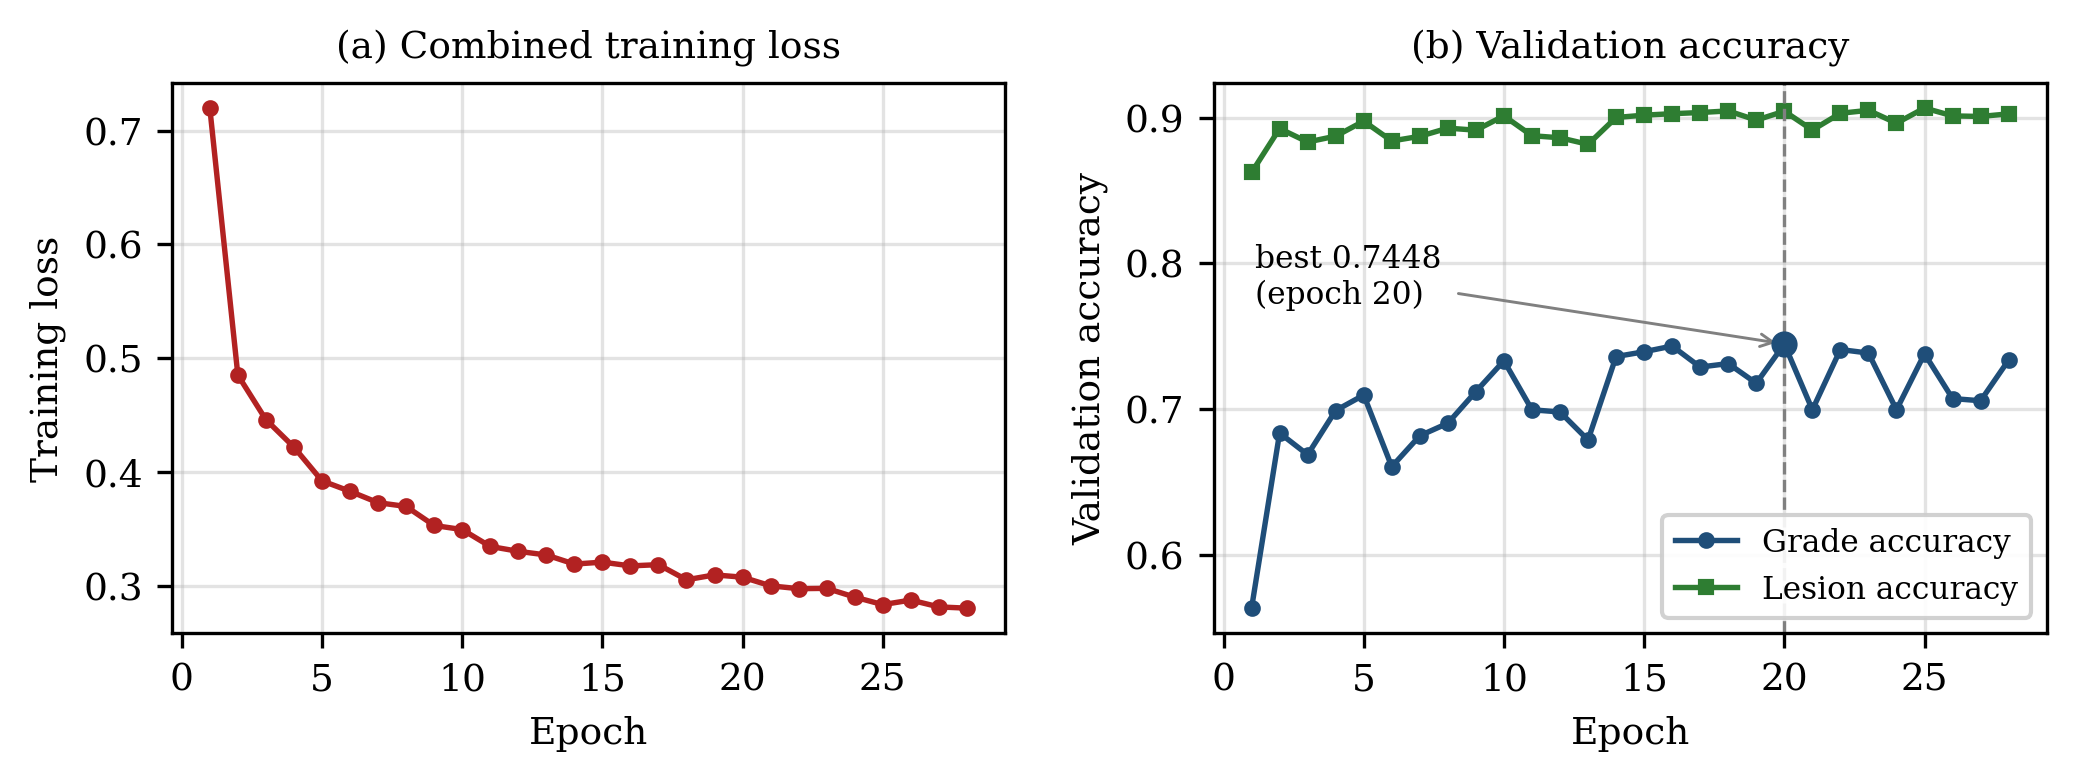
\includegraphics[width=\columnwidth]{exp3-training-curves.png}}
\caption{Experiment~III training dynamics. (a)~The combined training loss
decreases from $0.720$ to $0.281$ over $28$ epochs. (b)~Validation grade accuracy
fluctuates and peaks at $0.7448$ at epoch~20 (dashed line); element-wise lesion
accuracy remains near $0.90$. The oscillation reflects the small physical batch
and the noisy validation split.}
\label{fig:exp3_curves}
\end{figure}

\begin{figure*}[!t]
\centerline{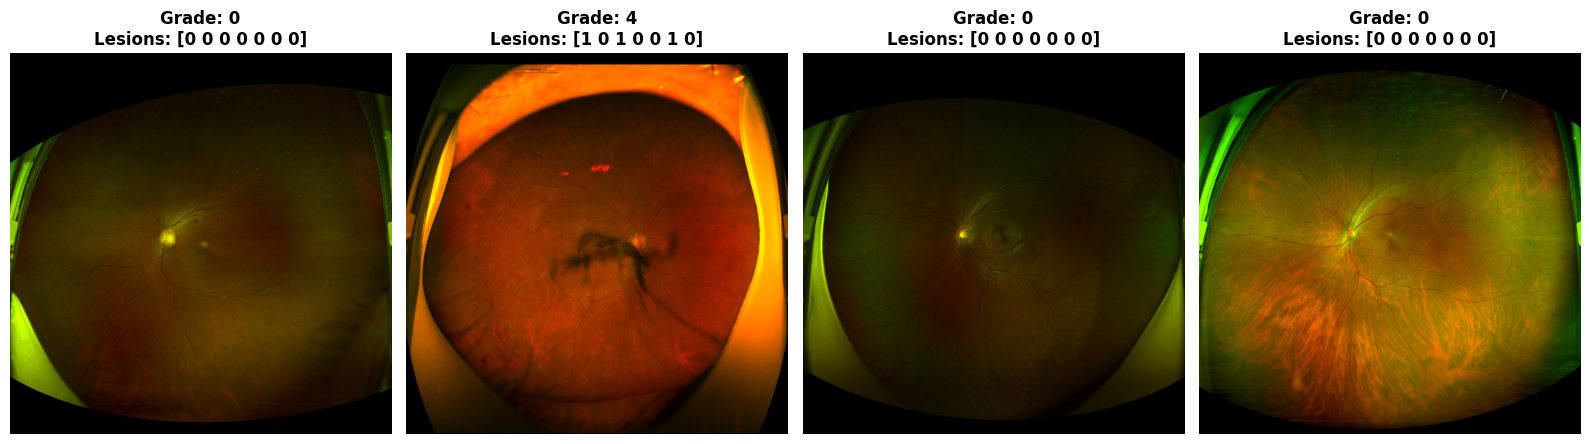
\includegraphics[width=0.95\textwidth]{exp3-samples.png}}
\caption{Masked UWF training samples (\texttt{apply\_uwf\_mask},
\texttt{tightness}~$=0.98$). Each panel shows the elliptical field-of-view crop
that removes eyelid/eyelash artifacts, annotated with the DR grade and the
seven-element multi-label lesion vector.}
\label{fig:exp3_samples}
\end{figure*}

\begin{figure}[!t]
\centerline{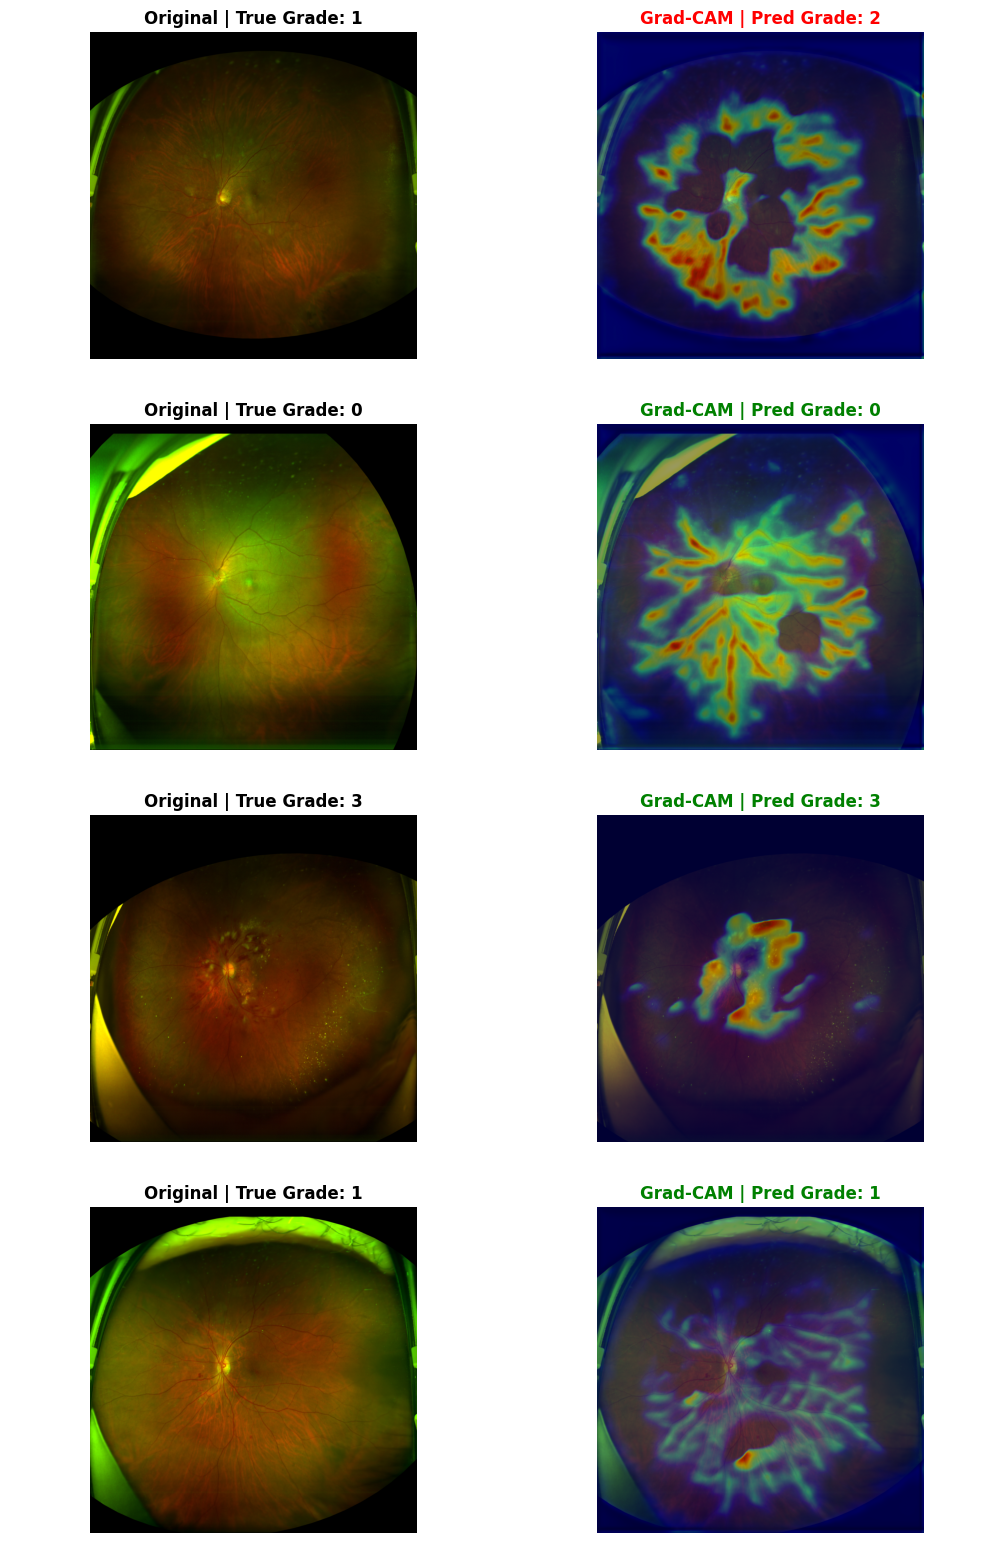
\includegraphics[width=\columnwidth]{exp3-gradcam.png}}
\caption{Grad-CAM~\cite{gradcam} attributions for \texttt{UWF\_MultiScaleDRNet},
computed at the spatial-attention layer. Each row shows a UWF image (left) and its
grade-head activation map (right), with the header green when the grade prediction
is correct and red when incorrect. Attention concentrates on the vascular arcades
and peripheral retina rather than the masked background.}
\label{fig:exp3_cam}
\end{figure}

\subsection{Analysis}
The training loss falls smoothly, but validation grade accuracy oscillates within
roughly $0.70$--$0.74$, with the optimum at epoch~20 ($0.7448$); the oscillation
is consistent with the small physical batch size ($4$) and the random, unstratified
validation split. Lesion accuracy stays high and stable ($\sim0.90$). The Grad-CAM
maps in Fig.~\ref{fig:exp3_cam} show attention concentrated on the vasculature and
peripheral retina, confirming that the spatial-attention pyramid attends to
plausible structures within the masked field of view.

\subsection{Discussion}
The feature-pyramid-plus-attention design adapts the multi-task formulation to the
wider, artifact-prone UWF field, and the $1024\times1024$ input with elliptical
masking preserves peripheral detail. Its best grade accuracy of $0.7448$ is below
the CFP convolutional baseline (Experiment~I), which is consistent with the greater
difficulty of UWF---a larger field, boundary artifacts, and a smaller effective
batch. The interpretable attention maps make it a useful UWF-specific reference.

\subsection{Limitations}
The validation grade accuracy is noisy because of the small physical batch and the
random, unstratified split, and the validation partition doubles as the evaluation
set. No global random seed is fixed, and the lesion-class semantics are not tracked
within the notebook.

\subsection{Conclusion}
The UWF feature-pyramid network with spatial attention attains a best validation
grade accuracy of $74.48\%$ while producing interpretable attention maps,
establishing the UWF reference baseline in this study.

% ===========================================================================
\section{Experiment IV: Clinically-Weighted Loss for High-Risk Lesions (UWF)}
\label{sec:exp4}

\subsection{Objective}
Experiment~IV keeps the multi-scale dual-branch architecture of Experiment~I but
retargets it to the ultra-widefield modality and replaces the lesion objective with
a \emph{clinically-weighted} loss. The aim is to bias the seven-way lesion detector
toward the rare, sight-threatening lesions of proliferative DR without altering the
architecture.

\subsection{Motivation}
Inverse-frequency weighting alone treats rarity as the only reason to up-weight a
class, but two lesions of equal rarity are not of equal clinical consequence: a
missed retinal detachment (RD) or neovascularization (NV) can precede irreversible
vision loss, whereas a missed microaneurysm rarely changes management. This
experiment therefore combines statistical rarity with an explicit,
ophthalmologist-motivated risk ordering so that the loss reflects the cost of a
miss, not merely its frequency.

\subsection{Methodology}
For the seven lesion classes, an inverse-frequency weight
$w^{\mathrm{freq}}_c = 1/(f_c+\epsilon)$ is multiplied by a hand-set clinical-risk
multiplier $r_c$ and the product is normalised to unit mean:
\begin{equation}
w_c = \frac{w^{\mathrm{freq}}_c \, r_c}{\frac{1}{C}\sum_{k} w^{\mathrm{freq}}_k \, r_k},
\qquad r = [1,1,2,2,4,4,5].
\label{eq:hybrid}
\end{equation}
The resulting vector $w_c$ is supplied as the \texttt{pos\_weight} of a
\texttt{BCEWithLogitsLoss} for the lesion head, while the grade head uses standard
cross-entropy; the two are added with equal weight. The risk multipliers escalate
from common lesions (MA, HE $=1$) through intermediate ones (IH, cotton-wool spots
$=2$) to the PDR-defining lesions (NV, VH $=4$; RD $=5$).

\subsection{Experimental Setup}
The experiment was implemented in PyTorch and trained on a single CUDA GPU.
Model selection saved the checkpoint with the lowest validation loss, with early
stopping on the same criterion.

\subsection{Dataset}
The UWF subset (\texttt{MMRDR-UWF/UWF.csv}) is split 80/20 with
\texttt{random\_state}~$=42$ (random, not stratified), giving $8{,}323$ training and
$2{,}081$ validation images; the validation partition is used as the evaluation set.
The lesion frequencies mined from the training data---MA~$6938$, HE~$3846$,
IH~$3849$, CWS~$1010$, NV~$1188$, VH~$1219$, RD~$238$---drive the inverse-frequency
term of \eqref{eq:hybrid}.

\subsection{Preprocessing}
Images are masked with the elliptical field-of-view crop \texttt{apply\_uwf\_mask}
(\texttt{tightness}~$=0.98$), resized to $512\times512$, and normalised with
ImageNet statistics. Training augmentation applies random horizontal and vertical
flips, random rotation ($\pm15^{\circ}$), and mild colour jitter; validation applies
only the mask, resize, and normalisation.

\subsection{Architecture}
The network is \texttt{MultiScaleLesionAttentionNet} (Experiment~I): a ResNet-50
whose early, pre-maxpool features (at $256\times256$) preserve microaneurysm-scale
detail while the full trunk supplies global context; the two branches are
channel-aligned to $512\times16\times16$, summed, and split into a lesion head and a
grade head with dropout.

\subsection{Training Procedure}
Training was scheduled for $50$ epochs with early stopping (patience $8$) on
validation loss and a cosine-annealed learning rate
($1\times10^{-4}\!\rightarrow\!1\times10^{-6}$). It stopped at epoch $22$, with the
best (lowest-loss) checkpoint at \textbf{epoch~14}.

\subsection{Hyperparameters}
Table~\ref{tab:exp4_hyper} lists the configuration and the resulting normalised
lesion weights.

\begin{table}[!t]
\caption{Experiment~IV --- Training Configuration and Lesion Weights}
\label{tab:exp4_hyper}
\centering
\setlength{\tabcolsep}{5pt}
\begin{tabular}{|l|l|}
\hline
\textbf{Setting} & \textbf{Value} \\
\hline
Backbone & \texttt{MultiScaleLesionAttentionNet} \\
Input resolution & $512\times512$ \\
Field-of-view mask & Elliptical (\texttt{tightness}~$=0.98$) \\
Optimiser & Adam \\
Learning rate & $1\times10^{-4}$, cosine to $1\times10^{-6}$ \\
Batch size & $8$ \\
Grade loss & Cross-entropy \\
Lesion loss & BCE with clinical \texttt{pos\_weight} \\
Epochs (planned / run) & $50$ / $22$ (early stop, patience $8$) \\
Best epoch & $14$ (lowest val loss) \\
\hline
\multicolumn{2}{|c|}{\textbf{Normalised lesion weights} $w_c$ (mean $=1$)} \\
\hline
MA / HE / IH & $0.033$ / $0.060$ / $0.119$ \\
CWS / NV / VH & $0.454$ / $0.771$ / $0.752$ \\
RD & $4.812$ \\
\hline
\end{tabular}
\end{table}

\subsection{Evaluation Metrics}
The best checkpoint is evaluated on the validation set with grade accuracy and a
full per-class classification report (precision, recall, F1) for both the five
grades and the seven lesions at a $0.5$ decision threshold.

\subsection{Results}
The best checkpoint reaches a grade accuracy of \textbf{76.50\%} (grade macro-F1
$0.75$). The clinical weighting has its intended effect on the lesion head: the
highest-risk lesions are recalled well despite their rarity---RD recall $0.79$
(support $48$), VH $0.77$, NV $0.68$---while the down-weighted common lesions HE and
CWS collapse to recall $0.10$ and $0.04$. Precision remains high throughout, so the
lesion macro-F1 ($0.56$) is limited by recall on the intentionally de-emphasised
classes rather than by false positives. Table~\ref{tab:exp4_res} reports the
per-lesion breakdown and Fig.~\ref{fig:exp4_curves} the loss trajectory.

\begin{table}[!t]
\caption{Experiment~IV --- Per-Lesion Validation Performance (Best Checkpoint)}
\label{tab:exp4_res}
\centering
\setlength{\tabcolsep}{5pt}
\begin{tabular}{|l|c|c|c|c|}
\hline
\textbf{Lesion} & \textbf{Prec.} & \textbf{Recall} & \textbf{F1} & \textbf{Support} \\
\hline
MA & $1.00$ & $0.72$ & $0.83$ & $1388$ \\
HE & $1.00$ & $0.10$ & $0.19$ & $780$ \\
IH & $0.94$ & $0.36$ & $0.52$ & $741$ \\
CWS & $0.50$ & $0.04$ & $0.07$ & $193$ \\
NV & $0.88$ & $0.68$ & $0.76$ & $238$ \\
VH & $0.98$ & $0.77$ & $0.86$ & $226$ \\
RD & $0.63$ & $0.79$ & $0.70$ & $48$ \\
\hline
Macro avg & $0.85$ & $0.49$ & $0.56$ & $3614$ \\
Micro avg & $0.96$ & $0.48$ & $0.64$ & $3614$ \\
\hline
\multicolumn{5}{|l|}{Grade accuracy $=0.7650$; grade macro-F1 $=0.75$.} \\
\hline
\end{tabular}
\end{table}

\begin{figure}[!t]
\centerline{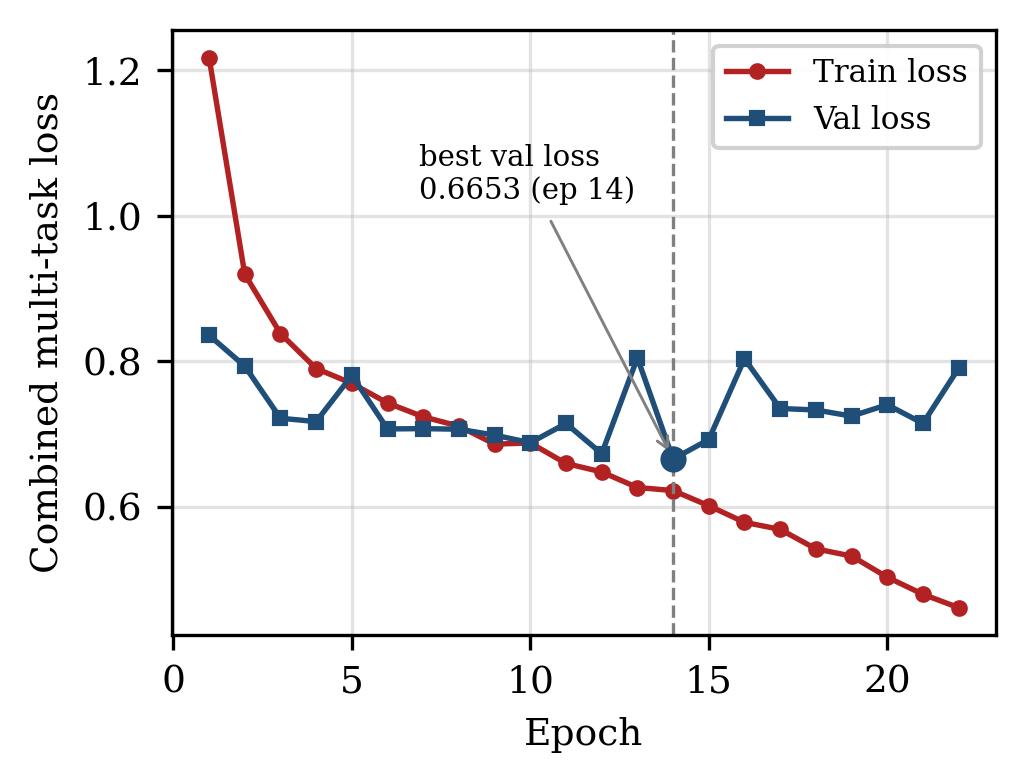
\includegraphics[width=\columnwidth]{exp4-training-curves.png}}
\caption{Experiment~IV training dynamics. The combined training loss decreases
monotonically while the validation loss reaches its minimum ($0.6653$) at epoch~14
(dashed line) and then rises, triggering early stopping at epoch~22. The
best-validation-loss checkpoint from epoch~14 is the one evaluated in
Table~\ref{tab:exp4_res}.}
\label{fig:exp4_curves}
\end{figure}

\subsection{Analysis}
The experiment demonstrates a controllable trade-off: by encoding clinical risk
directly in \eqref{eq:hybrid}, recall is redistributed toward the PDR-defining
lesions (NV, VH, RD) at the deliberate expense of the common, low-risk lesions.
This is the desired behaviour for a screening tool whose dominant failure mode
should be over-referral rather than a missed proliferative case. Grade accuracy
($76.50\%$) is on par with the plain UWF baseline of Experiment~III ($74.48\%$),
indicating that the lesion re-weighting did not degrade grading.

\subsection{Discussion}
Relative to the plain UWF baseline, the clinically-weighted loss changes
\emph{which} lesions the model prioritises rather than the overall grade accuracy.
The very large normalised weight on RD ($4.81$) is effective but also the reason
common-lesion recall drops sharply; the risk multipliers are a design lever that
could be tuned to a target operating point. The consistently high precision shows
the model stays conservative, which is appropriate for the rare classes but leaves
headroom on recall for the mid-risk lesions.

\subsection{Limitations}
The best model is selected on validation loss, and the validation split doubles as
the evaluation set; the split is random and unstratified, and no global seed is
fixed. The risk multipliers are hand-set rather than calibrated to a clinical
utility function. The lesion index~$3$ is labelled ``CWS'' (cotton-wool spots) in
this notebook, whereas the dataset schema names that position VB/IRMA; the numeric
targets are unaffected, but the semantic label differs from the other experiments.

\subsection{Conclusion}
Encoding clinical risk into the lesion loss steers a UWF multi-task model toward
detecting the sight-threatening lesions of proliferative DR (RD recall $0.79$,
VH $0.77$, NV $0.68$) while maintaining a grade accuracy of $76.50\%$, at the
intended cost of recall on common lesions.

% ===========================================================================
\section{Experiment V: Asymmetric False-Negative-Penalised Loss (UWF)}
\label{sec:exp5}

\subsection{Objective}
Experiment~V targets the same rare-lesion problem from the loss side, replacing the
lesion objective of the UWF feature-pyramid network with an \emph{asymmetric focal
loss} that penalises false negatives on the PDR-defining lesions far more heavily
than false positives.

\subsection{Motivation}
For proliferative DR, a false negative---reassuring a patient who in fact has
neovascularization, vitreous haemorrhage, or retinal detachment---can lead to
irreversible blindness, whereas a false positive merely prompts an unnecessary
follow-up. Symmetric objectives such as binary cross-entropy treat the two errors
identically, which is clinically inappropriate. The asymmetric loss makes the cost
of a miss explicit and lesion-specific~\cite{asl,focalloss}.

\subsection{Methodology}
The loss modulates the focal loss with a per-class positive weight $\beta_c$:
\begin{equation}
L_{\mathrm{asym}} =
\begin{cases}
\beta_c\,(1-p_t)^{\gamma}\,\mathrm{BCE}, & y=1 \ (\text{miss penalty})\\[2pt]
(1-\beta_c)\,(1-p_t)^{\gamma}\,\mathrm{BCE}, & y=0 \ (\text{false-alarm penalty})
\end{cases}
\label{eq:asym}
\end{equation}
with $\gamma=2$ and $\beta = [0.7,0.7,0.7,0.8,0.95,0.95,0.95]$ over
$[\text{MA},\text{HE},\text{IH},\text{VB/IRMA},\text{NV},\text{VH},\text{RD}]$, so
the three PDR lesions (indices $4$--$6$) carry $\beta=0.95$. A built-in check
confirms the asymmetry: for the same confidence, missing an NV lesion incurs loss
$0.2536$ versus $0.0415$ for hallucinating one---roughly a sixfold penalty. The
grade head uses cross-entropy, added with equal weight.

\subsection{Experimental Setup}
Implemented in PyTorch on a single CUDA GPU with automatic mixed precision and
gradient-norm clipping. Grade quality is monitored with a quadratic-weighted
Cohen's~$\kappa$ (which credits near-diagonal ordinal errors) alongside accuracy,
and lesion quality with a macro-averaged F1 and AUC.

\subsection{Dataset}
The UWF subset is split 80/20 with \texttt{random\_state}~$=42$ (random, not
stratified): $8{,}323$ training and $2{,}081$ validation images, the latter used for
evaluation.

\subsection{Preprocessing}
Each image is resized to $512\times512$ before the elliptical
\texttt{apply\_uwf\_mask} (\texttt{tightness}~$=0.98$) is applied---resizing first
keeps the heavy OpenCV masking from bottlenecking the data loader---and normalised
with ImageNet statistics. Training augmentation uses random horizontal/vertical
flips, colour jitter, and random rotation ($\pm10^{\circ}$); validation applies only
the resize, mask, and normalisation.

\subsection{Architecture}
The network is \texttt{UWF\_MultiScaleDRNet}: a ResNet-50 backbone with four
$1\times1$ lateral convolutions and a top-down, bilinearly-upsampled feature
pyramid~\cite{fpn}, a $7\times7$ spatial-attention gate~\cite{cbam} on the fused
map, global average pooling, a $50\%$ dropout layer, and two linear heads for the
seven lesions and five grades. Relative to Experiment~III the input is
$512\times512$ (rather than $1024\times1024$) and an explicit dropout layer is added
for regularisation.

\subsection{Training Procedure}
Training was scheduled for up to $100$ epochs with early stopping (patience $15$) on
validation loss and a \texttt{ReduceLROnPlateau} schedule (factor $0.5$, patience
$3$) that stepped the learning rate down at epochs $15$, $21$, $25$, and $29$.
Training stopped at epoch $31$, with the best (lowest-loss) checkpoint at
\textbf{epoch~16}.

\subsection{Hyperparameters}
Table~\ref{tab:exp5_hyper} lists the configuration.

\begin{table}[!t]
\caption{Experiment~V --- Training Configuration}
\label{tab:exp5_hyper}
\centering
\setlength{\tabcolsep}{5pt}
\begin{tabular}{|l|l|}
\hline
\textbf{Setting} & \textbf{Value} \\
\hline
Backbone & ResNet-50 + FPN + spatial attention + dropout \\
Input resolution & $512\times512$ \\
Field-of-view mask & Elliptical (\texttt{tightness}~$=0.98$) \\
Optimiser & AdamW \\
Learning rate & $1\times10^{-4}$ (\texttt{ReduceLROnPlateau}) \\
Weight decay & $1\times10^{-3}$ \\
Batch size & $8$ \\
Gradient clipping & max-norm $2.0$ \\
Mixed precision & Enabled (AMP) \\
Grade loss & Cross-entropy \\
Lesion loss & Asymmetric focal ($\gamma{=}2$; $\beta$ per class) \\
Epochs (planned / run) & $100$ / $31$ (early stop, patience $15$) \\
Best epoch & $16$ (lowest val loss) \\
\hline
\end{tabular}
\end{table}

\subsection{Evaluation Metrics}
Each epoch records grade accuracy, quadratic-weighted Cohen's~$\kappa$, and
macro-averaged lesion F1 and AUC on the validation set.

\subsection{Results}
At the best-validation-loss checkpoint (epoch~16) the model attains grade accuracy
\textbf{0.7578}, quadratic $\kappa$ \textbf{0.9208}, lesion macro-F1 $0.7151$, and
lesion AUC $0.9504$. Grade accuracy continues to rise afterward---peaking at
$0.7770$ (epoch~22) with $\kappa=0.9304$---but the validation loss is already
increasing, so the checkpoint policy retains epoch~16. Lesion AUC is stable near
$0.95$ throughout and lesion F1 peaks at $0.7311$ (epoch~31).
Table~\ref{tab:exp5_res} lists the selected-checkpoint and peak values, and
Fig.~\ref{fig:exp5_curves} shows the trajectories.

\begin{table}[!t]
\caption{Experiment~V --- Validation Results}
\label{tab:exp5_res}
\centering
\setlength{\tabcolsep}{5pt}
\begin{tabular}{|l|c|c|}
\hline
\textbf{Metric} & \textbf{Epoch 16 (selected)} & \textbf{Best (epoch)} \\
\hline
Grade accuracy & $0.7578$ & $0.7770$ ($22$) \\
Grade $\kappa$ (quad.) & $0.9208$ & $0.9313$ ($25$) \\
Lesion macro-F1 & $0.7151$ & $0.7311$ ($31$) \\
Lesion macro-AUC & $0.9504$ & $0.9507$ ($26$) \\
\hline
\end{tabular}
\end{table}

\begin{figure}[!t]
\centerline{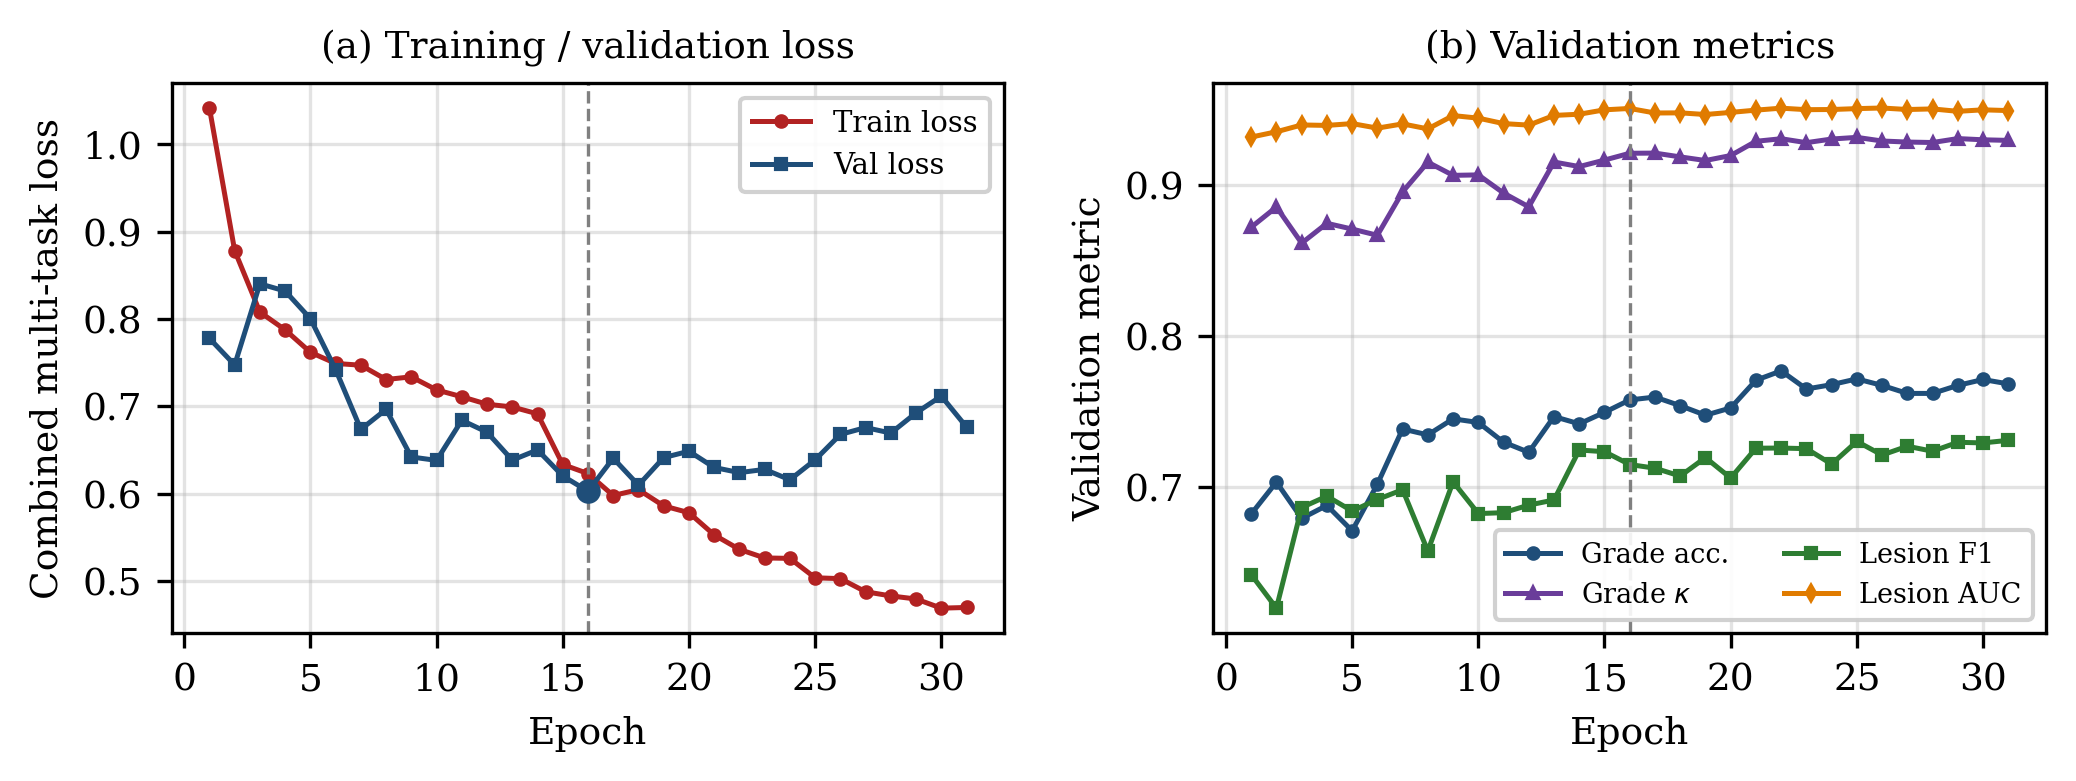
\includegraphics[width=\columnwidth]{exp5-training-curves.png}}
\caption{Experiment~V training dynamics over $31$ epochs. (a)~Training loss falls
steadily while validation loss bottoms out at epoch~16 (dashed line) and then
diverges---classic overfitting captured by the checkpoint policy. (b)~Validation
grade accuracy and quadratic $\kappa$ climb into the high-$0.9$ range for $\kappa$,
while lesion AUC holds near $0.95$; the asymmetric loss yields strong ordinal grade
agreement and stable lesion ranking.}
\label{fig:exp5_curves}
\end{figure}

\begin{figure*}[!t]
\centerline{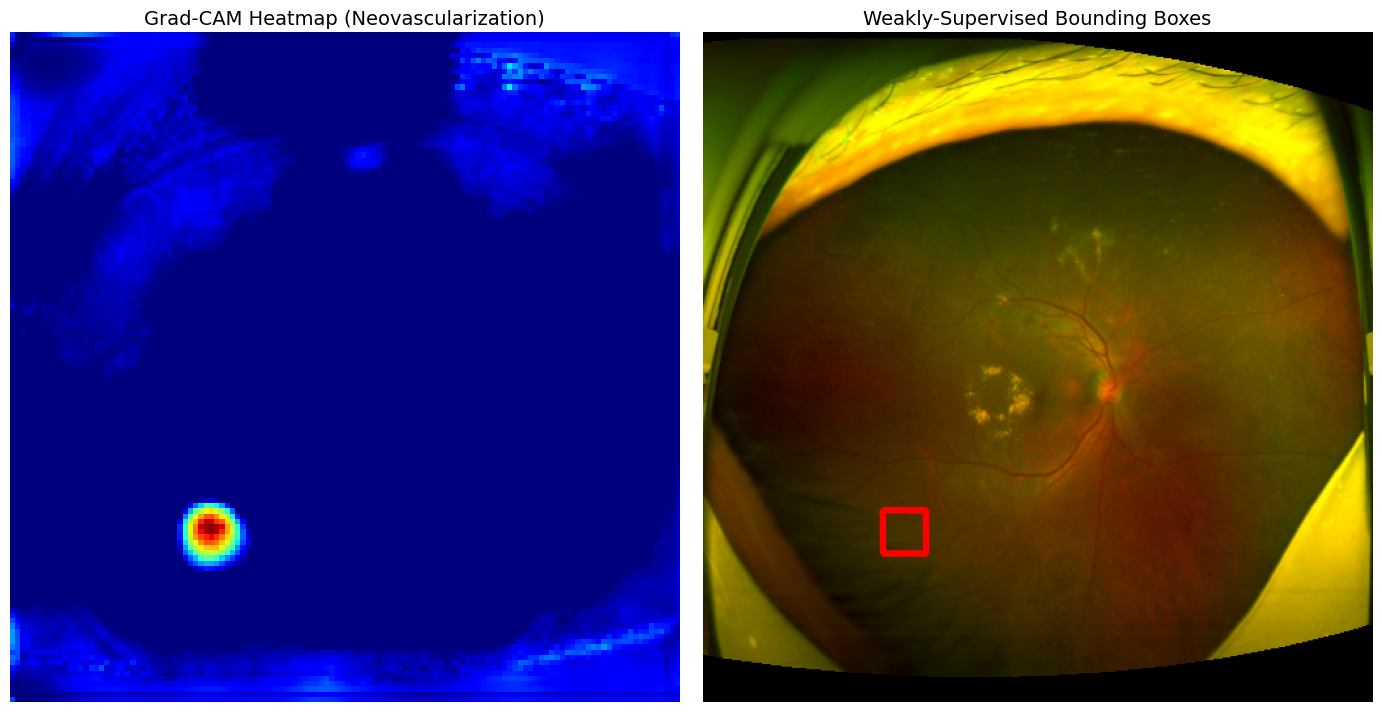
\includegraphics[width=0.95\textwidth]{exp5-gradcam.png}}
\caption{Weakly-supervised localization for \texttt{UWF\_MultiScaleDRNet}. Because
the dataset has no bounding-box annotations, a Grad-CAM~\cite{gradcam} heatmap for
the neovascularization (NV) logit (left) is thresholded to derive a bounding box
(right). The activation concentrates on a focal region of the masked retina,
illustrating how the FN-penalised model can be used for approximate lesion
localization without box labels.}
\label{fig:exp5_cam}
\end{figure*}

\subsection{Analysis}
The asymmetric objective produces a strong ordinal grader---quadratic $\kappa$
around $0.92$ means most grade errors fall on adjacent severities---and a
well-ranked lesion detector (AUC $\approx0.95$). The divergence between training and
validation loss after epoch~16 shows the model begins to overfit the small,
unstratified validation split, which the early-stopping-on-loss policy handles
correctly.

\subsection{Discussion}
Compared with the frequency-and-risk weighting of Experiment~IV, the asymmetric
loss encodes the miss/false-alarm asymmetry more directly and yields a higher
overall lesion macro-F1 ($0.715$ vs.\ $0.56$) because it does not suppress the
common lesions as aggressively. The lower input resolution ($512$ vs.\ $1024$ in
Experiment~III) trades peripheral detail for a larger effective batch and faster
epochs while retaining strong grade agreement.

\subsection{Limitations}
The model is selected on validation loss and the validation partition doubles as the
evaluation set; the split is random and unstratified and no seed is fixed. The
best checkpoint was not retained on disk. The weakly-supervised bounding box is
illustrative and unvalidated against ground-truth lesion locations.

\subsection{Conclusion}
An asymmetric, false-negative-penalised focal loss trains the UWF feature-pyramid
network to a quadratic $\kappa$ of $0.92$ and lesion AUC of $0.95$ at a grade
accuracy of $75.8\%$, and its Grad-CAM maps support weakly-supervised lesion
localization without bounding-box labels.

% ===========================================================================
\section{Experiment VI: Supervised Contrastive Learning for Rare Lesions (UWF)}
\label{sec:exp6}

\subsection{Objective}
Experiment~VI attacks the rare-lesion problem in the \emph{representation} rather
than only the loss weighting, adding a supervised contrastive
objective~\cite{supcon} on intermediate features so that images containing PDR
lesions are pulled together and separated from those without.

\subsection{Motivation}
Loss re-weighting (Experiments~IV--V) adjusts the decision boundary but leaves the
feature space unchanged. If the embeddings of rare-lesion images are not already
well separated, the classifier must work against an entangled representation.
Supervised contrastive learning shapes the feature space directly, encouraging a
cluster for rare-lesion images that the linear heads can then read out more
reliably.

\subsection{Methodology}
A binary label---whether an image contains any of NV, VH, or RD---supervises a
contrastive loss applied at two depths: an ``early'' projection of the
\texttt{layer2} features and a ``deep'' projection of the \texttt{layer4} features,
each mapped by a two-layer MLP to a $128$-d embedding. The total objective is
\begin{equation}
L = L_{\mathrm{asym}} + L_{\mathrm{CE}}
  + 0.5\,L_{\mathrm{SupCon}}^{\mathrm{early}}
  + 0.5\,L_{\mathrm{SupCon}}^{\mathrm{deep}},
\label{eq:supcon}
\end{equation}
where $L_{\mathrm{asym}}$ is the asymmetric focal lesion loss of Experiment~V,
$L_{\mathrm{CE}}$ the grade cross-entropy, and each SupCon term uses temperature
$\tau=0.1$. Classification still flows through the FPN-fused map; the contrastive
heads act only as an auxiliary representational signal.

\subsection{Experimental Setup}
Implemented in PyTorch and trained across two CUDA GPUs with
\texttt{DataParallel}. The same accuracy, quadratic-$\kappa$, macro-F1, and AUC
metrics as Experiment~V are recorded each epoch.

\subsection{Dataset}
The UWF subset is split 80/20 with \texttt{random\_state}~$=42$ (random, not
stratified): $8{,}323$ training and $2{,}081$ validation images. The contrastive
label is derived per image as $\mathbb{1}[\text{NV}\lor\text{VH}\lor\text{RD}]$.

\subsection{Preprocessing}
Identical to Experiment~V: resize to $512\times512$, elliptical
\texttt{apply\_uwf\_mask} (\texttt{tightness}~$=0.98$), ImageNet normalisation, and
flip/colour-jitter/rotation ($\pm10^{\circ}$) augmentation on the training split
only.

\subsection{Architecture}
The network \texttt{UWF\_SupConDRNet} shares the ResNet-50 backbone and top-down
feature pyramid~\cite{fpn} with Experiment~V (without the spatial-attention gate)
and adds two projection heads: \texttt{proj\_early} ($512\!\rightarrow\!512\!
\rightarrow\!128$) on globally-pooled \texttt{layer2} features and
\texttt{proj\_deep} ($2048\!\rightarrow\!512\!\rightarrow\!128$) on \texttt{layer4}
features. The FPN-fused map is globally pooled and read out by linear lesion
($512\!\rightarrow\!7$) and grade ($512\!\rightarrow\!5$) heads.

\subsection{Training Procedure}
Training was scheduled for $60$ epochs with early stopping (patience $10$) on
validation loss and \texttt{ReduceLROnPlateau} (factor $0.5$, patience $3$), with
gradient-norm clipping at $2.0$. The captured run is a \emph{resumption} from a
checkpoint at epoch~$27$; it continued through epoch~$37$ and then early-stopped
because the validation loss never improved on the epoch-$27$ value---that is, the
model had already converged by epoch~$27$. Consequently the best-loss checkpoint
(the only preserved checkpoint on disk, \texttt{best\_model (for 3).pth}) predates
the captured log, and the metrics reported below characterise the converged plateau
of epochs $28$--$37$.

\subsection{Hyperparameters}
Table~\ref{tab:exp6_hyper} lists the configuration.

\begin{table}[!t]
\caption{Experiment~VI --- Training Configuration}
\label{tab:exp6_hyper}
\centering
\setlength{\tabcolsep}{5pt}
\begin{tabular}{|l|l|}
\hline
\textbf{Setting} & \textbf{Value} \\
\hline
Backbone & ResNet-50 + FPN + two SupCon heads \\
Compute & $2\times$ GPU (\texttt{DataParallel}) \\
Input resolution & $512\times512$ \\
Optimiser & AdamW \\
Learning rate & $1\times10^{-4}$ (\texttt{ReduceLROnPlateau}) \\
Weight decay & $1\times10^{-4}$ \\
Batch size & $8$ \\
Gradient clipping & max-norm $2.0$ \\
SupCon temperature & $\tau=0.1$ \\
Loss & Asym.\ focal $+$ CE $+ 0.5$ SupCon$_\text{early}$ $+ 0.5$ SupCon$_\text{deep}$ \\
Epochs (planned) & $60$ (early stop, patience $10$) \\
Captured run & Resumed epochs $28$--$37$ \\
\hline
\end{tabular}
\end{table}

\subsection{Evaluation Metrics}
Grade accuracy, quadratic-weighted Cohen's~$\kappa$, and macro-averaged lesion F1
and AUC, evaluated on the validation set each epoch.

\subsection{Results}
Over the converged plateau (epochs $28$--$37$) validation grade accuracy holds
between $0.7544$ and \textbf{0.7645} (peak at epoch~$31$), quadratic $\kappa$
between $0.9157$ and $0.9223$, lesion macro-F1 between $0.7243$ and $0.7390$, and
lesion macro-AUC between $0.9501$ and $0.9523$---the highest lesion AUC among the
UWF experiments. Training loss keeps falling while validation loss drifts slightly
upward (Fig.~\ref{fig:exp6_curves}), consistent with a converged model that is
beginning to overfit. Table~\ref{tab:exp6_res} reports the plateau ranges.
Fig.~\ref{fig:exp6_cam} shows Grad-CAM localization on a genuine rare-lesion case.

\begin{table}[!t]
\caption{Experiment~VI --- Validation Results (Converged Plateau, Epochs 28--37)}
\label{tab:exp6_res}
\centering
\setlength{\tabcolsep}{5pt}
\begin{tabular}{|l|c|c|}
\hline
\textbf{Metric} & \textbf{Plateau range} & \textbf{Peak (epoch)} \\
\hline
Grade accuracy & $0.754$--$0.765$ & $0.7645$ ($31$) \\
Grade $\kappa$ (quad.) & $0.916$--$0.922$ & $0.9223$ ($36$) \\
Lesion macro-F1 & $0.724$--$0.739$ & $0.7390$ ($29$) \\
Lesion macro-AUC & $0.950$--$0.952$ & $0.9523$ ($28$) \\
\hline
\multicolumn{3}{|l|}{Best-loss checkpoint predates the captured log (epoch $\le27$).}\\
\hline
\end{tabular}
\end{table}

\begin{figure}[!t]
\centerline{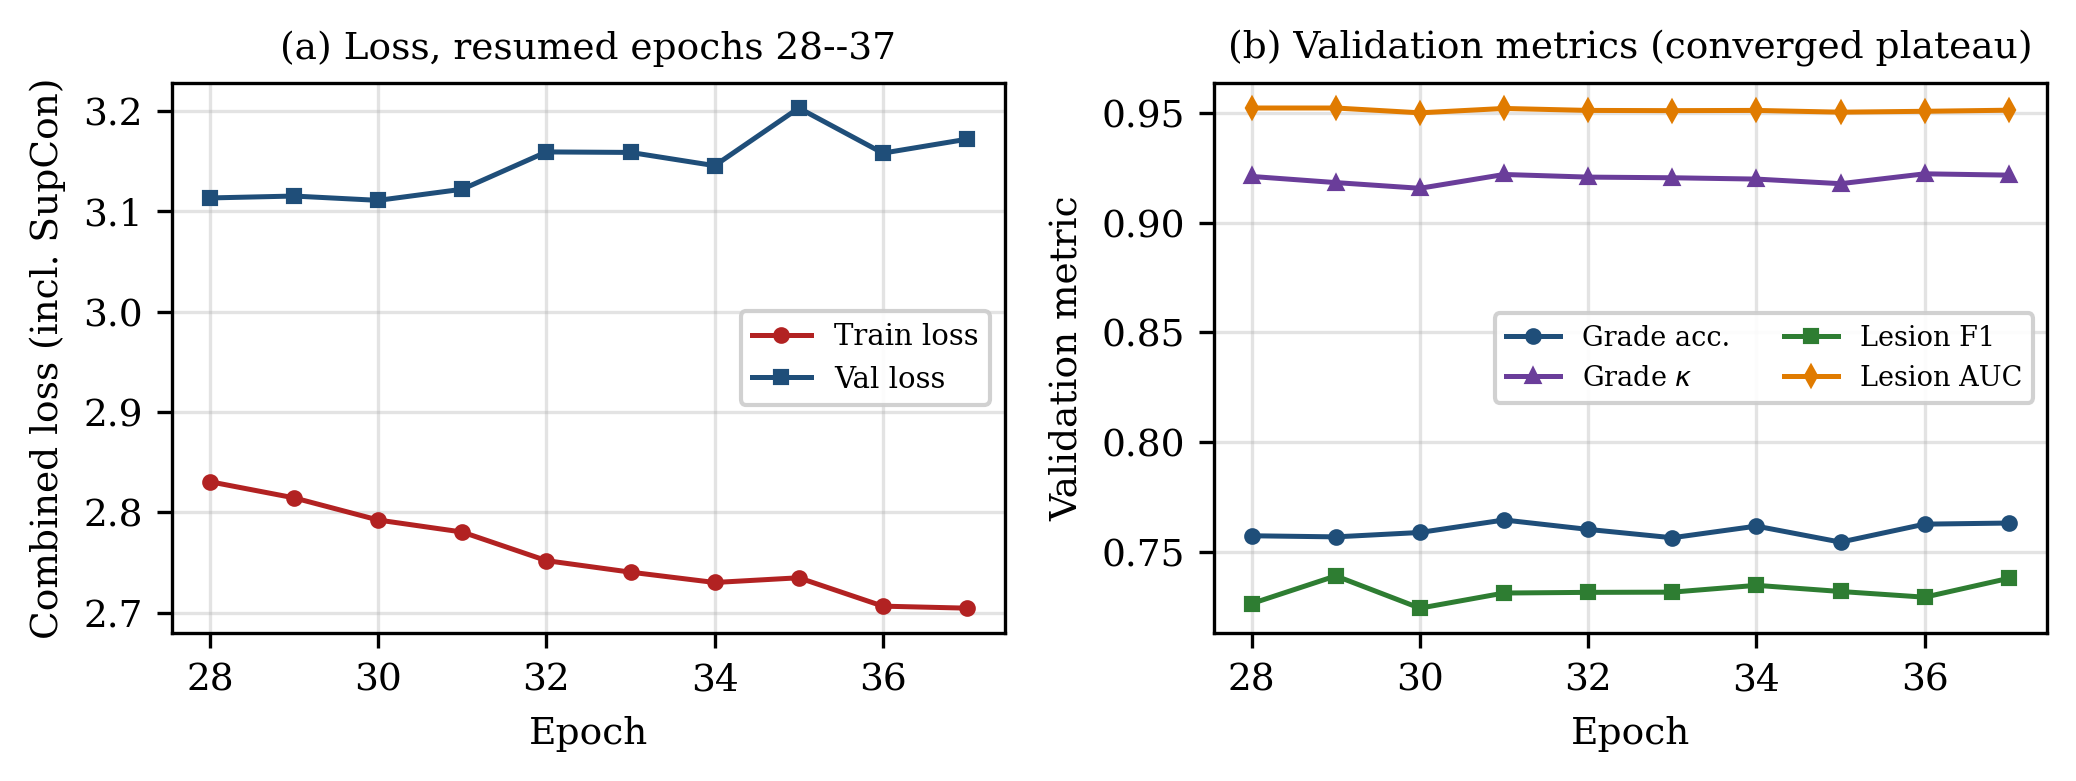
\includegraphics[width=\columnwidth]{exp6-training-curves.png}}
\caption{Experiment~VI training dynamics over the captured, resumed epochs
$28$--$37$. (a)~Training loss (which includes the two contrastive terms and is thus
not comparable in absolute value to the other experiments) continues to fall while
validation loss drifts upward. (b)~Validation grade accuracy, quadratic $\kappa$,
lesion F1, and AUC are essentially flat, confirming that the model had already
converged before the captured window.}
\label{fig:exp6_curves}
\end{figure}

\begin{figure}[!t]
\centerline{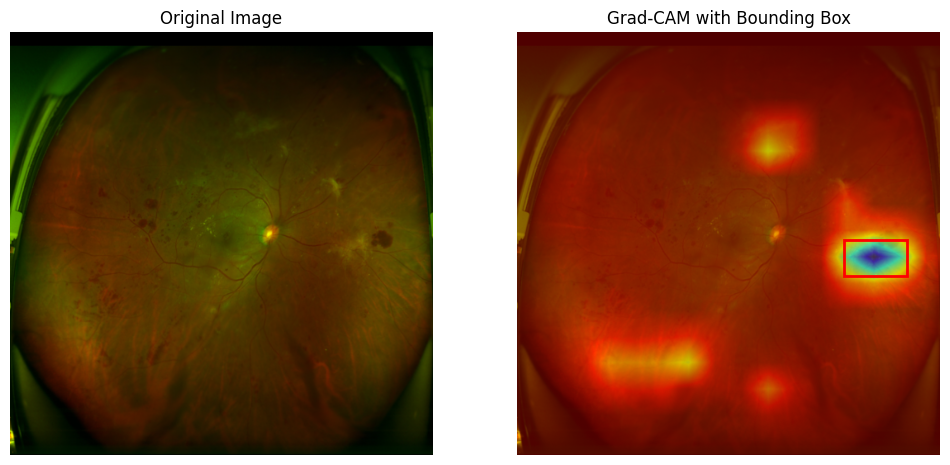
\includegraphics[width=\columnwidth]{exp6-gradcam.png}}
\caption{Grad-CAM~\cite{gradcam} localization for \texttt{UWF\_SupConDRNet} on a
validation image that genuinely contains a rare (NV) lesion. The heatmap is computed
at \texttt{layer4} for the NV logit and overlaid on the masked UWF image (right),
with a thresholded bounding box marking the peak activation. The contrastive
auxiliary yields focal activation on a plausible peripheral region.}
\label{fig:exp6_cam}
\end{figure}

\subsection{Analysis}
On the converged plateau the contrastive model matches the asymmetric-loss model on
grade accuracy and $\kappa$ and attains the highest lesion AUC of the UWF group
($\approx0.952$), consistent with the contrastive objective producing a
better-ranked feature space for rare-lesion images. Because the captured metrics
sit past the best-loss checkpoint, they represent a slightly overfit state and
should be read as a lower bound on the selected model's validation quality.

\subsection{Discussion}
The auxiliary contrastive signal (weight $0.5$ at two depths) improves lesion
ranking without a spatial-attention module, suggesting the representational and
attention-based routes to rare-lesion sensitivity are partly interchangeable. The
gains over the asymmetric-loss baseline are modest on grade metrics, so the
contrastive term is best viewed as a complementary regulariser rather than a
standalone fix. This is also the only UWF rare-lesion experiment whose best
checkpoint was preserved, making it the natural artifact for downstream reuse.

\subsection{Limitations}
The captured log begins at epoch~$28$ (a resumed session), so the exact
best-epoch validation metrics are not recorded and the plateau values are reported
instead. The combined loss is not comparable across experiments because of the
additional contrastive terms. As elsewhere, the split is random and unstratified,
validation doubles as evaluation, and no seed is fixed. The instantiated SupCon
temperature ($\tau=0.1$) differs from the class default ($0.07$).

\subsection{Conclusion}
Adding a two-depth supervised contrastive objective to the UWF multi-task network
produces the highest lesion AUC of the UWF experiments ($\approx0.952$) at a grade
accuracy near $76\%$ and quadratic $\kappa$ of $0.92$, indicating that shaping the
feature space is a viable complement to loss re-weighting for rare-lesion
sensitivity.

% ===========================================================================
\section{Experiment VII: Learned Uncertainty Task-Weighting (UWF)}
\label{sec:exp7}

\subsection{Objective}
Experiments~IV--VI set the balance between the grade, lesion, and auxiliary
objectives by hand. Experiment~VII instead \emph{learns} the multi-task weights
during training, using the homoscedastic-uncertainty formulation of Kendall,
Gal, and Cipolla~\cite{uncertainty}, on top of the contrastive network of
Experiment~VI.

\subsection{Motivation}
The combined objective of Experiment~VI weights four terms (lesion, grade, and two
contrastive losses) with fixed coefficients ($1{:}1{:}0.5{:}0.5$). These are guesses,
and the optimal balance may shift during training. Homoscedastic uncertainty
weighting treats each task's weight as a function of a learnable observation-noise
parameter, letting the network raise the weight of tasks it can model confidently
and lower it for noisier ones---removing a manual hyperparameter and providing a
per-epoch diagnostic of how the model apportions capacity.

\subsection{Methodology}
For each task $i$ a log-variance $s_i=\log\sigma_i^2$ is a free parameter, and the
task losses (all non-negative) are combined as
\begin{equation}
L = \sum_i \left[\tfrac{1}{2}\,e^{-s_i}\,L_i + \tfrac{1}{2}\,s_i\right],
\qquad w_i = \tfrac{1}{2}e^{-s_i},
\label{eq:uw}
\end{equation}
the practical log-variance form~\cite{uncertainty}: the $\tfrac12 s_i$ term
penalises a task simply switching itself off. The per-task weights $w_i$ are logged
every epoch as the primary diagnostic. The log-variances form their own optimiser
parameter group (higher learning rate, zero weight decay) and are clamped to
$|s_i|\le 3$ for numerical safety. The four weighted tasks are the lesion, grade,
and the two SupCon auxiliaries of Experiment~VI.

\subsection{Experimental Setup}
Implemented in PyTorch across two CUDA GPUs (\texttt{DataParallel}) with AMP; a
global seed is fixed for reproducibility. Grade quality is tracked with accuracy and
quadratic-weighted Cohen's~$\kappa$; lesion quality with macro-F1, macro-AUROC,
macro PR-AUC (more informative than AUROC under heavy negative dominance), and
per-rare-class recall.

\subsection{Dataset}
The UWF subset is split 80/20 with a fixed seed of $42$ (random, not stratified):
$8{,}323$ training and $2{,}081$ validation images, the latter used for evaluation.

\subsection{Preprocessing}
Identical to Experiment~VI: resize to $512\times512$, elliptical
\texttt{apply\_uwf\_mask} (\texttt{tightness}~$=0.98$), ImageNet normalisation, and
flip/colour-jitter/rotation ($\pm10^{\circ}$) training augmentation.

\subsection{Architecture}
The backbone is Experiment~VI's \texttt{UWF\_SupConDRNet} (ResNet-50 + FPN + two
SupCon projection heads), unchanged. The learnable log-variances live in a separate
\texttt{UncertaintyWeightedLoss} module rather than inside the network, so they are
never duplicated by \texttt{DataParallel} and stay on a single device.

\subsection{Training Procedure}
Training was scheduled for $60$ epochs with early stopping (patience $10$) on
validation loss and \texttt{ReduceLROnPlateau} (factor $0.5$, patience $3$),
gradient clipping at $2.0$, and the log-variances clamped after every step. The run
proceeded to $30$ epochs; the persisted per-epoch log covers epochs $7$--$24$ and
the checkpoint-and-weight history extends to epoch $30$. The lowest validation loss
in the persisted log is at \textbf{epoch~21}.

\subsection{Hyperparameters}
Table~\ref{tab:exp7_hyper} lists the configuration.

\begin{table}[!t]
\caption{Experiment~VII --- Training Configuration}
\label{tab:exp7_hyper}
\centering
\setlength{\tabcolsep}{5pt}
\begin{tabular}{|l|l|}
\hline
\textbf{Setting} & \textbf{Value} \\
\hline
Backbone & \texttt{UWF\_SupConDRNet} (as Exp.~VI) \\
Compute & $2\times$ GPU (\texttt{DataParallel}), AMP \\
Input resolution & $512\times512$ \\
Optimiser (network) & AdamW, lr $1\times10^{-4}$, wd $1\times10^{-4}$ \\
Optimiser (log-vars) & lr $1\times10^{-3}$, wd $0$ \\
Weighting & Homoscedastic uncertainty, Eq.~\eqref{eq:uw} \\
Weighted tasks & lesion, grade, SupCon$_\text{early/deep}$ \\
Log-var init / clamp & $s_i{=}0$ / $|s_i|\le 3$ \\
Batch size & $8$ \\
Gradient clipping & max-norm $2.0$ \\
Seed & $42$ (fixed) \\
Epochs (planned / run) & $60$ / $30$ \\
Best epoch (persisted log) & $21$ (lowest val loss) \\
\hline
\end{tabular}
\end{table}

\subsection{Evaluation Metrics}
Grade accuracy and quadratic $\kappa$; lesion macro-F1, macro-AUROC, macro PR-AUC;
per-rare-class recall; and a grade confusion matrix from the error-analysis pass.

\subsection{Results}
The learned weights are the headline finding (Fig.~\ref{fig:exp7_weights}). The
lesion log-variance drives immediately to its clamp ($s_\text{lesion}=-3$), pinning
the lesion weight at its ceiling ($w_\text{lesion}\approx10.0$) from epoch~$4$
onward, while the grade weight rises smoothly from $0.5$ to $\approx1.2$ and the two
contrastive weights settle near $0.2$. In other words the mechanism did not
freely balance the lesion task---it saturated it---so the run behaves like a
fixed, strongly lesion-weighted objective rather than a fully adaptive one.

Despite (and partly because of) this, the run attains the strongest lesion metrics
of the whole study: validation lesion macro-F1 up to $0.778$, macro-AUROC up to
$0.961$, and macro PR-AUC up to $0.840$, exceeding the contrastive baseline of
Experiment~VI ($0.739$/$0.952$). The final-state error analysis shows excellent
rare-lesion recall---NV $0.891$ ($26$ false negatives of $238$), VH $0.947$
($12/226$), RD $0.958$ ($2/48$). The grade confusion matrix
(Table~\ref{tab:exp7_cm}) is strongly near-diagonal, consistent with the quadratic
$\kappa\approx0.92$. Table~\ref{tab:exp7_res} lists the selected-checkpoint and peak
values; Fig.~\ref{fig:exp7_curves} shows the trajectories.

\begin{table}[!t]
\caption{Experiment~VII --- Validation Results}
\label{tab:exp7_res}
\centering
\setlength{\tabcolsep}{5pt}
\begin{tabular}{|l|c|c|}
\hline
\textbf{Metric} & \textbf{Epoch 21 (selected)} & \textbf{Best (epoch)} \\
\hline
Grade accuracy & $0.7554$ & $0.7645$ ($23$) \\
Grade $\kappa$ (quad.) & $0.9198$ & $0.9211$ ($30$) \\
Lesion macro-F1 & $0.7356$ & $0.7779$ ($30$) \\
Lesion macro-AUROC & $0.9605$ & $0.9605$ ($21$) \\
Lesion macro PR-AUC & $0.8274$ & $0.8395$ ($30$) \\
\hline
\multicolumn{3}{|l|}{Final-state rare recall: NV $0.891$, VH $0.947$, RD $0.958$.} \\
\hline
\end{tabular}
\end{table}

\begin{table}[!t]
\caption{Experiment~VII --- Grade Confusion Matrix (Validation, Final State)}
\label{tab:exp7_cm}
\centering
\setlength{\tabcolsep}{5pt}
\begin{tabular}{|l|c|c|c|c|c|}
\hline
\textbf{True $\backslash$ Pred} & \textbf{0} & \textbf{1} & \textbf{2} & \textbf{3} & \textbf{4} \\
\hline
0 & $614$ & $60$ & $1$ & $0$ & $1$ \\
1 & $121$ & $211$ & $67$ & $0$ & $0$ \\
2 & $3$ & $56$ & $304$ & $76$ & $5$ \\
3 & $0$ & $0$ & $68$ & $194$ & $7$ \\
4 & $2$ & $4$ & $10$ & $28$ & $249$ \\
\hline
\multicolumn{6}{|l|}{Overall grade accuracy $=1572/2081=0.7554$.} \\
\hline
\end{tabular}
\end{table}

\begin{figure}[!t]
\centerline{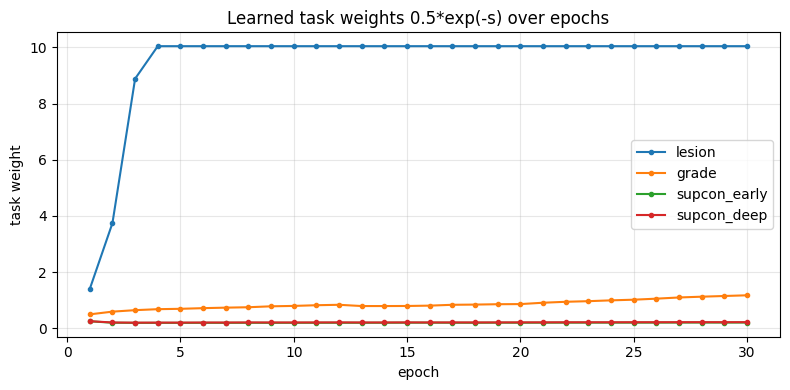
\includegraphics[width=\columnwidth]{exp7-weights.png}}
\caption{Learned task weights $w_i=\tfrac12 e^{-s_i}$ over $30$ epochs
(Eq.~\eqref{eq:uw}). The lesion weight saturates at its clamp ceiling
($\approx10.0$) by epoch~$4$ and stays pinned, while the grade weight rises
gradually to $\approx1.2$ and the two contrastive weights remain near $0.2$. The
saturation is the core diagnostic: the uncertainty mechanism strongly---but not
adaptively---prioritised the lesion task.}
\label{fig:exp7_weights}
\end{figure}

\begin{figure}[!t]
\centerline{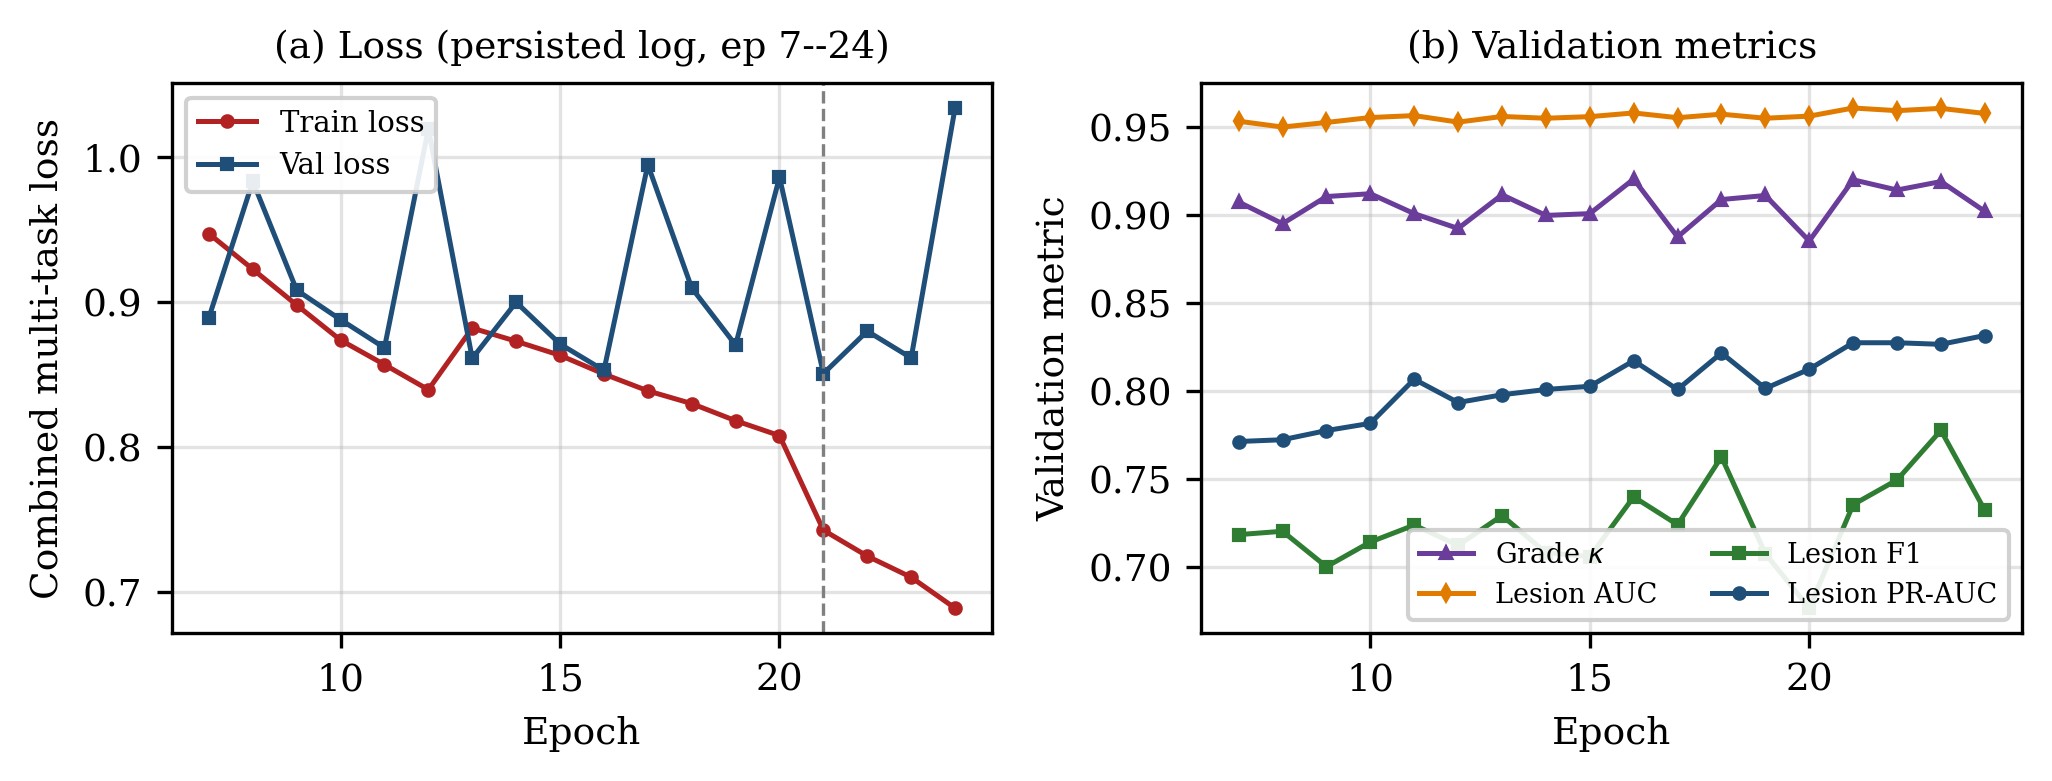
\includegraphics[width=\columnwidth]{exp7-training-curves.png}}
\caption{Experiment~VII training dynamics (persisted log, epochs $7$--$24$).
(a)~Training loss falls steadily while validation loss oscillates around the
epoch-$21$ minimum (dashed line). (b)~Lesion macro-AUROC ($\approx0.96$), grade
$\kappa$ ($\approx0.91$), and lesion PR-AUC rise gently; PR-AUC climbs from $0.77$
to $0.83$, indicating improving ranking of the rare lesions.}
\label{fig:exp7_curves}
\end{figure}

\subsection{Analysis}
The clamp saturation means Experiment~VII is best read as an empirical upper bound
on what a heavily lesion-weighted version of the Experiment-VI network achieves:
the strongest lesion F1/AUROC/PR-AUC and rare-class recall in the study. The grade
weight's smooth rise shows the uncertainty parameters \emph{did} adapt for the
well-behaved grade and contrastive tasks; only the lesion task hit the numerical
boundary.

\subsection{Discussion}
The result is a genuine improvement in rare-lesion detection but is only partly
attributable to ``learned'' weighting---the lesion component effectively reverted to
a large fixed weight. A wider clamp, a smaller log-variance learning rate, or the
analytic softmax-normalised variant would let the lesion weight settle rather than
rail, and would make the adaptivity claim cleaner. The two persisted checkpoints
(\texttt{best\_model (1).pth}, \texttt{checkpoint (2).pth}) preserve this state for
reuse.

\subsection{Limitations}
The lesion log-variance is pinned at the clamp for the entire run, so the
weighting is not fully adaptive. The persisted CSV covers epochs $7$--$24$ while the
run reached $30$; peak values are drawn from the union of the CSV and the checkpoint
log. The split is random and unstratified, validation doubles as evaluation, and
although a seed is fixed the run is single-seed. The run used the four-task
(``weight all tasks'') configuration rather than the grade-plus-lesion-only variant.

\subsection{Conclusion}
Homoscedastic-uncertainty weighting applied to the contrastive UWF network yields
the study's best rare-lesion detection (lesion F1 up to $0.778$, AUROC up to
$0.961$; rare recall NV/VH/RD $=0.89/0.95/0.96$), but the lesion weight saturated at
its clamp, so the gain reflects strong fixed prioritisation more than fully learned
balancing.

% ===========================================================================
\section{Experiment VIII: Recall-Driven Curriculum Resampling (UWF)}
\label{sec:exp8}

\subsection{Objective}
Experiment~VIII addresses rare-lesion sensitivity from the \emph{data-sampling}
side. Holding the Experiment-VI network and loss fixed, it makes the training
sampler the only independent variable: a recall-driven curriculum resampler
(RDCR) that oversamples classes the model is currently missing.

\subsection{Motivation}
Loss re-weighting (Experiments~IV--VII) changes how much each example counts;
resampling changes which examples enter the batch. A static rarity-based sampler
must guess a fixed oversampling ratio in advance. RDCR instead adapts the ratio
online from validation recall, so effort tracks the classes that are actually being
missed, and it fixes a standing weakness of the earlier experiments by using a
\emph{stratified} split.

\subsection{Methodology}
Twelve rebalancing channels (five grades, seven lesions) each carry an importance
$I_k = \pi_k^{a}\,(D_k+\epsilon)^{b}$, where $\pi_k$ is a static effective-number
rarity prior~\cite{effnum} and $D_k$ is an exponential-moving-average of the class
\emph{deficit} $1-\mathrm{recall}_k$ measured on validation each epoch. A sample's
weight collapses its channel importances by a max reduction (avoiding
double-counting co-occurring PDR lesions). A curriculum temperature $\tau(\text{epoch})$
holds sampling uniform for a warmup ($5$ epochs) then ramps the importances in over
$15$ epochs, and the final per-sample weights are clamped to a maximum ratio of
$20{:}1$ to limit rare-image repetition. The sampler feeds a
\texttt{WeightedRandomSampler}; the loss (asymmetric focal $+$ CE $+$ two SupCon
terms) is unchanged. A CPU unit test asserts the sampler up-weights a deliberately
starved rare class.

\subsection{Experimental Setup}
Implemented in PyTorch across two CUDA GPUs (\texttt{DataParallel}) with AMP, a fixed
seed, and deterministic cuDNN. The sampler's deficit state is checkpointed so a
resumed run continues the controller and curriculum.

\subsection{Dataset}
The UWF subset is split 80/20 with seed $42$, \emph{stratified on the rare-lesion
indicator}---the only experiment here to do so---giving $8{,}323$ training and
$2{,}081$ validation images. Because the validation split differs from the random
split of Experiments~III--VII, its metrics are not directly comparable to them.

\subsection{Preprocessing}
Identical to Experiment~VI: resize to $512\times512$, elliptical
\texttt{apply\_uwf\_mask} (\texttt{tightness}~$=0.98$), ImageNet normalisation, and
flip/colour-jitter/rotation ($\pm10^{\circ}$) training augmentation---augmentation
is also the primary defence against oversampling overfitting, so repeatedly drawn
rare images look different on each draw.

\subsection{Architecture}
Experiment~VI's \texttt{UWF\_SupConDRNet} (ResNet-50 + FPN + two SupCon heads),
unchanged, so that any change in behaviour is attributable to the sampler alone.

\subsection{Training Procedure}
Training was scheduled for $60$ epochs with early stopping (patience $10$) on
validation loss and \texttt{ReduceLROnPlateau} (factor $0.5$, patience $3$),
gradient clipping at $2.0$. Each epoch rebuilds the sampler from the previous
epoch's recall deficit and the current curriculum $\tau$; the warmup ends at
epoch~$5$ and the ramp completes by epoch~$20$. The persisted metrics log covers
$18$ epochs.

\subsection{Hyperparameters}
Table~\ref{tab:exp8_hyper} lists the configuration.

\begin{table}[!t]
\caption{Experiment~VIII --- Training and Sampler Configuration}
\label{tab:exp8_hyper}
\centering
\setlength{\tabcolsep}{5pt}
\begin{tabular}{|l|l|}
\hline
\textbf{Setting} & \textbf{Value} \\
\hline
Backbone / loss & \texttt{UWF\_SupConDRNet} / folder-VI combined \\
Compute & $2\times$ GPU (\texttt{DataParallel}), AMP \\
Input resolution & $512\times512$ \\
Split & 80/20, seed $42$, \textbf{stratified} on rare flag \\
Optimiser & AdamW, lr $1\times10^{-4}$, wd $1\times10^{-4}$ \\
Batch size & $8$ \\
Gradient clipping & max-norm $2.0$ \\
Rarity prior & Effective-number~\cite{effnum}, $\beta{=}0.999$, $a{=}0.5$ \\
Deficit EMA & $m{=}0.7$, exponent $b{=}1$, floor $\epsilon{=}10^{-3}$ \\
Curriculum & warmup $5$ ep, ramp $15$ ep ($\tau{:}0{\to}1$) \\
Weight-ratio clamp & $\rho_{\max}=20$ \\
Epochs (planned / logged) & $60$ / $18$ \\
\hline
\end{tabular}
\end{table}

\subsection{Evaluation Metrics}
Quadratic-weighted Cohen's~$\kappa$ (grade), lesion macro-F1 and macro-AUROC, and
per-rare-class recall (NV/VH/RD), logged each epoch. Grade accuracy is not recorded
in the persisted log; $\kappa$ is the grade headline.

\subsection{Results}
As the curriculum engages after the epoch-$5$ warmup, grade $\kappa$ and lesion
AUROC rise together (Fig.~\ref{fig:exp8_curves}a): $\kappa$ climbs from $\approx0.87$
to a peak of $\textbf{0.9234}$ (epoch~$14$), lesion AUROC to $0.9455$ (epoch~$18$),
and lesion macro-F1 to $0.7088$ (epoch~$17$). The rare-class recalls
(Fig.~\ref{fig:exp8_curves}b) are the headline: RD recall reaches $1.0$ at
epochs~$7$--$8$ as the ramp begins, and NV/VH range over roughly $0.83$--$0.96$,
though all three are volatile---expected given only $\sim45$ RD positives in the
validation split. The lowest validation loss is at epoch~$12$ ($2.369$).
Table~\ref{tab:exp8_res} summarises the values.

\begin{table}[!t]
\caption{Experiment~VIII --- Validation Results (Stratified Split)}
\label{tab:exp8_res}
\centering
\setlength{\tabcolsep}{5pt}
\begin{tabular}{|l|c|c|}
\hline
\textbf{Metric} & \textbf{Epoch 12 (selected)} & \textbf{Best (epoch)} \\
\hline
Grade $\kappa$ (quad.) & $0.9144$ & $0.9234$ ($14$) \\
Lesion macro-AUROC & $0.9423$ & $0.9455$ ($18$) \\
Lesion macro-F1 & $0.7011$ & $0.7088$ ($17$) \\
RD recall & $0.889$ & $1.000$ ($7$--$8$) \\
NV recall & $0.879$ & $0.957$ ($1$) \\
VH recall & $0.914$ & $0.951$ ($1$) \\
\hline
\multicolumn{3}{|l|}{Stratified split---not directly comparable to Exp.~III--VII.} \\
\hline
\end{tabular}
\end{table}

\begin{figure}[!t]
\centerline{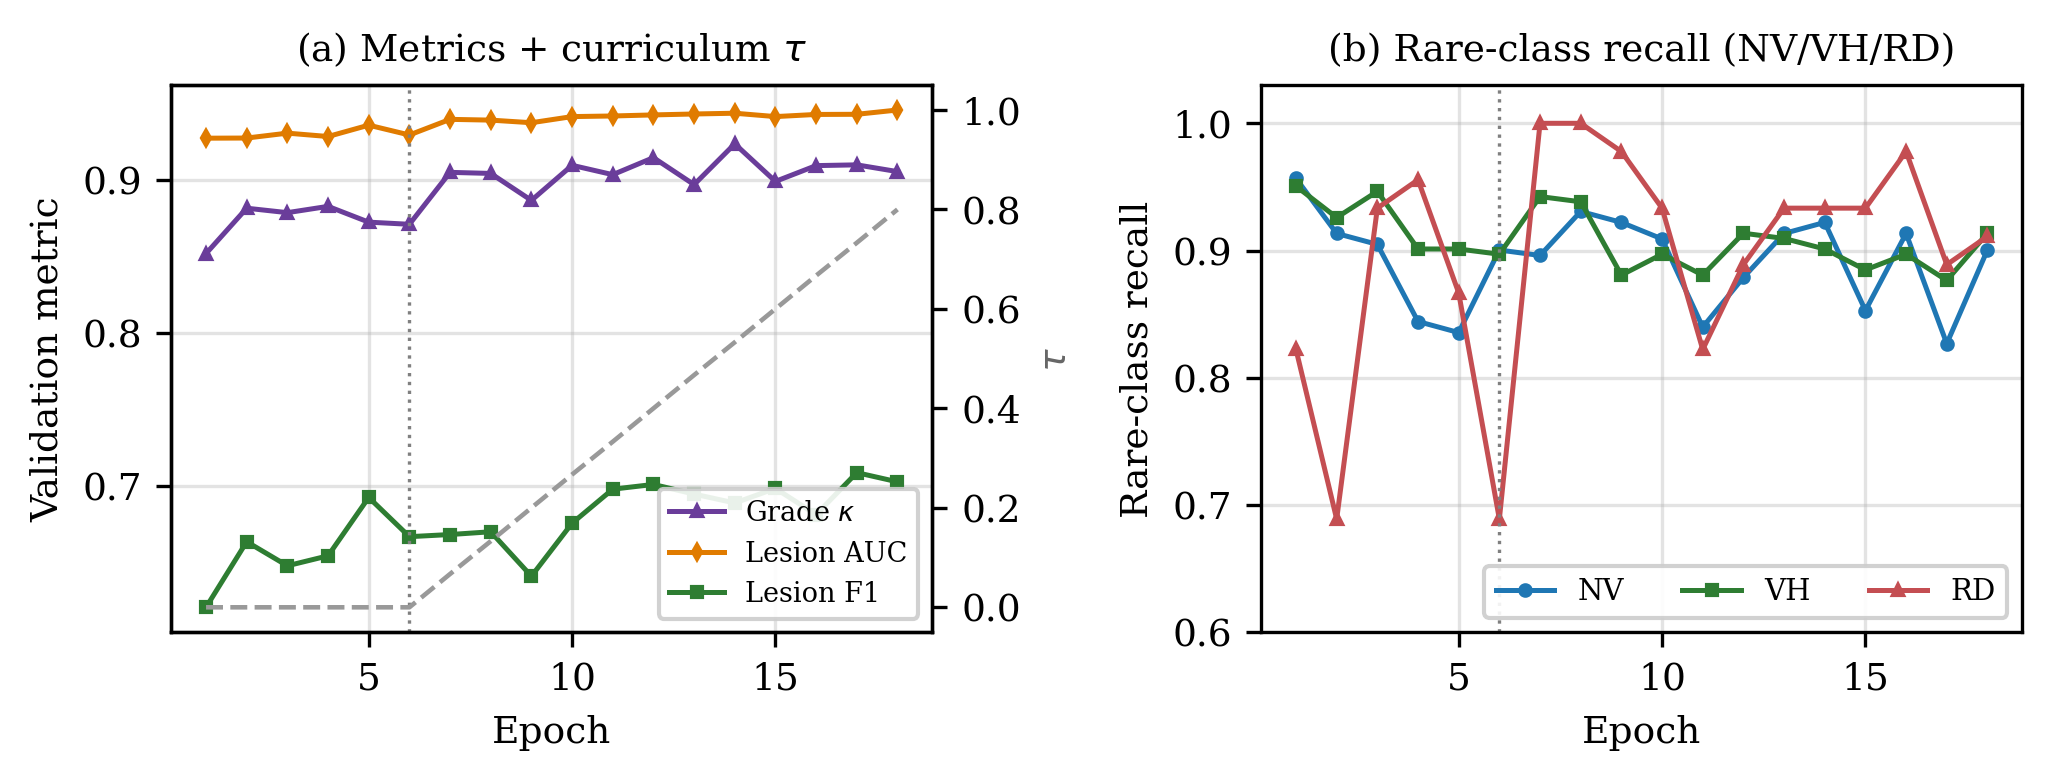
\includegraphics[width=\columnwidth]{exp8-training-curves.png}}
\caption{Experiment~VIII dynamics over $18$ logged epochs. (a)~Grade $\kappa$,
lesion AUROC, and lesion F1 rise as the curriculum $\tau$ (dashed, right axis) ramps
in after the epoch-$5$ warmup (dotted line). (b)~Per-rare-class recall: RD reaches
$1.0$ once the ramp engages; NV/VH remain high but volatile, reflecting the very
small number of rare positives in the validation split.}
\label{fig:exp8_curves}
\end{figure}

\subsection{Analysis}
The curriculum has the intended effect: rare-class recall improves as $\tau$ ramps,
and grade $\kappa$ reaches its peak ($0.9234$) in the same window, so rebalancing
the sampler did not harm grading. The volatility of RD recall is a direct
consequence of the tiny rare-positive count and is why per-epoch recall, not a
single final number, is the honest way to report it.

\subsection{Discussion}
Because the backbone and loss are frozen, the gains isolate the sampler's
contribution. On its own (stratified) validation set RDCR matches the mature
folder-VI baseline on grade $\kappa$ ($\approx0.92$) and lesion AUROC
($\approx0.945$) while pushing rare recall high---but it does not clearly beat the
baseline, and the comparison is confounded by the different split. The stratified
split is itself the more rigorous protocol and is the main methodological
contribution here.

\subsection{Limitations}
Only $18$ of $60$ planned epochs are logged, and no checkpoint was preserved on
disk. The run is single-seed. Grade accuracy is absent from the log. Most
importantly, the stratified split makes the numbers non-comparable to the other
experiments, so ``matched baseline'' is a qualitative statement, not a controlled
head-to-head; a like-for-like comparison would require rerunning the baseline on the
same stratified split with multiple seeds.

\subsection{Conclusion}
Recall-driven curriculum resampling, with the network and loss held fixed, lifts
rare-class recall (RD to $1.0$, NV/VH $\approx0.9$) and reaches grade $\kappa=0.923$
and lesion AUROC $0.946$ on a stratified split, demonstrating adaptive sampling as a
viable, backbone-agnostic route to rare-lesion sensitivity, pending a multi-seed,
same-split comparison.

% ===========================================================================
\section{Experiment IX: Shared vs.\ Separate Lesion Heads (UWF)}
\label{sec:exp9}

\subsection{Objective}
Experiment~IX is a controlled architectural ablation: does giving the rare
PDR lesions their own \emph{dedicated} classification head improve their detection,
once the effect is separated from the effect of simply adding head capacity? It
holds the entire trunk and loss fixed and varies only the lesion head, on a proper
held-out test split.

\subsection{Motivation}
In a single shared lesion head, the gradient from the $6$--$30\times$ more frequent
common lesions can dominate the parameters that also serve the rare lesions. A
natural hypothesis is that a \emph{separate} rare-lesion head, decoupled from the
common lesions, would be freed from this domination and detect NV/VH/RD better. But
a separate head also adds parameters, so a fair test needs a capacity-matched
control that keeps the head shared---otherwise any gain could be mere capacity.

\subsection{Methodology}
Three head variants share an identical trunk and differ only in
\texttt{classifier\_lesions}: \textbf{A (shared)}, a single \texttt{Linear(512,7)}
($3{,}591$ head params); \textbf{A$'$ (shared-MLP)}, a two-layer MLP over all seven
lesions ($66{,}567$ params); and \textbf{B (separate)}, a linear head for the four
common lesions plus a dedicated MLP head for the three rare lesions ($68{,}103$
params). A$'$ and B are capacity-matched, so the contrast $\text{B}-\text{A}'$
isolates \emph{separation} while $\text{A}'-\text{A}$ isolates \emph{capacity}. The
split head concatenates \texttt{[common\,|\,rare]} logits, which is exactly the
canonical lesion order, so the loss and metrics are variant-agnostic. Six CPU
unit tests verify the design: identical trunk size across variants
($26{,}921{,}797$ params), exact head-parameter counts, rare-logit gradients
touching only the rare sub-head, loss reduction-consistency (split $=$ shared), and
that per-lesion threshold tuning beats a fixed $0.5$ on rare recall.

\subsection{Experimental Setup}
Implemented in PyTorch across two CUDA GPUs (\texttt{DataParallel}) with AMP, fixed
seeds, and deterministic cuDNN. Model selection uses a composite score
($0.5\times$rare recall $+\,0.5\times$macro-F1) on validation, and per-lesion
decision thresholds are tuned on validation before the test evaluation. Unusually
for this study, evaluation uses a genuine held-out test split, not the validation
set.

\subsection{Dataset}
The UWF subset is divided into a \emph{three-way} $70/15/15$ train/validation/test
split, stratified on the rare-lesion indicator with seed $42$: $7{,}282$ training,
$1{,}561$ validation, and $1{,}561$ test images, with a matched rare-positive
fraction of $\approx0.149$ in every partition. All reported numbers are on the
held-out test split.

\subsection{Preprocessing}
The standard UWF pipeline: resize to $512\times512$, elliptical
\texttt{apply\_uwf\_mask} (\texttt{tightness}~$=0.98$), ImageNet normalisation, and
flip/colour-jitter/rotation training augmentation.

\subsection{Architecture}
\texttt{MultiHeadDRNet} is the folder-VI \texttt{UWF\_SupConDRNet} trunk (ResNet-50 +
FPN + two SupCon projection heads + a grade head), byte-identical across variants,
with only the lesion head swapped. The shared trunk, grade head, and contrastive
heads are therefore controlled, so any measured difference is attributable to the
lesion head alone.

\subsection{Training Procedure}
The combined loss is the folder-VI objective (asymmetric focal on lesions, grade
cross-entropy with label smoothing $0.05$, and two SupCon terms). The reported run
is a single-seed \texttt{QUICK\_PASS} of $20$ epochs per variant (the full protocol
is $60$ epochs $\times 3$ seeds, designed and resumable but not run here). Because
the run was assembled across resumable sessions, the shared and shared-MLP variants
were continued from earlier checkpoints while the separate variant trained afresh
and early-stopped at epoch~$14$; the training budgets are therefore not perfectly
matched, so the comparison is preliminary.

\subsection{Hyperparameters}
Table~\ref{tab:exp9_hyper} lists the configuration.

\begin{table}[!t]
\caption{Experiment~IX --- Training Configuration}
\label{tab:exp9_hyper}
\centering
\setlength{\tabcolsep}{5pt}
\begin{tabular}{|l|l|}
\hline
\textbf{Setting} & \textbf{Value} \\
\hline
Trunk & \texttt{UWF\_SupConDRNet} (ResNet-50 + FPN) \\
Variable component & Lesion head only (A / A$'$ / B) \\
Head params (A/A$'$/B) & $3{,}591$ / $66{,}567$ / $68{,}103$ \\
Compute & $2\times$ GPU (\texttt{DataParallel}), AMP \\
Input resolution & $512\times512$ \\
Split & 70/15/15, seed $42$, stratified (held-out test) \\
Optimiser & AdamW, lr $1\times10^{-4}$, wd $1\times10^{-4}$ \\
Batch size & $16$ \\
Loss & Asym.\ focal $+$ CE (LS $0.05$) $+ 0.5$ SupCon$\times2$ \\
Selection & Composite ($0.5$ rare recall $+\,0.5$ macro-F1) \\
Thresholds & Per-lesion, tuned on validation \\
Epochs (this pass / full) & $20\times1$ seed / $60\times3$ seeds \\
\hline
\end{tabular}
\end{table}

\subsection{Evaluation Metrics}
On the held-out test split: lesion macro-F1, mean rare-class (NV/VH/RD) recall, and
grade quadratic-weighted Cohen's~$\kappa$, computed with the tuned per-lesion
thresholds.

\subsection{Results}
Table~\ref{tab:exp9_res} and Fig.~\ref{fig:exp9_heads} give the held-out test
results. The dedicated rare head (B) does \emph{not} help: its mean rare-class
recall ($0.816$) is the lowest of the three and well below the capacity-matched
shared-MLP control (A$'$, $0.890$) and even the minimal shared linear head
(A, $0.884$). Reading the two contrasts, capacity alone ($\text{A}'-\text{A}$) moves
rare recall by only $+0.006$ and slightly lowers macro-F1 ($0.698$ vs.\ $0.707$),
while separation ($\text{B}-\text{A}'$) \emph{reduces} rare recall by $0.074$. The
plain shared head attains the best lesion macro-F1 ($0.707$) and a grade $\kappa$
($0.914$) on par with A$'$ ($0.915$).

\begin{table}[!t]
\caption{Experiment~IX --- Held-Out Test Results (Single-Seed, 20-Epoch Pass)}
\label{tab:exp9_res}
\centering
\setlength{\tabcolsep}{4pt}
\begin{tabular}{|l|c|c|c|c|}
\hline
\textbf{Variant} & \textbf{Head params} & \textbf{Rare rec.} &
\textbf{Macro-F1} & \textbf{$\kappa$} \\
\hline
A\phantom{$'$} (shared linear) & $3{,}591$ & $0.884$ & $\mathbf{0.707}$ & $0.914$ \\
A$'$ (shared MLP) & $66{,}567$ & $\mathbf{0.890}$ & $0.698$ & $\mathbf{0.915}$ \\
B\phantom{$'$} (separate) & $68{,}103$ & $0.816$ & $0.689$ & $0.886$ \\
\hline
\multicolumn{5}{|l|}{Rare rec.\ = mean recall over NV/VH/RD. Best per column in
\textbf{bold}.} \\
\hline
\end{tabular}
\end{table}

\begin{figure}[!t]
\centerline{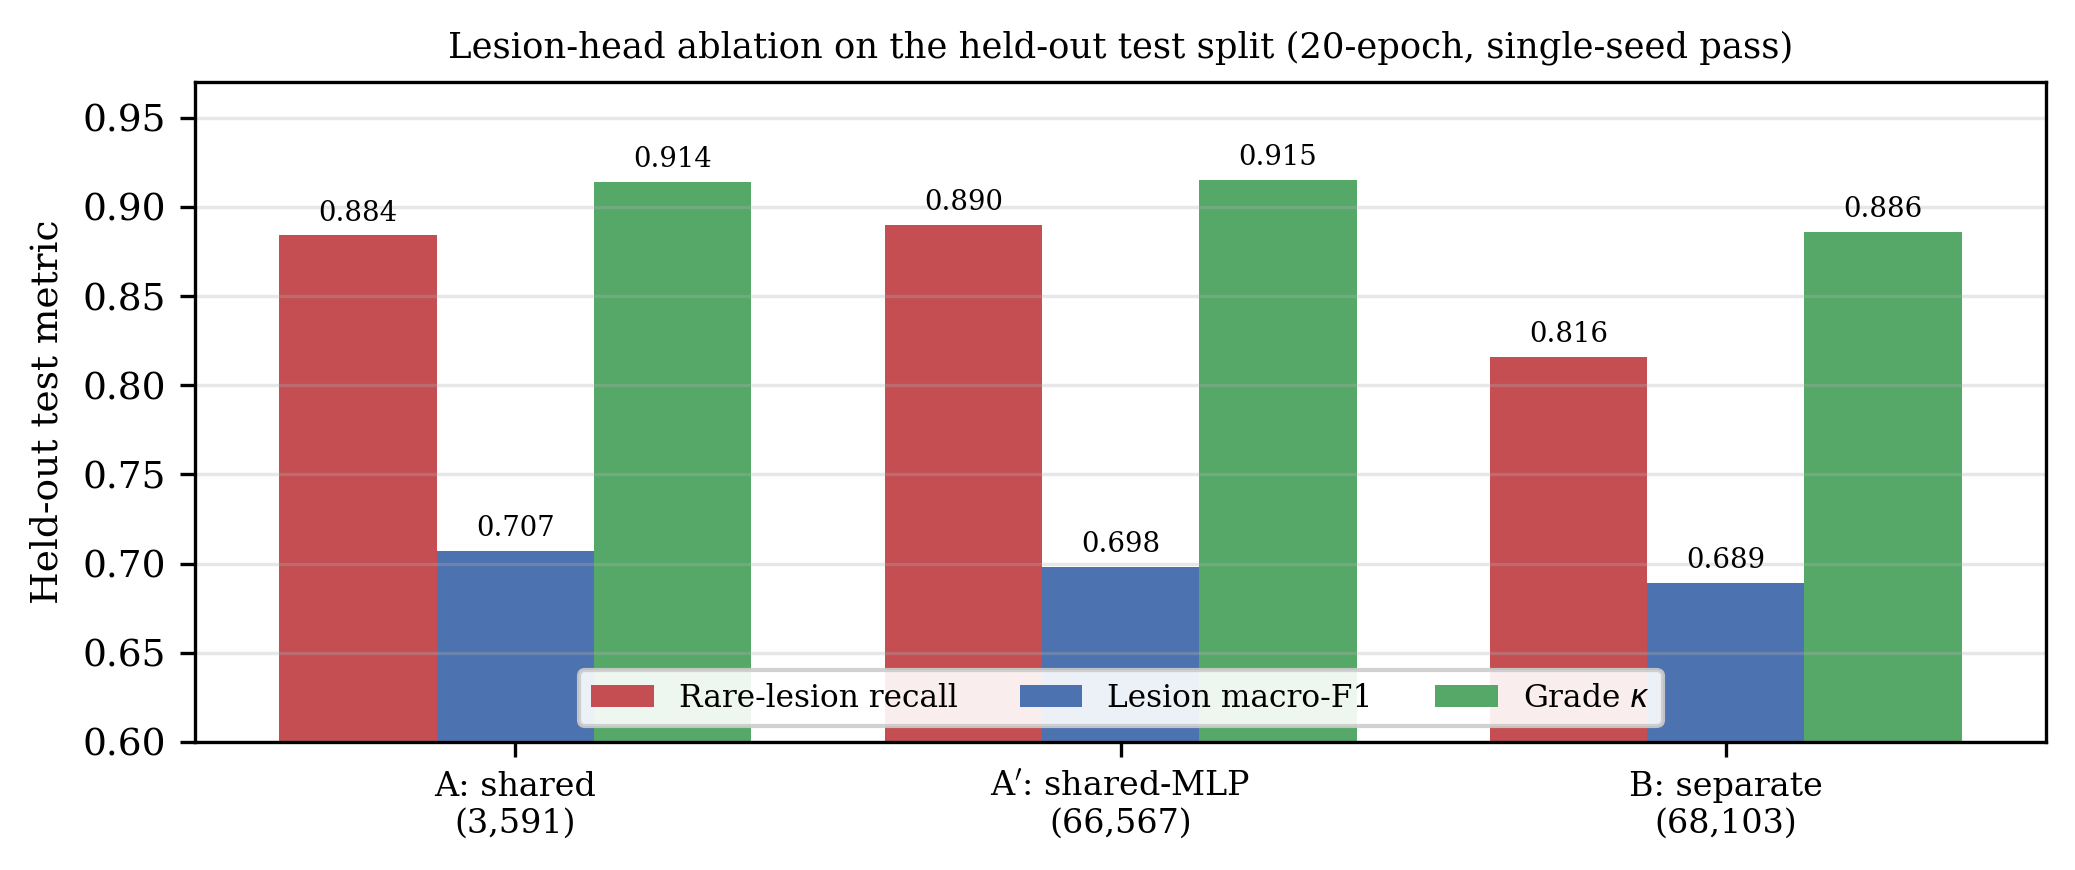
\includegraphics[width=\columnwidth]{exp9-heads.png}}
\caption{Held-out test metrics for the three capacity-controlled lesion heads.
Adding head capacity (A$\rightarrow$A$'$) barely changes any metric, and separating
the rare head (A$'$$\rightarrow$B) \emph{lowers} rare-lesion recall from $0.890$ to
$0.816$. The simple shared linear head (A) is the strongest on macro-F1 and
competitive on rare recall and $\kappa$.}
\label{fig:exp9_heads}
\end{figure}

\subsection{Analysis}
The controlled design turns a plausible intuition into a testable claim and refutes
it: on this preliminary single-seed pass, neither extra head capacity nor an
explicit rare/common split improves held-out rare-lesion detection over a plain
\texttt{Linear(512,7)} head. The likely reason is that the rare-lesion signal is
limited by the trunk features and the rare-positive count, not by head-level
gradient competition, so a bigger or decoupled head mostly adds variance (and B's
fresh, shorter training compounds this).

\subsection{Discussion}
The value here is methodological: a capacity-matched control (A$'$) and a genuine
held-out test split make the negative result trustworthy, and the unit tests
guarantee the variants differ only where intended. It suggests that, for this
backbone, rare-lesion gains are more likely to come from the trunk, the loss, or
the data (Experiments~IV--VIII) than from the head topology. The tuned-threshold
step is a cheap, orthogonal lever that helped rare recall in the unit test and is
retained for all variants.

\subsection{Limitations}
This is a single-seed, $20$-epoch preliminary pass, not the pre-registered
$60$-epoch $\times 3$-seed protocol, and the variants were trained across sessions
with unequal effective budgets (B trained fresh and early-stopped while A/A$'$
resumed), so the ranking may shift under matched, multi-seed training with a
significance test. No checkpoints were retained locally.

\subsection{Conclusion}
A controlled, capacity-matched ablation on a held-out test split finds that a
dedicated rare-lesion head does not improve---and in this pass slightly harms---
rare-lesion detection relative to a shared head ($0.816$ vs.\ $0.890$ mean rare
recall), indicating that head topology is not the bottleneck for rare-lesion
sensitivity in this pipeline.

% ===========================================================================
\section{Experiment X: Synthetic Minority Generation (UWF)}
\label{sec:exp10}

\subsection{Objective}
Experiment~X generates \emph{new} synthetic rare-lesion images with a conditional
diffusion model, as an alternative to oversampling the same scarce positives, and
runs the decisive test: does adding those images to training raise rare-class recall
on a $100\%$-real held-out test set, versus a real-only baseline and versus classic
oversampling? A full-scale generator was trained and the downstream study was run to
completion; the result is a clean negative verdict.

\subsection{Motivation}
With only $238$ retinal-detachment positives ($2.3\%$ of UWF), oversampling can
only duplicate the same few images, so the classifier memorises them rather than
learning what the lesion looks like. A generative model that synthesises plausible
new rare-lesion retinas could add genuine variety, potentially improving
rare-class recall beyond what duplication achieves.

\subsection{Methodology}
The runnable proof-of-concept is a compact, from-scratch \emph{conditional
pixel-space DDPM}~\cite{ddpm}. The forward process adds Gaussian noise to a real
masked retina over $T{=}200$ steps; a small U-Net $\epsilon_\theta(x_t,t,y)$ is
trained to predict that noise by the DDPM simple objective
$\mathbb{E}\lVert\epsilon-\epsilon_\theta\rVert^2$, conditioned on a rare-flag $y$.
Classifier-free guidance~\cite{cfg} is enabled by dropping the condition with
probability $0.10$ during training and, at sampling, extrapolating
$\hat\epsilon = \epsilon_\theta(x_t,\varnothing) + w\,(\epsilon_\theta(x_t,y) -
\epsilon_\theta(x_t,\varnothing))$ with guidance scale $w{=}3$
(Fig.~\ref{fig:exp10_method}). The documented production generator is a
LoRA-fine-tuned latent-diffusion model~\cite{ldm} at $256\times256$; the compact
pixel-space slice shares the same objective at a size that trains within a session.
\begin{figure}[!t]
\centerline{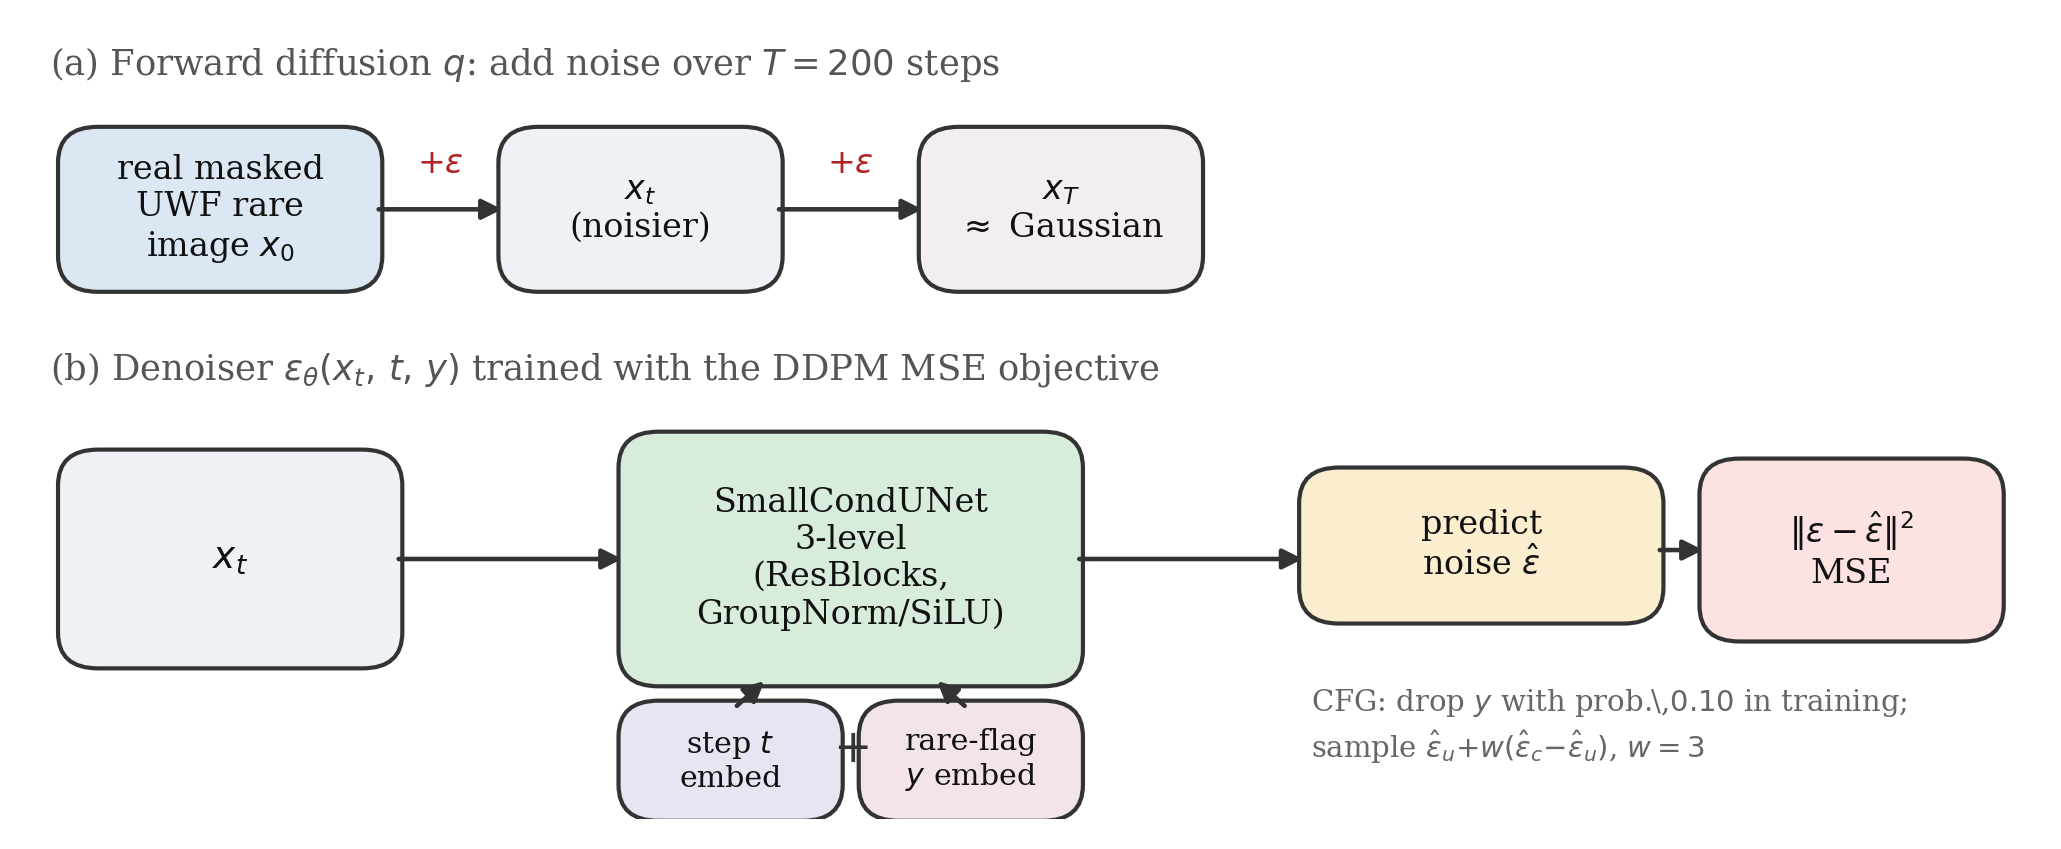
\includegraphics[width=\columnwidth]{exp10-method.png}}
\caption{Conditional-DDPM pipeline (method schematic drawn from the notebook code,
not an experimental result). (a)~The forward process noises a real masked rare-lesion
retina over $T{=}200$ steps. (b)~\texttt{SmallCondUNet} $\epsilon_\theta(x_t,t,y)$
predicts the added noise under an MSE objective, conditioned on the timestep and
rare-flag embeddings; classifier-free guidance drops the condition with probability
$0.10$ in training and extrapolates with scale $w{=}3$ at sampling.}
\label{fig:exp10_method}
\end{figure}

\subsection{Experimental Setup}
Implemented in PyTorch with AMP and optional multi-GPU, and structured with
checkpoint/resume and dataset backup for multi-session training. Optional generative
libraries are guarded so the pipeline runs on the pre-installed stack alone.

\subsection{Dataset}
The generator is trained on the UWF rare-positive images (any of NV/VH/RD present;
$1{,}555$ images, with RD only $238$). Provenance is tracked so synthetic images are
always labelled synthetic and never stored as real patient data (MMRDR is CC0).

\subsection{Preprocessing}
Each retina is resized to $512$, masked with the elliptical
\texttt{apply\_uwf\_mask}, downscaled to the generator resolution ($64\times64$ in
the slice), and normalised to $[-1,1]$; a one-time cache of masked tensors speeds
up epochs.

\subsection{Architecture}
\texttt{SmallCondUNet} is a three-level conditional U-Net of residual blocks
(GroupNorm/SiLU). Conditioning enters by adding a sinusoidal timestep embedding and
a learned rare-flag class embedding; a learned null token supports classifier-free
guidance.

\subsection{Training Procedure}
AdamW (lr $2\times10^{-4}$) with a cosine schedule, AMP, gradient clipping at $1.0$,
and rolling/best checkpointing to a Kaggle dataset for multi-session resume. The
reported run used \texttt{MODE=full} on two T4 GPUs over the real UWF rare-positive
set ($650$ steps/epoch, $\approx66$\,s/epoch), reaching epoch~$41$ of a planned
$50$; the best epoch-average loss was at epoch~$39$.

\subsection{Hyperparameters}
Table~\ref{tab:exp10_hyper} lists the slice configuration.

\begin{table}[!t]
\caption{Experiment~X --- Proof-of-Concept Generator Configuration}
\label{tab:exp10_hyper}
\centering
\setlength{\tabcolsep}{5pt}
\begin{tabular}{|l|l|}
\hline
\textbf{Setting} & \textbf{Value} \\
\hline
Generator & Conditional pixel-space DDPM (\texttt{SmallCondUNet}) \\
Resolution & $64\times64$ (production target $256$) \\
Diffusion steps $T$ & $200$ (production $\sim1000$) \\
Objective & DDPM $\epsilon$-prediction MSE~\cite{ddpm} \\
Guidance & Classifier-free~\cite{cfg}, drop $0.10$, $w{=}3$ \\
Optimiser & AdamW, lr $2\times10^{-4}$, cosine \\
Batch size & $16$ \\
Gradient clipping & max-norm $1.0$ \\
Generator params & $3.86$\,M (\texttt{SmallCondUNet}) \\
Run & \texttt{full}, $2\times$T4, ep~$41/50$ ($\approx26.6$k steps) \\
Best epoch-avg loss & $0.0161$ (epoch $39$) \\
Production generator & LoRA latent diffusion~\cite{ldm} (documented) \\
\hline
\end{tabular}
\end{table}

\subsection{Evaluation Metrics}
Generative quality is checked with FID~\cite{fid} and unbiased KID, computed between
real and synthetic rare-lesion images at both the generator's native $64\times64$ and
the study's $256\times256$ resolution, each against a real-vs-real floor. The
decisive metric, however, is \emph{downstream utility}: per-rare-class recall on a
fixed, $100\%$-real held-out test set when the folder-VI classifier
(\texttt{UWF\_SupConDRNet}) is trained under three regimes---real only,
real$+$oversampling, and real$+$synthetic---on one frozen stratified 70/15/15 split
(train $7{,}282$ / val $1{,}561$ / test $1{,}561$, signature \texttt{da1ec8e21f22}).
The validation and test sets are $100\%$ real and identical across regimes; per-lesion
thresholds are fitted on validation only. Grade quadratic $\kappa$ and common-lesion
macro-F1 act as collateral-damage guardrails.

\subsection{Results}
\emph{Generator.} The DDPM $\epsilon$-prediction MSE fell from $0.081$ at epoch~$1$ to
a best epoch-average of $\mathbf{0.0161}$ at epoch~$39$ (Fig.~\ref{fig:exp10_loss}),
converging stably; classifier-free sampling produces diverse conditional images (mean
pairwise sample distance $29.9$, i.e.\ no mode collapse).

\emph{Generation quality is poor at this scale.} Synthetic-vs-real FID is $200.0$ at
$64$px and $246.9$ at $256$px, against real-vs-real floors of only $26.8$ and $29.2$
(KID $0.256$ and $0.326$). The synthetic images are therefore far from the real
distribution. Fig.~\ref{fig:exp10_samples} shows why: the samples reproduce the
elliptical field of view and the green/orange UWF colouration but contain no
recognisable vasculature or lesion structure.

\emph{The downstream verdict is negative.} Table~\ref{tab:exp10_res} and
Fig.~\ref{fig:exp10_verdict} give the held-out-test results. The real-only baseline
is already strong on rare-class recall ($0.878$); adding synthetic images
\emph{lowers} it to $0.833$, and classic oversampling lowers it further to $0.807$.
Synthetic augmentation also slightly regressed both guardrails (grade $\kappa$
$0.892$ vs.\ $0.902$; common-lesion F1 $0.716$ vs.\ $0.723$). By the pre-registered
rule---beat \emph{both} real and oversampling on mean rare recall without regressing
the guardrails---the verdict is \textbf{False}: at proof-of-concept resolution,
generated data does not improve rare-lesion detection. The damage is concentrated in
retinal detachment, the rarest class ($31$ test positives), whose recall falls from
$0.839$ (real) to $0.710$ (synthetic).

\begin{table}[!t]
\caption{Experiment~X --- Downstream Verdict on the $100\%$-Real Test Set (seed $42$)}
\label{tab:exp10_res}
\centering
\setlength{\tabcolsep}{4pt}
\begin{tabular}{|l|c|c|c|}
\hline
\textbf{Metric (real test)} & \textbf{real} & \textbf{+oversample} & \textbf{+synthetic} \\
\hline
Mean rare recall & $\mathbf{0.878}$ & $0.807$ & $0.833$ \\
\quad NV recall & $0.894$ & $0.806$ & $0.888$ \\
\quad VH recall & $0.900$ & $0.842$ & $0.900$ \\
\quad RD recall & $\mathbf{0.839}$ & $0.774$ & $0.710$ \\
Rare macro-F1 & $0.687$ & $\mathbf{0.714}$ & $0.656$ \\
Rare macro PR-AUC & $0.653$ & $\mathbf{0.797}$ & $0.665$ \\
Grade $\kappa$ (guardrail) & $\mathbf{0.902}$ & $0.880$ & $0.892$ \\
Common-lesion F1 (guardrail) & $\mathbf{0.723}$ & $0.717$ & $0.716$ \\
\hline
\multicolumn{4}{|l|}{\footnotesize Best per row in \textbf{bold}. Verdict rule: synthetic
must beat \emph{both}} \\
\multicolumn{4}{|l|}{\footnotesize other columns on mean rare recall without regressing the
guardrails $\rightarrow$ \textbf{not met}.} \\
\hline
\end{tabular}
\end{table}

\begin{figure}[!t]
\centerline{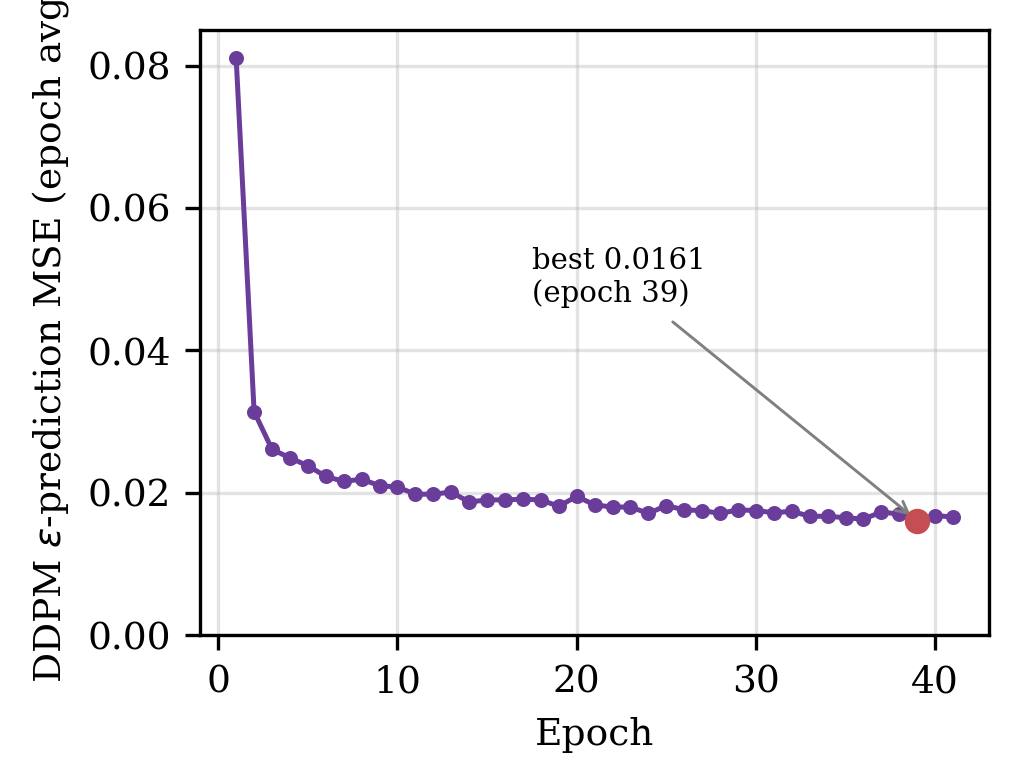
\includegraphics[width=\columnwidth]{exp10-loss.png}}
\caption{Experiment~X generator training. The DDPM noise-prediction MSE (epoch
average) decreases from $0.081$ to a best of $0.0161$ at epoch~$39$ over the
$41$-epoch \texttt{full} run on the real UWF rare-positive set, indicating stable
convergence of the conditional diffusion model.}
\label{fig:exp10_loss}
\end{figure}

\begin{figure}[!t]
\centerline{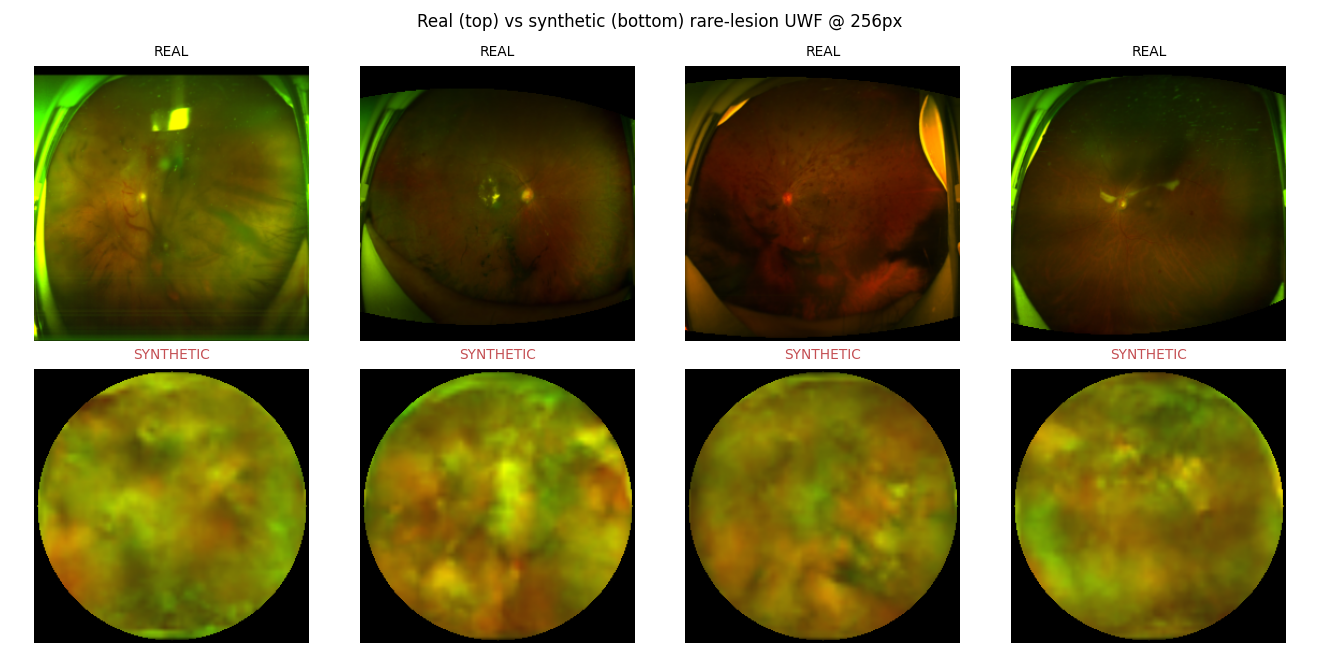
\includegraphics[width=\columnwidth]{exp10-realsynth256.png}}
\caption{Real UWF retinas (top) versus rare-conditioned synthetic samples
(bottom, guidance $w{=}3$), shown at the study's $256\times256$. The generator
captures the field of view and colouration but no vasculature or lesion structure,
consistent with the very high synthetic-vs-real FID ($246.9$ vs.\ a $29.2$ floor).
Synthetic images are always labelled synthetic and never treated as real patient
data.}
\label{fig:exp10_samples}
\end{figure}

\begin{figure}[!t]
\centerline{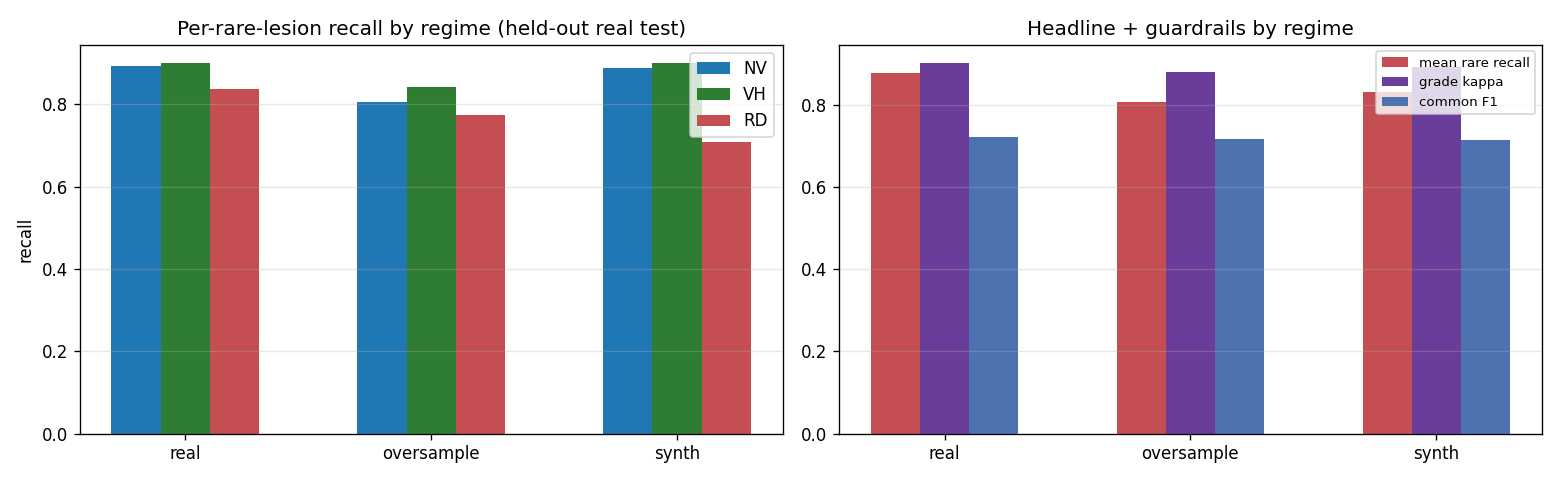
\includegraphics[width=\columnwidth]{exp10-verdict.png}}
\caption{Experiment~X downstream verdict on the held-out real test set. Left:
per-rare-lesion recall by training regime; adding synthetic data does not exceed the
real-only baseline, and RD recall drops. Right: the headline (mean rare recall) and
the two guardrails (grade $\kappa$, common-lesion F1) by regime; the real-only bars
are highest or tied throughout.}
\label{fig:exp10_verdict}
\end{figure}

\subsection{Analysis}
The result is internally consistent: the FID gate predicts it. Synthetic images
$200$--$250$ FID units from the real manifold cannot teach a classifier what a lesion
looks like, so at best they add noise and at worst they mislead---exactly what the RD
column shows. Two secondary observations refine the picture. First, the real-only
baseline is unusually strong on rare recall ($0.878$) because the asymmetric-focal
$+$ contrastive objective is already tuned for the rare classes, so there is little
headroom for augmentation to add. Second, oversampling improves rare \emph{ranking}
(PR-AUC $0.797$ vs.\ $0.653$) while lowering thresholded recall, i.e.\ it trades
sensitivity for precision---useful to note, but the clinically headline number,
recall, still favours the plain real baseline.

\subsection{Discussion}
This is a clean negative result, and a useful one: at a proof-of-concept $64\times64$
resolution, generative augmentation beats neither the real-only baseline nor simple
oversampling for rare-lesion detection. Because the whole pipeline is now built and
measured on a $100\%$-real test set, the finding is trustworthy rather than
anecdotal, and it localises the bottleneck precisely---generation \emph{fidelity},
quantified by the FID gate, not the augmentation methodology. The clear next step is
the higher-resolution latent-diffusion generator the design earmarks; only once its
synthetic-vs-real FID approaches the real-vs-real floor would a downstream benefit be
plausible.

\subsection{Limitations}
The downstream study is single-seed (\texttt{QUICK\_PASS}), so no significance test
accompanies it; the full protocol ($\geq3$ seeds, synthetic amounts
$\{0.5,1,2\}\times$, Wilcoxon) is implemented and gated for a later run. Synthetic
images are $4\times$ upsampled from $64$ to $256$, a resolution-domain confound
quantified by the $64$-vs-$256$ FID gap. Each synthetic image inherits the full
grade$+$lesion label of a random real rare-positive, which is weak supervision on the
grade and common-lesion channels---one reason the guardrails are watched. The
generator itself is the $64$px pixel-space proof-of-concept, not the documented
production LoRA latent-diffusion model.

\subsection{Conclusion}
With the generative-augmentation pipeline fully implemented and evaluated on a
$100\%$-real held-out test set, synthetic rare-lesion images from the $64$px DDPM do
\emph{not} improve rare-class recall over a real-only baseline ($0.833$ vs.\ $0.878$)
or over classic oversampling, and the very high synthetic-vs-real FID ($\approx247$
at $256$px) identifies generation fidelity as the reason. The negative verdict is
itself the contribution: it establishes the evaluation and shows that a
higher-resolution generator, not a different augmentation recipe, is what a future
gain would require.

% ===========================================================================
\section{Experiment XI: Cross-Dataset Zero-Shot and Few-Shot Generalization}
\label{sec:exp11}

\subsection{Objective}
Every preceding experiment trains and evaluates on MMRDR. Experiment~XI asks the
question that decides whether any of it generalises: taken off the shelf, how well
do the trained models grade diabetic retinopathy on \emph{unseen} datasets from
different cameras and populations---first with no adaptation at all (\emph{zero-shot}),
then given only a handful of labelled examples per class (\emph{few-shot})? This is a
grade-only study, because the five-class ICDR severity scale~($0$--$4$) is the one
label space shared across public DR datasets; the seven-lesion vocabulary is
MMRDR-specific and does not transfer.

\subsection{Motivation}
In-domain accuracy can reward dataset-specific shortcuts (a camera's colour cast, a
site's grading habits) that collapse on new data. A cross-dataset test separates a
model that learned transferable retinal pathology from one that memorised a
distribution. Foundation models such as RETFound~\cite{retfound} are pretrained
precisely to transfer, so a like-for-like comparison against a task-specific CNN, on
data neither has seen, is the fair way to judge that claim.

\subsection{Methodology}
Three trained models are frozen and applied to two external datasets. \emph{Zero-shot}
uses each model's own grade head directly, taking $\arg\max$ over its five logits on
the external test split---no fitting whatsoever. \emph{Few-shot} freezes the backbone,
extracts the penultimate feature once, and fits a fresh multinomial logistic head
(standardised features) on $k$ labelled images per class sampled from an external
\emph{support} pool, then predicts the held-out test split. This linear-probe design
is the standard low-variance transfer probe: it isolates feature quality from the
original head's calibration. Each $(k)$ setting is repeated over five independent
support draws; we report the mean and standard deviation, with the zero-shot score as
the $k{=}0$ anchor on the same curve.

\subsection{Experimental Setup}
Implemented in PyTorch on a dual-T4 Kaggle instance. Checkpoints are attached as
read-only inputs and loaded with prefix-stripped state dicts (all three loaded with
zero missing or unexpected tensors). Features are extracted in a single inference
pass per split; the logistic probe is fitted on CPU via scikit-learn. The clean APTOS
labels are auto-preferred when present; the harness detects and reports its inputs so
the run is reproducible.

\subsection{Datasets}
Two genuinely unseen colour-fundus datasets, both on the same $0$--$4$ ICDR scale:
\textbf{APTOS~2019}~\cite{aptos} (the Kaggle Blindness-Detection competition data;
$3{,}662$ labelled images, Indian population) as the clean primary, split
$50/50$ stratified into support/test ($1{,}831$ each); and \textbf{IDRiD}~\cite{idrid}
Disease-Grading, using its official train ($1{,}239$) / test ($309$) partition (an
augmented mirror; see Limitations). Neither appears in any MMRDR training set, and
both differ from MMRDR in camera and cohort, so this is a real domain shift.

\subsection{Preprocessing}
Each external image is preprocessed to match the corresponding model's own training
transform: resize to the model's native size ($512$ for the CFP models, $256$ for the
UWF control), ImageNet normalisation, and---for the multi-scale CNN only---the same
circular fundus mask used in Experiment~I. The UWF control receives standard CFP
preprocessing (no ultra-widefield elliptical mask, whose geometry assumes a UWF field
of view).

\subsection{Models Under Test}
Two CFP models and one deliberate negative control: the \textbf{multi-scale
dual-branch CNN} (MS-LAN, Experiment~I; grade head $\arg\max$; $512$px); the
\textbf{RETFound ViT-L/16} fine-tune (Experiment~II; $512$px; $1024$-d pooled
feature); and the \textbf{UWF supervised-contrastive network} (Experiment~VI) as a
\emph{control} trained on the wrong modality (ultra-widefield), expected to transfer
worst to standard fundus photographs.

\subsection{Evaluation Metrics}
The headline is the quadratic-weighted Cohen's $\kappa$ (QWK), the standard ordinal
DR-grading metric, which is robust to the large shift in grade prior between datasets.
Accuracy, balanced accuracy (mean per-class recall), and macro-F1 are reported
alongside; a $5{\times}5$ confusion matrix is saved per model per dataset.

\subsection{Results}
\emph{Zero-shot} (Table~\ref{tab:exp11_zeroshot}, Fig.~\ref{fig:exp11_zeroshot}). On
the clean APTOS benchmark both CFP models transfer strongly and near-identically---%
RETFound QWK $\mathbf{0.860}$, MS-LAN $0.854$---with the UWF control clearly behind at
$0.689$. On the smaller IDRiD set all three compress into $0.59$--$0.63$ (MS-LAN
$\mathbf{0.626}$), reflecting a harder shift and a $309$-image test set. Throughout,
QWK far exceeds raw accuracy (e.g.\ $0.86$ vs.\ $0.71$ on APTOS): the models get the
ordinal severity right even when the exact class is off, so their errors sit near the
confusion diagonal.

\emph{Few-shot} (Table~\ref{tab:exp11_fewshot}, Fig.~\ref{fig:exp11_fewshot}). A tiny
labelled probe recovers the domain gap where the source head is most mismatched.
RETFound gains most on IDRiD ($0.593\!\to\!0.711$ at $k{=}20$, $+0.118$), and the
wrong-modality UWF control climbs steeply on APTOS ($0.425$ at $k{=}1$ to $0.759$ at
$k{=}20$)---its frozen features are usable even though its own head is not. On clean
APTOS, however, the CFP models' \emph{own} fine-tuned heads already beat a $k$-shot
linear probe (MS-LAN $0.854\!\to\!0.776$; RETFound essentially flat), a legitimate
sign that little headroom remains when the source head is already well matched.

\begin{table}[!t]
\caption{Experiment~XI --- Zero-Shot Grade Transfer to Unseen Datasets}
\label{tab:exp11_zeroshot}
\centering
\setlength{\tabcolsep}{4pt}
\begin{tabular}{|l|l|c|c|c|c|}
\hline
\textbf{Data} & \textbf{Model} & \textbf{QWK} & \textbf{Acc} & \textbf{Bal.\ acc} & \textbf{Mac-F1} \\
\hline
APTOS & MS-LAN (CFP) & $0.854$ & $0.705$ & $0.528$ & $0.505$ \\
APTOS & RETFound (CFP) & $\mathbf{0.860}$ & $\mathbf{0.711}$ & $0.528$ & $0.495$ \\
APTOS & UWF SupCon (ctrl) & $0.689$ & $0.578$ & $0.482$ & $0.412$ \\
\hline
IDRiD & MS-LAN (CFP) & $\mathbf{0.626}$ & $\mathbf{0.511}$ & $0.481$ & $0.478$ \\
IDRiD & RETFound (CFP) & $0.593$ & $0.476$ & $0.398$ & $0.404$ \\
IDRiD & UWF SupCon (ctrl) & $0.598$ & $0.375$ & $0.431$ & $0.364$ \\
\hline
\multicolumn{6}{|l|}{\footnotesize Best per dataset in \textbf{bold}. Grade QWK $=$
quadratic-weighted $\kappa$;} \\
\multicolumn{6}{|l|}{\footnotesize Bal.\ acc $=$ mean per-class recall. APTOS test
$n{=}1{,}831$, IDRiD $n{=}309$.} \\
\hline
\end{tabular}
\end{table}

\begin{table}[!t]
\caption{Experiment~XI --- Few-Shot Grade QWK vs.\ Shots per Class (mean$_{\pm\text{std}}$, 5 episodes)}
\label{tab:exp11_fewshot}
\centering
\setlength{\tabcolsep}{3pt}
\begin{tabular}{|l|c|c|c|c|c|}
\hline
\textbf{Model} & \textbf{$k{=}0$} & \textbf{$k{=}1$} & \textbf{$k{=}5$} & \textbf{$k{=}10$} & \textbf{$k{=}20$} \\
\hline
\multicolumn{6}{|l|}{\emph{APTOS 2019 (clean)}} \\
\hline
MS-LAN & $0.854$ & $.691_{\pm.03}$ & $.749_{\pm.04}$ & $.770_{\pm.01}$ & $.776_{\pm.03}$ \\
RETFound & $0.860$ & $.813_{\pm.05}$ & $.844_{\pm.01}$ & $\mathbf{.851}_{\pm.00}$ & $.850_{\pm.01}$ \\
UWF (ctrl) & $0.689$ & $.425_{\pm.15}$ & $.575_{\pm.13}$ & $.712_{\pm.02}$ & $.759_{\pm.03}$ \\
\hline
\multicolumn{6}{|l|}{\emph{IDRiD (augmented mirror)}} \\
\hline
MS-LAN & $0.626$ & $.540_{\pm.09}$ & $.591_{\pm.06}$ & $.627_{\pm.04}$ & $.676_{\pm.04}$ \\
RETFound & $0.593$ & $.589_{\pm.07}$ & $.660_{\pm.05}$ & $.697_{\pm.03}$ & $\mathbf{.711}_{\pm.03}$ \\
UWF (ctrl) & $0.598$ & $.254_{\pm.12}$ & $.480_{\pm.04}$ & $.552_{\pm.03}$ & $.575_{\pm.02}$ \\
\hline
\multicolumn{6}{|l|}{\footnotesize $k{=}0$ is the zero-shot anchor (each model's own
head). $k{>}0$ is a frozen-} \\
\multicolumn{6}{|l|}{\footnotesize backbone logistic probe on $k$ images/class.
IDRiD few-shot is optimistic (augmentation).} \\
\hline
\end{tabular}
\end{table}

\begin{figure}[!t]
\centerline{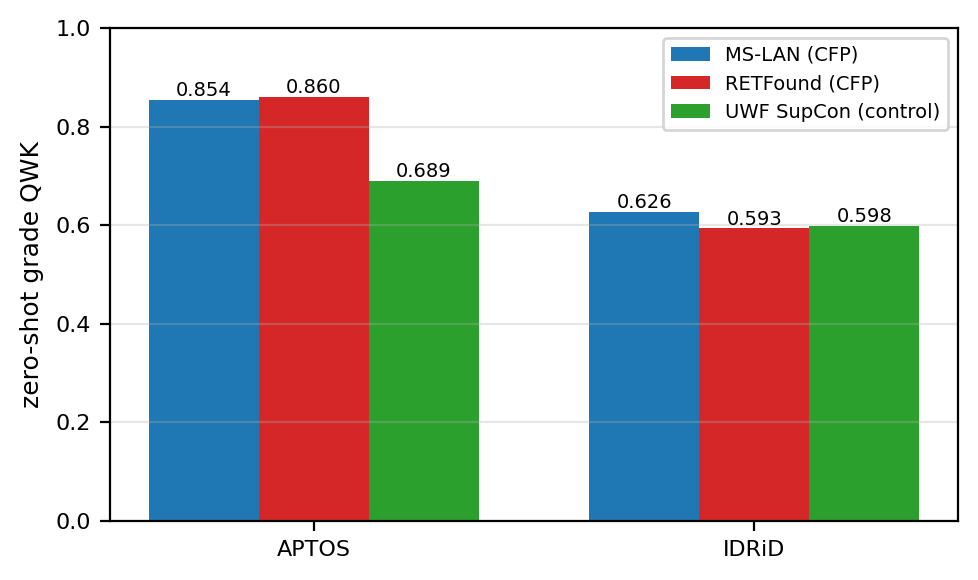
\includegraphics[width=\columnwidth]{exp11-zeroshot.png}}
\caption{Experiment~XI zero-shot grade QWK on two unseen external datasets. On the
clean APTOS benchmark the two CFP models transfer strongly and near-identically
(RETFound $0.860$, MS-LAN $0.854$) while the ultra-widefield control lags at $0.689$;
on the harder, smaller IDRiD set the three compress to $0.59$--$0.63$.}
\label{fig:exp11_zeroshot}
\end{figure}

\begin{figure}[!t]
\centerline{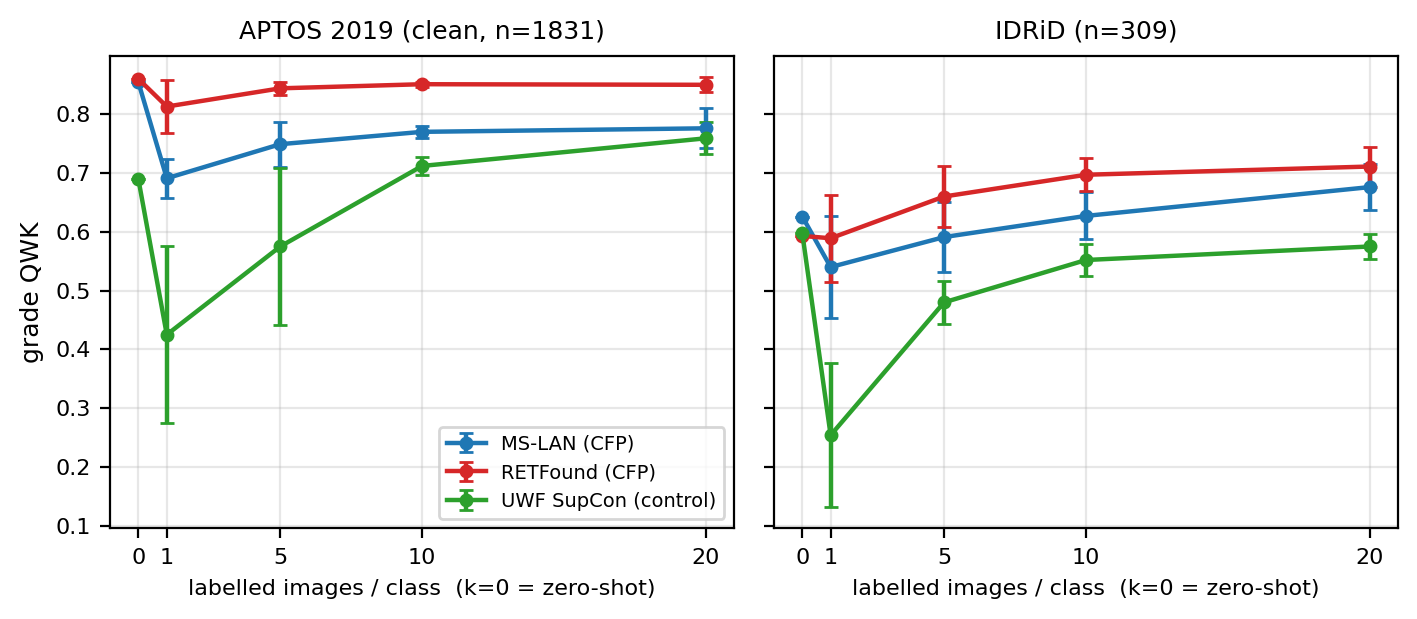
\includegraphics[width=\columnwidth]{exp11-fewshot.png}}
\caption{Experiment~XI few-shot transfer: grade QWK versus labelled images per class,
with the zero-shot score as the $k{=}0$ anchor (mean$\pm$std over five support draws).
A small probe recovers the domain gap most where the source head is mismatched
(RETFound on IDRiD; the wrong-modality UWF control on APTOS), whereas on clean APTOS
the CFP models' own heads already match or exceed the probe.}
\label{fig:exp11_fewshot}
\end{figure}

\subsection{Analysis}
Three patterns are consistent across both datasets. First, \emph{the foundation model
is the best all-round generaliser}: RETFound is top zero-shot on the clean benchmark
and shows the largest few-shot recovery on the shifted one, exactly the behaviour its
pretraining promises. Second, \emph{modality matters}: the UWF control transfers
measurably worse than the CFP models on the clean benchmark ($0.689$ vs.\ $\sim0.86$
QWK, and the lowest balanced accuracy everywhere). It does not collapse to chance---%
grade QWK is ordinal-tolerant, and a wrong-modality retinal network still ranks
severity partially---but the gap confirms the CFP models' transfer is modality-matched
rather than a metric artefact. Third, \emph{few-shot value is inversely related to
source-head fit}: the probe helps precisely when the original head is domain-shifted
and adds nothing when it is already well calibrated.

\subsection{Discussion}
The concluding message of the report is positive: the CFP models trained on MMRDR do
not merely fit their own distribution---they grade an unseen dataset zero-shot at a
quadratic $\kappa$ of $0.86$, and a foundation-model backbone transfers best, matching
the premise on which the RETFound baseline (Experiment~II) was chosen. The persistent
gap between QWK and balanced accuracy is the same rare-class weakness this report has
tracked throughout: minority grades ($1$, $3$, $4$) remain under-recalled off-domain,
so the strong $\kappa$ reflects correct ordering more than per-class sensitivity. The
few-shot curves suggest the cheapest route to a deployable cross-site grader is not
retraining but a small labelled calibration set fitted on frozen foundation-model
features.

\subsection{Limitations}
IDRiD here is an augmented mirror ($1{,}239/309$ rather than the standard $413/103$),
so near-duplicate images can straddle its support and test splits and its
\emph{few-shot} numbers should be read as optimistic; the zero-shot numbers, which
never fit on the support pool, are unaffected. Only one fully clean external set
(APTOS) is used, and zero-shot scores are single point estimates without bootstrap
confidence intervals. The study is grade-only: lesion transfer is out of scope because
external datasets do not share the seven-lesion scheme. Few-shot uses a linear probe,
not full fine-tuning, and the transfer is CFP-only---no public ultra-widefield or OCT
grading set exists to test the UWF/OCT models in kind, which is why the UWF model
appears only as a control.

\subsection{Conclusion}
Evaluated on data they had never seen, the MMRDR-trained CFP models generalise: both
grade APTOS zero-shot at QWK $\approx0.85$--$0.86$, the RETFound foundation model
transfers best on the clean benchmark and recovers most from a handful of labelled
examples on the shifted one, and a wrong-modality control transfers measurably worse.
The experiment closes the report by showing that the representations it built are not
dataset-bound, and that a foundation-model backbone plus a light few-shot calibration
is the most promising path to cross-site DR grading.

% ===========================================================================
\section{Conclusion}
\label{sec:conclusion}
This report documented ten multi-task deep-learning experiments on the MMRDR
dataset, each jointly performing DR severity grading and seven-way lesion
detection, and a concluding cross-dataset generalization study (Experiment~XI),
eleven in total. The first three establish modality baselines. On color fundus
photography, the multi-scale dual-branch convolutional network (Experiment~I)
reached $82.91\%$ validation grade accuracy, while the fine-tuned RETFound
foundation model (Experiment~II) reached $80.94\%$ on the dataset's official
held-out test split, reproducing three of the four published baseline metrics
within their $95\%$ confidence intervals. These two numbers are close in magnitude
but are \emph{not} directly comparable: Experiment~II is the only experiment
evaluated on a genuine held-out test partition, whereas Experiment~I reports
validation accuracy on a random split. Experiment~II also illustrates a
methodological point that generalises beyond this dataset---an earlier attempt
reported $66.50\%$, which an audit traced not to the method but to a silent
weight-loading failure in which only $4$ of $294$ tensors transferred, and to a
layer-freezing routine that never executed. On the more challenging ultra-widefield
modality, the feature-pyramid network with spatial attention (Experiment~III)
reached $74.48\%$.

The remaining five experiments form a focused thread on the ultra-widefield
modality: making the model sensitive to the rare, sight-threatening lesions of
proliferative DR (NV, VH, RD), attacking the problem from four angles---loss
weighting, loss shape, representation, and data sampling. Experiment~IV re-weights
the lesion loss by combined statistical rarity and clinical risk, lifting recall on
the highest-risk lesions (RD $0.79$, VH $0.77$, NV $0.68$) at the intended cost of
common-lesion recall. Experiment~V replaces the objective with an asymmetric,
false-negative-penalised focal loss, reaching a quadratic $\kappa$ of $0.92$ and
lesion AUC of $0.95$. Experiment~VI shapes the feature space with a two-depth
supervised contrastive auxiliary. Experiment~VII learns the multi-task weights via
homoscedastic uncertainty and reaches the study's best rare-lesion detection
(lesion F1 up to $0.778$, AUROC up to $0.961$; rare recall NV/VH/RD
$=0.89/0.95/0.96$), though its lesion weight saturated at the numerical clamp.
Experiment~VIII holds the network fixed and adapts the training \emph{sampler} with
a recall-driven curriculum, pushing RD recall to $1.0$ and reaching $\kappa=0.923$
on a stratified split. Two further experiments probe the architecture and the data
supply. Experiment~IX is a controlled, capacity-matched ablation on a held-out test
split that finds a dedicated rare-lesion head does not beat---and slightly harms---a
shared head ($0.816$ vs.\ $0.890$ mean rare recall), indicating head topology is not
the bottleneck. Experiment~X completes the generative-augmentation study: a $64$px
conditional-diffusion generator's synthetic rare-lesion images do \emph{not} improve
downstream rare-class recall over a real-only baseline ($0.833$ vs.\ $0.878$) or over
oversampling, and a very high synthetic-vs-real FID ($\approx247$) localises the
bottleneck to generation fidelity---a clean negative result that motivates a
higher-resolution generator. Finally, Experiment~XI steps outside MMRDR entirely and
tests cross-dataset generalization: applied to unseen external fundus datasets
(APTOS~2019 and IDRiD), the two CFP models grade APTOS zero-shot at a quadratic
$\kappa$ of $\approx0.85$--$0.86$, the RETFound foundation model transfers best and
recovers most from a few labelled examples, and a wrong-modality UWF control transfers
measurably worse---evidence that the learned representations are not dataset-bound.
Across the ten trained experiments, focal-family objectives
stabilised training under class imbalance, and Grad-CAM confirmed that predictions
were driven by clinically plausible retinal regions. Tables~\ref{tab:overall}
and~\ref{tab:uwf_rare} summarise the comparison. Future work includes multi-seed,
same-split comparisons with significance testing, a wider uncertainty clamp,
higher-resolution foundation-model fine-tuning, calibrating the risk weights to a
clinical utility function, running the generative-augmentation study, and unified
multimodal training.

\begin{table}[!t]
\caption{Summary of the Ten Experiments}
\label{tab:overall}
\centering
\setlength{\tabcolsep}{3pt}
\begin{tabular}{|l|l|c|}
\hline
\textbf{Exp.} & \textbf{Model / lever (modality)} & \textbf{Grade acc.} \\
\hline
I & Multi-scale dual-branch CNN (CFP) & $0.8291$ \\
II & RETFound ViT-L/16 fine-tune (CFP) & $0.8094$\,\textsuperscript{$\ast$} \\
III & FPN + spatial attention (UWF) & $0.7448$ \\
IV & Clinically-weighted lesion loss (UWF) & $0.7650$ \\
V & Asymmetric FN-penalised loss (UWF) & $0.7578$\,\textsuperscript{a} \\
VI & Supervised contrastive auxiliary (UWF) & $0.7645$\,\textsuperscript{b} \\
VII & Learned uncertainty weighting (UWF) & $0.7554$\,\textsuperscript{c} \\
VIII & Recall-driven resampling (UWF) & ---\,\textsuperscript{d} \\
IX & Shared vs.\ separate heads (UWF) & ---\,\textsuperscript{e} \\
X & Synthetic generation (UWF) & ---\,\textsuperscript{f} \\
\hline
\multicolumn{3}{|l|}{\footnotesize \textsuperscript{$\ast$}Official held-out test
split (not validation); paper $0.822$.} \\
\multicolumn{3}{|l|}{\footnotesize \textsuperscript{a}Selected ckpt, ep~$16$; peak
$0.7770$. \textsuperscript{b}Plateau peak, ep~$28$--$37$.} \\
\multicolumn{3}{|l|}{\footnotesize \textsuperscript{c}Selected ckpt, ep~$21$; peak
$0.7645$. \textsuperscript{d}$\kappa=0.923$ (acc.\ not logged).} \\
\multicolumn{3}{|l|}{\footnotesize \textsuperscript{e}Test split; best macro-F1
$0.707$, $\kappa=0.914$. \textsuperscript{f}Verdict: synthetic does} \\
\multicolumn{3}{|l|}{\footnotesize not beat real-only rare recall ($0.833$ vs.\ $0.878$).} \\
\hline
\end{tabular}
\end{table}

\begin{table}[!t]
\caption{UWF Rare-Lesion Experiments --- Validation Metrics}
\label{tab:uwf_rare}
\centering
\setlength{\tabcolsep}{3pt}
\begin{tabular}{|l|c|c|c|c|}
\hline
\textbf{Exp. (lever)} & \textbf{Grade $\kappa$} & \textbf{Lesion F1} &
\textbf{Lesion AUC} & \textbf{RD rec.} \\
\hline
IV (clinical wts) & --- & $0.56$ & --- & $0.79$ \\
V (asym.\ loss) & $0.9208$ & $0.7151$ & $0.9504$ & --- \\
VI (contrastive) & $0.9223$ & $0.7390$ & $0.9523$ & --- \\
VII (uncertainty) & $0.9211$ & $0.7779$ & $0.9605$ & $0.958$ \\
VIII (resampling)\textsuperscript{$\dagger$} & $0.9234$ & $0.7088$ & $0.9455$ & $1.00$ \\
\hline
\multicolumn{5}{|l|}{\footnotesize Best validation value per column. Lesion F1/AUC
macro-averaged;} \\
\multicolumn{5}{|l|}{\footnotesize ``---'' = not computed. RD rec.\ = retinal-detach.\
recall. \textsuperscript{$\dagger$}Stratified} \\
\multicolumn{5}{|l|}{\footnotesize split---not directly comparable to the other rows.} \\
\hline
\end{tabular}
\end{table}

% ===========================================================================
\begin{thebibliography}{00}
\bibitem{mmrdr}
Z.~Tang, L.~Wang, Z.~Guo, Q.~Liang, S.~Xue, C.~Feng, L.~Ran, L.~Chen,
X.~Wang, and J.~Li, ``A multimodal retinal image dataset for diabetic
retinopathy detection using foundation models,'' \emph{Scientific Data}, 2026,
in press, doi:\ 10.1038/s41597-026-07005-9.

\bibitem{resnet}
K.~He, X.~Zhang, S.~Ren, and J.~Sun, ``Deep residual learning for image
recognition,'' in \emph{Proc. IEEE Conf. Comput. Vis. Pattern Recognit.
(CVPR)}, 2016, pp.\ 770--778.

\bibitem{focalloss}
T.-Y.~Lin, P.~Goyal, R.~Girshick, K.~He, and P.~Doll\'ar, ``Focal loss for
dense object detection,'' in \emph{Proc. IEEE Int. Conf. Comput. Vis. (ICCV)},
2017, pp.\ 2980--2988.

\bibitem{gradcam}
R.~R.~Selvaraju, M.~Cogswell, A.~Das, R.~Vedantam, D.~Parikh, and D.~Batra,
``Grad-CAM: Visual explanations from deep networks via gradient-based
localization,'' in \emph{Proc. IEEE Int. Conf. Comput. Vis. (ICCV)}, 2017,
pp.\ 618--626.

\bibitem{retfound}
Y.~Zhou \emph{et al.}, ``A foundation model for generalizable disease detection
from retinal images,'' \emph{Nature}, vol.~622, pp.\ 156--163, 2023.

\bibitem{fpn}
T.-Y.~Lin, P.~Doll\'ar, R.~Girshick, K.~He, B.~Hariharan, and S.~Belongie,
``Feature pyramid networks for object detection,'' in \emph{Proc. IEEE Conf.
Comput. Vis. Pattern Recognit. (CVPR)}, 2017, pp.\ 2117--2125.

\bibitem{cbam}
S.~Woo, J.~Park, J.-Y.~Lee, and I.~S.~Kweon, ``CBAM: Convolutional block
attention module,'' in \emph{Proc. Eur. Conf. Comput. Vis. (ECCV)}, 2018,
pp.\ 3--19.

\bibitem{supcon}
P.~Khosla, P.~Teterwak, C.~Wang, A.~Sarna, Y.~Tian, P.~Isola, A.~Maschinot,
C.~Liu, and D.~Krishnan, ``Supervised contrastive learning,'' in \emph{Adv.
Neural Inf. Process. Syst. (NeurIPS)}, vol.~33, 2020, pp.\ 18661--18673.

\bibitem{asl}
E.~Ben-Baruch, T.~Ridnik, N.~Zamir, A.~Noy, I.~Friedman, M.~Protter, and
L.~Zelnik-Manor, ``Asymmetric loss for multi-label classification,'' in
\emph{Proc. IEEE/CVF Int. Conf. Comput. Vis. (ICCV)}, 2021, pp.\ 82--91.

\bibitem{uncertainty}
A.~Kendall, Y.~Gal, and R.~Cipolla, ``Multi-task learning using uncertainty to
weigh losses for scene geometry and semantics,'' in \emph{Proc. IEEE Conf.
Comput. Vis. Pattern Recognit. (CVPR)}, 2018, pp.\ 7482--7491.

\bibitem{effnum}
Y.~Cui, M.~Jia, T.-Y.~Lin, Y.~Song, and S.~Belongie, ``Class-balanced loss based
on effective number of samples,'' in \emph{Proc. IEEE/CVF Conf. Comput. Vis.
Pattern Recognit. (CVPR)}, 2019, pp.\ 9268--9277.

\bibitem{ddpm}
J.~Ho, A.~Jain, and P.~Abbeel, ``Denoising diffusion probabilistic models,'' in
\emph{Adv. Neural Inf. Process. Syst. (NeurIPS)}, vol.~33, 2020,
pp.\ 6840--6851.

\bibitem{cfg}
J.~Ho and T.~Salimans, ``Classifier-free diffusion guidance,'' in \emph{NeurIPS
Workshop on Deep Generative Models and Downstream Applications}, 2021.

\bibitem{ldm}
R.~Rombach, A.~Blattmann, D.~Lorenz, P.~Esser, and B.~Ommer, ``High-resolution
image synthesis with latent diffusion models,'' in \emph{Proc. IEEE/CVF Conf.
Comput. Vis. Pattern Recognit. (CVPR)}, 2022, pp.\ 10684--10695.

\bibitem{fid}
M.~Heusel, H.~Ramsauer, T.~Unterthiner, B.~Nessler, and S.~Hochreiter, ``GANs
trained by a two time-scale update rule converge to a local Nash equilibrium,''
in \emph{Adv. Neural Inf. Process. Syst. (NeurIPS)}, vol.~30, 2017,
pp.\ 6626--6637.

\bibitem{aptos}
Asia Pacific Tele-Ophthalmology Society (APTOS), ``APTOS 2019 Blindness Detection,''
Kaggle Competition, 2019. [Online]. Available:
\url{https://www.kaggle.com/c/aptos2019-blindness-detection}

\bibitem{idrid}
P.~Porwal, S.~Pachade, R.~Kamble, M.~Kokare, G.~Deshmukh, V.~Sahasrabuddhe, and
F.~M\'eriaudeau, ``Indian Diabetic Retinopathy Image Dataset (IDRiD): A database for
diabetic retinopathy screening research,'' \emph{Data}, vol.~3, no.~3, p.~25, 2018.
\end{thebibliography}

\end{document}
